\documentclass[10pt]{article}
\usepackage[vietnamese]{babel}
\usepackage[utf8]{inputenc}
\usepackage[T5]{fontenc}
\usepackage{graphicx}
\usepackage[export]{adjustbox}
\graphicspath{ {./images/} }
\usepackage{amsmath}
\usepackage{amsfonts}
\usepackage{amssymb}
\usepackage[version=4]{mhchem}
\usepackage{stmaryrd}
\usepackage{caption}
\usepackage{multirow}
\usepackage{hyperref}
\hypersetup{colorlinks=true, linkcolor=blue, filecolor=magenta, urlcolor=cyan,}
\urlstyle{same}

%New command to display footnote whose markers will always be hidden
\let\svthefootnote\thefootnote
\newcommand\blfootnotetext[1]{%
  \let\thefootnote\relax\footnote{#1}%
  \addtocounter{footnote}{-1}%
  \let\thefootnote\svthefootnote%
}

%Overriding the \footnotetext command to hide the marker if its value is `0`
\let\svfootnotetext\footnotetext
\renewcommand\footnotetext[2][?]{%
  \if\relax#1\relax%
    \ifnum\value{footnote}=0\blfootnotetext{#2}\else\svfootnotetext{#2}\fi%
  \else%
    \if?#1\ifnum\value{footnote}=0\blfootnotetext{#2}\else\svfootnotetext{#2}\fi%
    \else\svfootnotetext[#1]{#2}\fi%
  \fi
}

\def\AA{\mathring{\mathrm{A}}}

\begin{document}
\captionsetup{singlelinecheck=false}
\section*{Chuong 1. ESTERR - LIPID. XA PHONG VA CHÍT GHAT RÚA}
\begin{center}
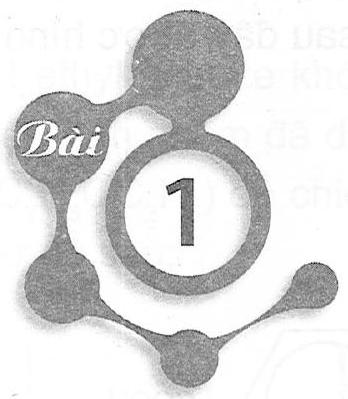
\includegraphics[max width=\textwidth]{2025_10_23_de6f5713836e4e91b3c8g-001}
\end{center}

\section*{ESTER - LIPID}
1.1. Có bao nhiêu ester có công thức phân tử $\mathrm{C}_{4} \mathrm{H}_{8} \mathrm{O}_{2}$ ?\\
A. 2 .\\
B. 3 .\\
C. 4 .\\
D. 5 .\\
1.2. Có bao nhiêu hợp chất hữu cơ đơn chức khác nhau có công thức phân tử $\mathrm{C}_{3} \mathrm{H}_{6} \mathrm{O}_{2}$ ?\\
A. 2 .\\
B. 3 .\\
C. 4 .\\
D. 5 .\\
1.3. Có 4 ester no, đơn chức, mạch hở được kí hiệu ngẫu nhiên lần lượt là $X, Y, Z, T$. Phân tử ester của mỗi chất nêu trên đều tạo bởi các carboxylic acid mạch không phân nhánh và ethyl alcohol. Độ tan của 4 ester được cho ở bảng sau:

\begin{center}
\begin{tabular}{|c|c|c|c|c|}
\hline
Ester & X & Y & Z & T \\
\hline
Độ tan ( $\mathrm{g} / 100 \mathrm{~g}$ nước) & 8,7 & 10,5 & 2,2 & 4,9 \\
\hline
\end{tabular}
\end{center}

Trong số 4 ester trên, ester có nhiều nguyên tử carbon nhất trong phân tử là\\
A. Y.\\
B. T.\\
C. X.\\
D. Z.\\
1.4. Cho 4 chất sau: butan-1-ol (1), butanoic acid (2), ethyl acetate (3) và pentan-2-ol (4). Chất có nhiệt độ sôi thấp nhất trong 4 chất nêu trên là\\
A. (1).\\
B. (2).\\
C. (3).\\
D. (4).\\
1.5. Tính chất nào sau đây không phải là tính chất thích hợp giúp ethyl methanoate $\left(\mathrm{HCOOC}_{2} \mathrm{H}_{5}\right)$ được sử dụng trong sản xuất một số loại nước hoa?\\
A. Khả năng dễ cháy.\\
B. Có mùi thơm dễ chịu\\
C. Không độc hại.\\
D. Nhiệt độ sôi thấp.\\
1.6. Ngoài sản phẩm phụ là nước, chất hữu cơ nào sau đây được hình thành từ phản ứng hoá học đã cho?\\
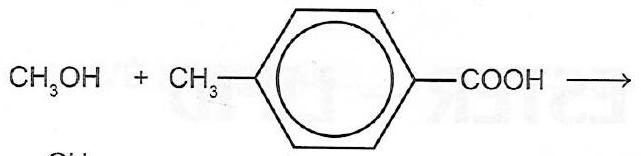
\includegraphics[max width=\textwidth, center]{2025_10_23_de6f5713836e4e91b3c8g-002}

A.\\
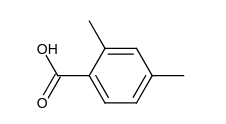
\includegraphics{smile-a3243636d539d96d8d9955ae4d507a897c702a21}

B.\\
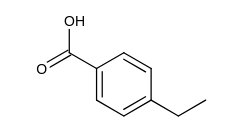
\includegraphics{smile-3fea05a2e410e6df96031cb05f3a10adf5b3790c}

C.\\
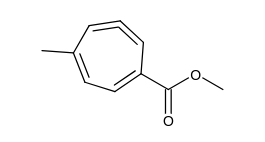
\includegraphics{smile-069c43fd1d84552383f4670fe7f7e3bacd6b8ae1}

D.\\
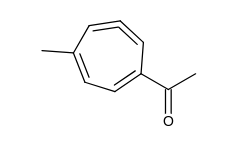
\includegraphics{smile-6cae12455a4cc6a2def442f07a3d18c73b9ae39d}\\
1.7. Aspirin là một trong những loại thuốc giảm đau, hạ sốt được sử dụng rộng rãi trên toàn thế giới. Aspirin có công thức cấu tạo như sau:\\
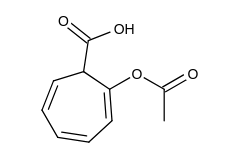
\includegraphics{smile-d4a2c4ee4a4bcf2ae9fa5567446cb7850b8b720e}

Trong điều kiện ẩm ướt, aspirin có thể bị thuỷ phân để tạo thành salicylic acid và acetic acid. Công thức cấu tạo nào sau đây là của salicylic acid?

A.\\
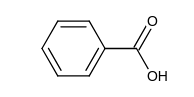
\includegraphics{smile-2ae7efd825bcf4e7cab6714b5e0d54942c742e9e}

B.\\
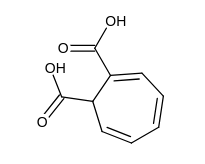
\includegraphics{smile-0639e18d43051fab89dc474d5a4009662470e114}

C.\\
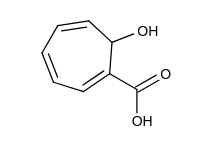
\includegraphics{smile-7657c68c5d8569f70a0806b76fe331c09a9f3f26}

D.\\
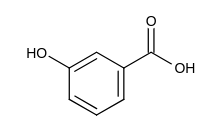
\includegraphics{smile-6abfa1662fb0693a3c2c343b6becface9723bbc8}\\
1.8. Một nhóm học sinh đã thực hiện phản ứng điều chế ethyl acetate từ nguyên liệu ban đầu là acetic acid và ethanol trong phòng thí nghiệm. Khi phản ứng kết thúc, nhóm đã thu được hỗn hợp sản phẩm gồm ethyl acetate và acetic acid, ethanol còn dư theo phương trình hoá học:

$$
\mathrm{CH}_{3} \mathrm{COOH}+\mathrm{C}_{2} \mathrm{H}_{5} \mathrm{OH} \stackrel{\mathrm{H}^{+}, \mathrm{t}^{\circ}}{\rightleftharpoons} \mathrm{CH}_{3} \mathrm{COOC}_{2} \mathrm{H}_{5}+\mathrm{H}_{2} \mathrm{O}
$$

Vì ethyl acetate không phân cực, còn acetic acid và ethanol đều phân cực nên nhóm đã dùng dung môi hữu cơ không phân cực diethyl ether $\left(\mathrm{C}_{2} \mathrm{H}_{5} \mathrm{OC}_{2} \mathrm{H}_{5}\right)$ để chiết ethyl acetate ra khỏi hỗn hợp sau phản ứng theo sơ đồ sau:\\
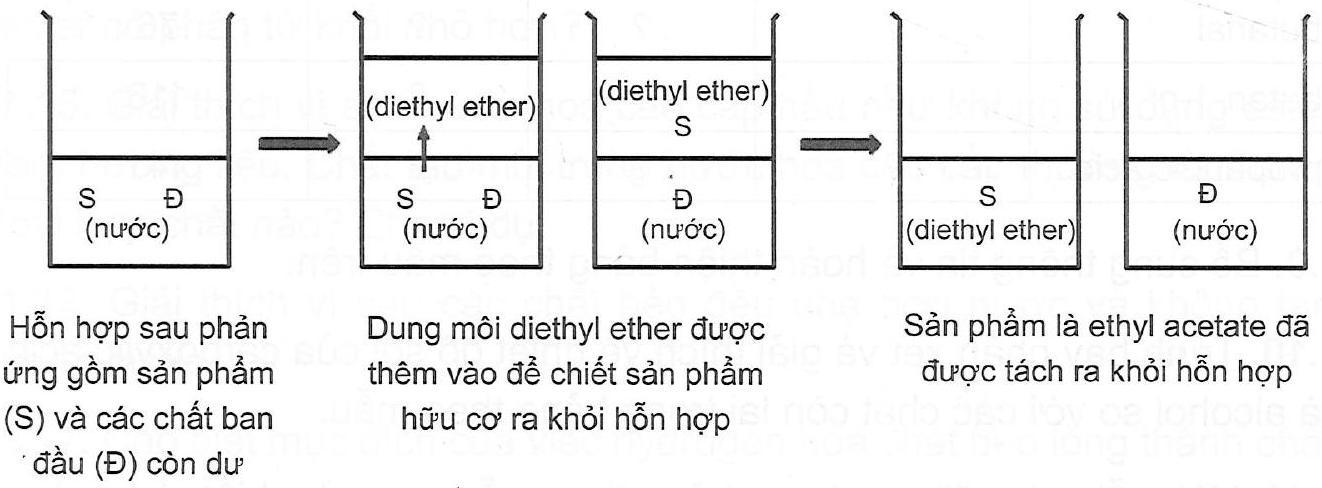
\includegraphics[max width=\textwidth, center]{2025_10_23_de6f5713836e4e91b3c8g-003}

Cho các phát biểu sau về thí nghiệm của nhóm:\\
a) Diethyl ether là dung môi chiết lí tưởng trong thí nghiệm trên vì ethyl acetate tan tốt trong dung môi này, còn acetic acid và ethanol lại tan tốt trong nước.\\
b) Bằng phương pháp chưng cất đơn giản, ta có thể tách ethyl acetate ra khỏi dung môi diethyl ether sau khi chiết.\\
c) Do diethyl ether có nhiệt độ sôi thấp hơn nhiều so với ethyl acetate $\left(34,6^{\circ} \mathrm{C}\right.$ so với $\left.77,1^{\circ} \mathrm{C}\right)$ nên có thể thu được ethyl acetate sau khi chiết bằng cách dùng đèn cồn đun nhẹ cho dung môi diethyl ether bay hơi.\\
d) Để an toàn, ta có thể dùng nước nóng liên tục tưới lên bình cầu trong phương pháp chưng cất đơn giản để tách ethyl acetate ra khỏi dung môi diethyl ether sau khi chiết.

Số phát biểu đúng là\\
A. 1 .\\
B. 2.\\
C. 3 .\\
D. 4 .

Nhiệt độ sôi của một số họp chất hữu cơ được cho ở bảng dưới đây. Quan sát loảng dưới để trả lời các câu 1.9 và 1.10.

\begin{center}
\begin{tabular}{|l|l|l|l|l|}
\hline
Tên gọi & Công thức cấu tạo & Phân loại & Phân tử' khối & Nhiệt độ sôi ( ${ }^{\circ} \mathrm{C}$ ) \\
\hline
diethyl ether & ? & ? & ? & 34 \\
\hline
ethyl formate & ? & ? & ? & 54 \\
\hline
methyl acetate & ? & ? & ? & 57 \\
\hline
butanal & ? & ? & ? & 76 \\
\hline
butan-1-ol & ? & ? & ? & 118 \\
\hline
propanoic acid & ? & ? & ? & 141 \\
\hline
\end{tabular}
\end{center}

1.9. Bổ sung thông tin và hoàn thiện bảng theo mẫu trên.\\
1.10. Trình bày nhận xét và giải thích về nhiệt độ sôi của carboxylic acid và alcohol so với các chất còn lại trong bảng theo mẫu.\\
1.11. Với mỗi ester đã cho trong bảng theo mẫu sau, cho biết chúng tạo bởi từ nhữung carboxylic acid và alcohol nào?

\begin{center}
\begin{tabular}{|l|l|l|}
\hline
Ester & Acid tạo thành và tên gọi & Alcohol tạo thành và tên gọi \\
\hline
$\mathrm{C}_{2} \mathrm{H}_{5} \mathrm{COOCH}_{3}$ & ? & ? \\
\hline
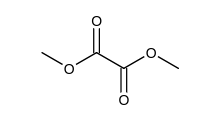
\includegraphics{smile-aeeb027feedf6e2574c4147257b3613f3be763ec} & ? & ? \\
\hline
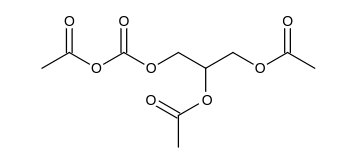
\includegraphics{smile-d0bbfb3a01fd29156ffd06b304320150888a93b9} & ? & ? \\
\hline
\end{tabular}
\end{center}

1.12. Cho 6 hợp chất sau: $\mathrm{HCOOH}, \mathrm{CH}_{3} \mathrm{CH}_{2} \mathrm{CH}_{2} \mathrm{COOH}, \mathrm{CH}_{3} \mathrm{CH}_{2} \mathrm{CH}_{2} \mathrm{CH}_{2} \mathrm{OH}$, $\mathrm{CH}_{3} \mathrm{COOCH}_{2} \mathrm{CH}_{3}, \mathrm{CH}_{3} \mathrm{CH}_{2} \mathrm{CH}_{2} \mathrm{CH}_{2} \mathrm{CH}_{2} \mathrm{OH}$ và $\mathrm{HCOOCH}_{2} \mathrm{CH}_{2} \mathrm{CH}_{2} \mathrm{CH}_{3}$. Hoàn thiện bảng theo mẫu sau. Giải thích.

\begin{center}
\begin{tabular}{|c|c|c|c|}
\hline
Họp chất & \begin{tabular}{c}
Nhiệt độ \\
sôi $\left({ }^{\circ} \mathrm{C}\right)$ \\
\end{tabular} & Hợp chất & \begin{tabular}{c}
Nhiệt độ \\
sôi $\left({ }^{\circ} \mathrm{C}\right)$ \\
\end{tabular} \\
\hline
HCOOH & 100,8 & $?$ & 164 \\
\hline
$?$ & 117,7 & $\mathrm{CH}_{3} \mathrm{CH}_{2} \mathrm{CH}_{2} \mathrm{CH}_{2} \mathrm{CH}_{2} \mathrm{OH}$ & 138 \\
\hline
$\mathrm{HCOOCH}_{2} \mathrm{CH}_{2} \mathrm{CH}_{2} \mathrm{CH}_{3}$ & 107 & $?$ & 77 \\
\hline
\end{tabular}
\end{center}

1.13. Thuỷ phân hoàn toàn triglyceride $X$ thu được glycerol và 3 acid béo là lauric acid, palmitic acid và oleic acid. $X$ có thể có bao nhiêu công thức cấu tạo?\\
1.14. Vì sao ester có phân tử khối lớn có mùi thơm nhẹ hơn so với các ester có phân tử khối nhỏ hơn?\\
1.15. Giải thích vì sao nước hoa cao cấp hầu như không sử dụng ester làm hương liệu. Chất tạo mùi trong nước hoa cao cấp thường là những loại hợp chất nào? Cho ví dụ.\\
1.16. Giải thích vì sao các chất béo đều nhẹ hơn nước và không tan trong nước.\\
1.17. Cho biết mục đích của việc hydrogen hoá chất béo lỏng thành chất béo rắn.\\
1.18. Một nhóm học sinh dưới sự hướng dẫn của giáo viên muốn thực hiện thí nghiệm điều chế ester nên đã tiến hành theo các bước sau.\\
Bước 1: Cho vào bình cầu đáy tròn 22 mL pentyl alcohol ( $\mathrm{D}=0,81 \mathrm{~g} / \mathrm{mL}$ ) và V mL acetic acid ( $\mathrm{D}=1,05 \mathrm{~g} / \mathrm{mL}$ ).\\
Bước 2: Thêm tiếp vào bình cầu đó 4 mL dung dịch sulfuric acid đặc và một ít đá bọt. Đun hồi lưu hỗn hợp trong khoảng 30 phút.

Bước 3: Sau một thời gian, nhóm học sinh tiến hành cân khối lượng ester thu được sau khi tách khỏi hỗn hợp và làm sạch, cân hiển thị khối lượng 17 g .\\
a) Xác định V để tỉ lệ mol giữa pentyl alcohol và acetic acid là $1: 1$.\\
b) Đá bọt là gì? Nêu vai trò của đá bọt trong thí nghiệm trên.\\
c) Cho biết đặc điểm của phản ứng xảy ra trong thí nghiệm đã nêu.\\
d) Tính hiệu suất của phản ứng ester hoá trên.\\
e) Trong hỗn hợp phản ứng ban đầu ở bình cầu đáy tròn, nhóm thí nghiệm còn cho thêm một ít hạt silica gel có màu xanh vào trước khi đun hồi lưu.

\begin{itemize}
  \item Mục đích của việc thêm vào các hạt silica gel là gì?
  \item Giải thích vì sao khi kết thúc thí nghiệm, các hạt silica gel từ màu xanh chuyển sang màu hồng.\\
1.19. Vì sao nói chất béo là thức ăn quan trọng của con người?\\
1.20. Vì sao trong thực tế, dầu thực vật tuy chứa chủ yếu chất béo không no nhưng lại khó bị ôi thiu hơn mỡ động vật chứa chủ yếu chất béo no?\\
1.21. Một trong những cách làm mới lại bề mặt các vật dụng bằng gỗ đó là sử dụng sáp ong để đánh bóng. Sáp ong là một lipid với thành phần chính là myricyl palmitate. Đây là một ester có mạch không phân nhánh, công thức phân tử là $\mathrm{C}_{46} \mathrm{H}_{92} \mathrm{O}_{2}$. Viết công thức khung phân tử của myricyl palmitate.\\
1.22. a) Viết công thức khung phân tử của stearic acid và oleic acid, biết oleic acid là acid béo omega- 9 , có liên kết đôi $\mathrm{C}=\mathrm{C}$ ở dạng cis.\\
b) Dự đoán nhiệt độ nóng chảy của oleic acid và stearic acid. Giải thích.\\
1.23. Cho bảng số liệu sau(*):
\end{itemize}

\begin{center}
\begin{tabular}{|l|c|c|c|}
\hline
Acid béo & palmitic acid & stearic acid & oleic acid \\
\hline
Nhiệt độ nóng chảy $\left({ }^{\circ} \mathrm{C}\right)$ & 64 & 70 & 4 \\
\hline
Chất béo & tripalmitin & tristearin & triolein \\
\hline
Nhiệt độ nóng chảy $\left({ }^{\circ} \mathrm{C}\right)$ & 66 & 72 & -4 \\
\hline
\end{tabular}
\end{center}

a) Viết công thức cấu tạo các chất béo trong bảng trên.\\
b) Dầu olive có hàm lượng các gốc oleate là $84 \%$. Dầụ ca cao có tổng hàm lượng các gốc palmitate và stearate là $62 \%$. Dầu nào có nhiệt độ đông đặc thấp hơn? Giải thích.

\footnotetext{${ }^{(*)}$ Nguồn: Leroy G. Wade, Jan William Simek (2023,10 ${ }^{\text {th }}$ Global edition), Organic Chemistry, Pearson.
}\section*{Bai 2 \\
 \textbackslash section*\{XÀ PHÒNG VÀ\} CHẤT GIẶT RỦA}
2.1. Cho các chất sau: $\mathrm{CH}_{3}\left[\mathrm{CH}_{2}\right]_{7} \mathrm{CH}=\mathrm{CH}\left[\mathrm{CH}_{2}\right]_{7} \mathrm{COONa}, \mathrm{CH}_{3}\left[\mathrm{CH}_{2}\right]_{14} \mathrm{COOK}$, $\mathrm{CH}_{3}\left[\mathrm{CH}_{2}\right]_{10} \mathrm{COOK}$ và $\mathrm{CH}_{3} \mathrm{COONa}$. Trong các chất nêu trên, có bao nhiêu chất có thể là thành phần chính của xà phòng?\\
A. 1 .\\
B. 2 .\\
C. 3 .\\
D. 4 .\\
2.2. Phát biểu nào sau đây về xà phòng là đúng?\\
A. Xà phòng có thành phần chính là muối sodium hoặc potassium của carboxylic acid.\\
B. Các phân tử xà phòng đều có đầu kị nước gắn với đuôi dài ưa nước.\\
C. Xà phòng mất tính giặt rửa khi sử dụng với nước cứng.\\
D. Nhược điểm của xà phòng là khó bị phân huỷ hoặc phân huỷ chậm, do đó gây hại cho hệ sinh thái.\\
2.3. Trong số các vật phẩm tiêu dùng sau: xà phòng bánh, dầu gội đầu, nước bồ kết và baking soda ( $\mathrm{NaHCO}_{3}$ ), số vật phẩm có thành phần chất giặt rửa tự nhiên và tổng hợp là\\
A. 1 .\\
B. 2.\\
C. 3.\\
D. 4 .\\
2.4. Phát biểu nào sau đây đúng về nước bồ kết?\\
A. Nước bồ kết là xà phòng dạng lỏng.\\
B. Muối potassium của các acid béo không no là thành phần chính của nước bồ kết.\\
C. Nước bồ kết thuộc nhóm chất giặt rửa tự nhiên, không phải chất giặt rửa tổng hợp, cũng không phải là xà phòng.\\
D. Nước bồ kết thuộc nhóm chất giặt rửa tự nhiên vì được điều chế từ các acid béo sẵn có trong tự nhiên.\\
2.5. Cho các phát biểu sau:\\
a) Xà phòng được điều chế từ mỡ lợn là chất giặt rửa tự nhiên.\\
b) Xà phòng có thể được sản xuất từ nguồn hydrocarbon có trong dầu mỏ.\\
c) Nước Javel và baking soda là các chất giặt rửa có nguồn gốc vô cơ.\\
d) Sodium laurylsulfate là chất giặt rửa tổng hợp.

Số phát biểu đúng là\\
A. 1 .\\
B. 2.\\
C. 3 .\\
D. 4 .\\
2.6. Hoàn thiện thông tin trong bảng sau:

\begin{center}
\begin{tabular}{|c|c|c|}
\hline
Phân tử & Tên gọi & Phân loại \\
\hline
$\mathrm{CH}_{3}\left[\mathrm{CH}_{2}\right]_{14} \mathrm{COOK}$ & $?$ & $?$ \\
\hline
$?$ & \begin{tabular}{c}
sodium laurylsulfate \\
(sodium dodecyl sulfate) \\
\end{tabular} & \begin{tabular}{c}
Chất giặt rửa \\
tông hợp \\
\end{tabular} \\
\hline
$\mathrm{CH}_{3}\left[\mathrm{CH}_{2}\right]_{11} \mathrm{C}_{6} \mathrm{H}_{4} \mathrm{SO}_{2} \mathrm{ONa}$ & sodium 4-dodecylbenzenesulfonate & $?$ \\
\hline
\end{tabular}
\end{center}

2.7. Chất giặt rửa tổng hợp "không phải xà phòng nhưng thường được gọi là xà phòng". Em hiểu như thế nào về phát biểu trên?\\
2.8. Vì sao xà phòng và các chất giặt rửa tự nhiên, tổng hợp đều có khả năng làm giảm sức căng bề mặt của nước?\\
2.9. Xà phòng diệt khuẩn là gì? Cho biết quan điểm của em về việc sử dụng xà phòng diệt khuẩn trong rửa tay sát khuẩn.\\
2.10. Em hãy so sánh việc rửa tay sát khuẩn giữa xà phòng với alcohol.\\
2.11. a) Nhận xét cấu tạo của các chất giặt rửa tổng hợp sau:\\
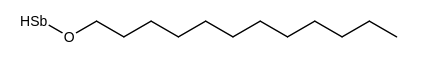
\includegraphics{smile-9a445740653245117b6a4c994fec17ba6c853366}\\
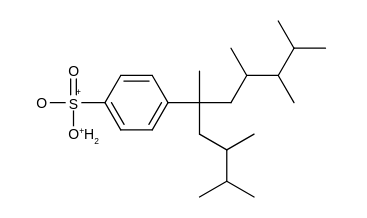
\includegraphics{smile-090c8219ef8a4a90a829b50c8202dd8af7af7ec3}\\
b) Vì sao hiện nay những chất giặt rửa tổng hợp có mạch phân nhánh thường bị cấm sử dụng?\\
2.12. a) Viết công thức khung phân tử của sodium stearate và sodium 4-dodecylbenzenesulfonate.\\
b) So sánh cấu tạo và nguyên tắc làm sạch của 2 chất trên.\\
c) Hãy cho biết khả năng giặt rửa của sodium stearate và sodium 4-dodecylbenzenesulfonate trong nước cứng.\\
2.13. a) Thế nào là chất giặt rửa anion? Vì sao sodium laurylsulfate và sodium 4-dodecylbenzenesulfonate được gọi là các chất giặt rửa anion?\\
b) Giải thích vì sao khi tắm rửa hoặc giặt giũ bằng xà phòng thường thấy xuất hiện các "váng xà phòng", trong khi điều này không xuất hiện khi sử dụng dầu gội đầu, sữa tắm.\\
2.14. Xà phòng hoá hoàn toàn 10 tấn chất béo trung tính $\left(^{(*)}\right.$ cần dùng vừa đủ dung dịch chứa 1680 kg NaOH . Tính khối lượng xà phòng thu được. Cho biết các muối sodium carboxylate trong xà phòng chiếm $65 \%$ khối lượng xà phòng.\\
2.15. Xà phòng hoá hoàn toàn 300 g chất béo A cần dùng vừa đủ 500 mL dung dịch KOH 2 M . Sau phản ứng, sản phẩm thu được gồm muối và $29,44 \mathrm{~g}$ glycerol. Tính khối lượng xà phòng thu được sau phản ứng, cho biết các muối carboxylate trong xà phòng chiếm $70 \%$ khối lượng.\\
2.16. Một nhóm học sinh điều chế xà phòng theo phương pháp đã nêu trong sách giáo khoa Hoá học 12 (Chân trời sáng tạo). Thành phẩm là những bánh xà phòng được nhóm bảo quản nơi thoáng mát, khối lượng ban đầu của mỗi bánh là 100 g . Để hoàn thành báo cáo kết quả thực hành, nhóm đã tiến hành cân khối lượng bánh xà phòng cứ hai ngày một lần và việc này thực hiện liên tục trong vòng 18 ngày, bắt đầu từ ngày tháo khuôn ${ }^{* *}$ ). Kết quả được thể hiện bởi biểu đồ quan hệ giữa cân nặng của bánh xà phòng theo thời gian như sau:

\footnotetext{${ }^{(*)}$ Là chất béo chỉ gồm các triglyceride. Thực tế chất béo còn lẫn một lượng nhỏ các acid béo tự do.\\
(**) Tuỳ khối lượng mẻ xà phòng điều chế, sớm nhất là sau 24 giờ sau khi đổ khuôn.
}
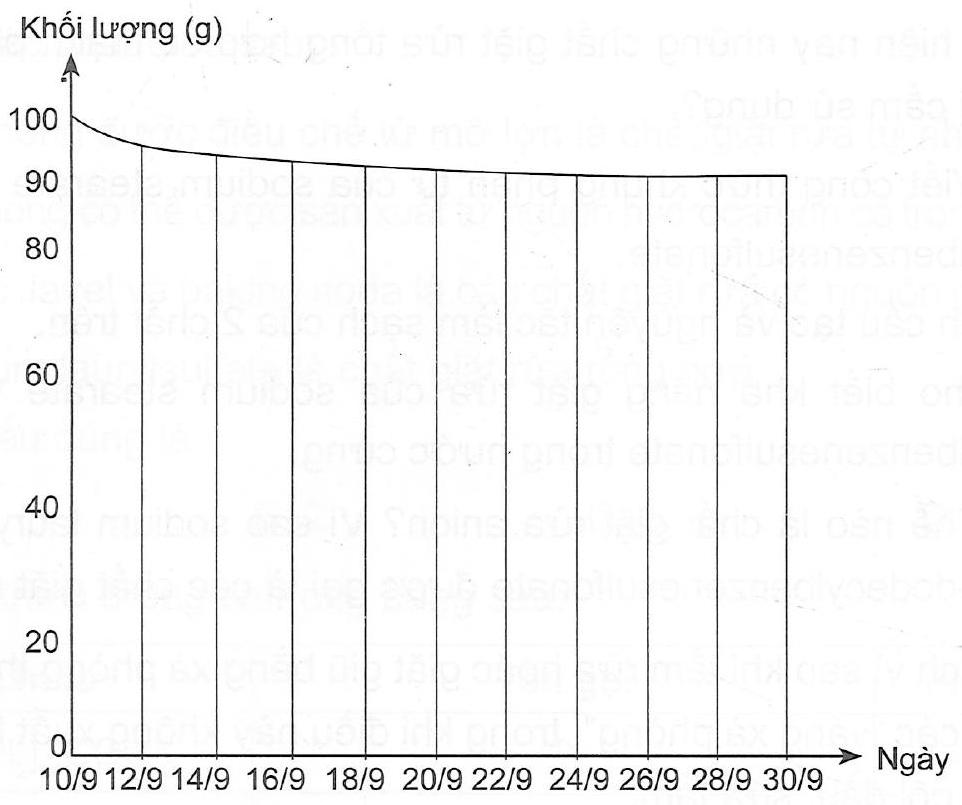
\includegraphics[max width=\textwidth, center]{2025_10_23_de6f5713836e4e91b3c8g-010}

Nhận xét và giải thích kết quả thu được từ biểu đồ của nhóm học sinh trên.\\
2.17. Nước tiểu bình thường có sức căng bề mặt khoảng 66 dyne/cm nhưng nếu có muối mật, nó sẽ giảm xuống còn khoảng 55 dyne/cm. Trong xét nghiệm Hay (Hay's test) giúp phát hiện những người bị bệnh gan như viêm gan, xơ gan, ... bột lưu huỳnh được rắc lên bề mặt nước tiểu. Giải thích cách làm trên.\\
2.18. Từ xa xưa, khi xà phòng và chất giặt rửa còn chưa phổ biến, người ta đã biết sử dụng nước nóng trong giặt giũ sẽ tốt hơn so với nước lạnh. Bằng kiến thức hoá học, em hãy giải thích kinh nghiệm thực tiễn trên.\\
2.19. Giải thích khả năng làm bất hoạt vi khuẩn, virus của xà phòng và chất giặt rửa tổng hợp.\\
2.20. Enzyme là một thành phần thiết yếu của các chất giặt rửa cao cấp và việc sử dụng chúng mang lại cho người tiêu dùng những lợi ích rõ rệt. Những lợi ích này bao gồm khả năng làm việc ở nhiệt độ thấp, tiết kiệm nước, đồng thời loại bỏ nhu cầu sử dụng các hoá chất khắc nghiệt, gây tác động tiêu cực đến môi trường. Ngoài ra, enzyme có thể phân huỷ sinh học nên không để lại dư lượng độc hại.\\
Protease là loại enzyme không thể thiếu trong tất cả các loại hoá chất giặt rửa, nhất là trong bột giặt, do protease thích hợp để dễ loại bỏ các vết bẩn do thức ăn, máu và các dịch do cơ thể con người tiết ra.

Để khảo sát độ hoạt động của protease theo nhiệt độ, người ta tiến hành thí nghiệm nghiên cứu tốc độ phân huỷ chất bẩn bởi protease. Kết quả cho bởi biểu đồ sau:\\
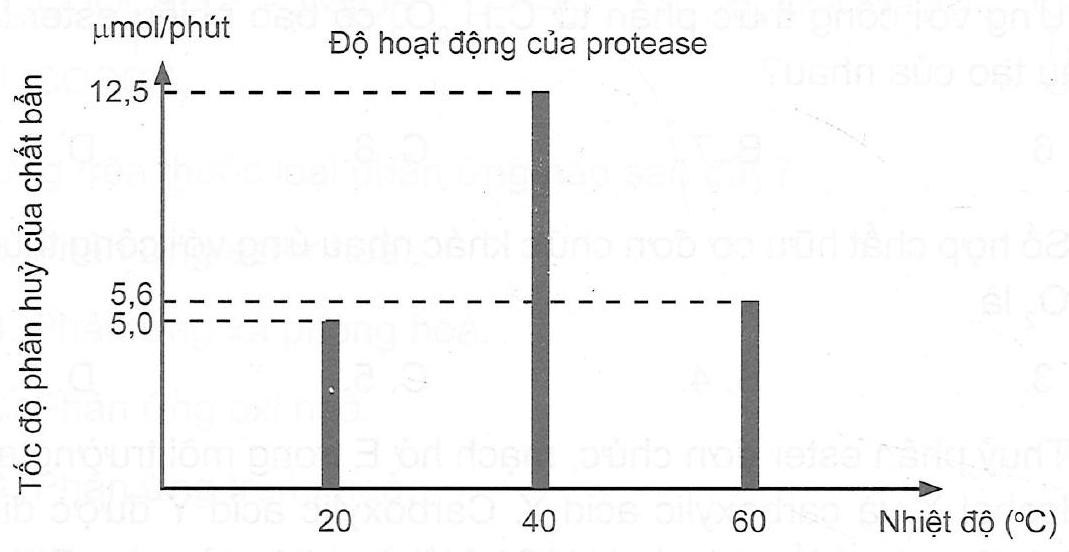
\includegraphics[max width=\textwidth, center]{2025_10_23_de6f5713836e4e91b3c8g-011}

Em hãy cho biết độ hoạt động của protease tối ưu ở nhiệt độ nào trong thí nghiệm trên?\\
2.21. Vì sao không nên sử dụng xà phòng chung với giấm ăn?\\
2.22. Giải thích vai trò dung dịch NaCl bão hoà trong sản xuất xà phòng.\\
2.23. Vì sao chỉ có thể thổi bong bóng với nước xà phòng mà không thể thổi bong bóng với nước sạch?\\
2.24*. Dầu ăn không thể trộn lẫn với nước hoặc giấm hay nước cốt chanh. Tuy nhiên, nếu thêm vào một ít lòng đỏ trứng, chúng sẽ trộn lẫn được với nhau, tạo thành một hỗn hợp gọi là nhũ tương. Lúc này, thêm tiếp một ít gia vị rồi khuấy đều sẽ thu được một loại sốt dùng trong chế biến thực phẩm, giúp tăng hương vị thức ăn và tạo cảm giác ngon miệng.\\
a) Nêu vắn tắt vai trò của lòng đỏ trứng trong quá trình chế biến trên.\\
b) Vì sao lòng đỏ trứng có khả năng giúp trộn lẫn dầu ăn với nước?\\
c) Chất được sử dụng thay thế lòng đỏ trứng ở trên phải có đặc điểm cấu tạo như thế nào?\\
d) Hợp chất sau có được sử dụng để thay thế vai trò của lòng đỏ trứng không? Vì sao?\\
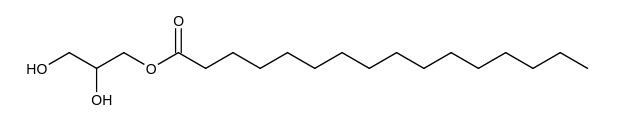
\includegraphics{smile-3e77c415b93edf8952b3a6828d20f7943c672fc5}

glyceryl monopalmitate

\section*{ÔN TÂP CHUONG 1}
OT1.1. Ứng với công thức phân tử $\mathrm{C}_{5} \mathrm{H}_{10} \mathrm{O}_{2}$ có bao nhiêu ester là đồng phân cấu tạo của nhau?\\
A. 6 .\\
B. 7.\\
C. 8 .\\
D. 9 .

OT1.2. Số hợp chất hữu cơ đơn chức khác nhau ứng với công thức phân tử $\mathrm{C}_{4} \mathrm{H}_{8} \mathrm{O}_{2}$ là\\
A. 3 .\\
B. 4 .\\
C. 5.\\
D. 6 .

OT1.3. Thuỷ phân ester đơn chức, mạch hở E trong môi trường acid thu được alcohol X và carboxylic acid Y . Carboxylic acid Y được điều chế bằng cách lên men giấm alcohol $X$. Công thức phân tử ester $E$ là\\
A. $\mathrm{C}_{5} \mathrm{H}_{10} \mathrm{O}_{2}$.\\
B. $\mathrm{C}_{3} \mathrm{H}_{6} \mathrm{O}_{2}$.\\
C. $\mathrm{C}_{4} \mathrm{H}_{6} \mathrm{O}_{2}$.\\
D. $\mathrm{C}_{4} \mathrm{H}_{8} \mathrm{O}_{2}$.

OT1.4. $X, Y, Z$ là 3 chất hữu cơ được kí hiệu ngẫu nhiên trong số các chất $\mathrm{HCOOCH}_{3}, \mathrm{CH}_{3} \mathrm{COOH}$ và $\mathrm{CH}_{3} \mathrm{CH}_{2} \mathrm{CH}_{2} \mathrm{OH}$. Nhiệt độ sôi của $X, Y, Z$ được cho trong bảng sau:

\begin{center}
\begin{tabular}{|l|c|c|c|}
\hline
Chất & $X$ & $Y$ & $Z$ \\
\hline
Nhiệt độ sôi $\left({ }^{\circ} \mathrm{C}\right)$ & 31,8 & 97,0 & 118,0 \\
\hline
\end{tabular}
\end{center}

Các chất $X, Y$ lần lượt là\\
A. $\mathrm{HCOOCH}_{3}$ và $\mathrm{CH}_{3} \mathrm{COOH}$.\\
B. $\mathrm{CH}_{3} \mathrm{COOH}$ và $\mathrm{HCOOCH}_{3}$.\\
C. $\mathrm{CH}_{3} \mathrm{CH}_{2} \mathrm{CH}_{2} \mathrm{OH}$ và $\mathrm{CH}_{3} \mathrm{COOH}$.\\
D. $\mathrm{HCOOCH}_{3}$ và $\mathrm{CH}_{3} \mathrm{CH}_{2} \mathrm{CH}_{2} \mathrm{OH}$.

OT1.5. Ester nào sau đây là đồng phân với methacrylic acid?\\
A. Methyl acrylate.\\
B. Ethyl acrylate.\\
C. Vinyl formate.\\
D. Ethyl acetate.

OT1.6. Cho phản ứng được biểu diễn thông qua phương trình hoá học sau:\\
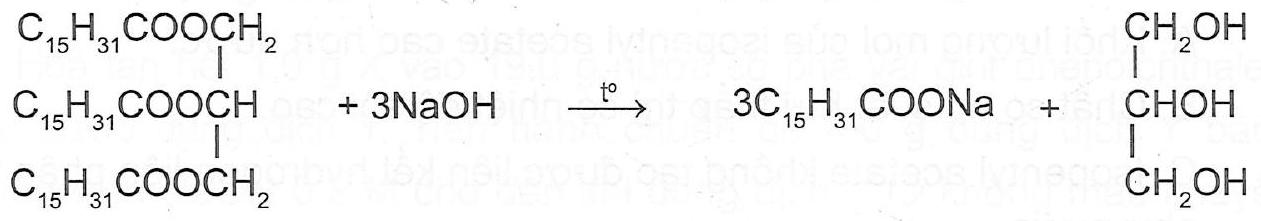
\includegraphics[max width=\textwidth, center]{2025_10_23_de6f5713836e4e91b3c8g-013}

Phản ứng trên thuộc loại phản ứng nào sau đây?\\
A. Phản ứng ester hoá.\\
B. Phản ứng xà phòng hoá.\\
C. Phản ứng oxi hoá.\\
D. Phản ứng trung hoà.

OT1.7. Cho phương trình nhiệt hoá học của các phản ứng sau:

$$
\begin{array}{ll}
2 \mathrm{C}(\mathrm{~s})+\mathrm{O}_{2}(\mathrm{~g})+2 \mathrm{H}_{2}(\mathrm{~g}) \xrightarrow{\mathrm{xt}, \mathrm{t}^{\circ}} \mathrm{HCOOCH}_{3}(\mathrm{l}) & \Delta_{\mathrm{r}} \mathrm{H}_{298}^{\circ}=\mathrm{a} \\
\mathrm{HCOOCH}_{3}(\mathrm{l})+2 \mathrm{O}_{2}(\mathrm{~g}) \xrightarrow{\mathrm{t}^{\circ}} 2 \mathrm{CO}_{2}(\mathrm{~g})+2 \mathrm{H}_{2} \mathrm{O}(\mathrm{~g}) & \Delta_{\mathrm{r}} \mathrm{H}_{298}^{\circ}=\mathrm{b} \\
\mathrm{C}(\mathrm{~s})+\mathrm{O}_{2}(\mathrm{~g}) \xrightarrow{\mathrm{t}^{\circ}} \mathrm{CO}_{2}(\mathrm{~g}) & \Delta_{\mathrm{r}} \mathrm{H}_{298}^{\circ}=\mathrm{c} \\
\mathrm{H}_{2}(\mathrm{~g})+\frac{1}{2} \mathrm{O}_{2}(\mathrm{~g}) \xrightarrow{\mathrm{t}^{\circ}} \mathrm{H}_{2} \mathrm{O}(\mathrm{~g}) & \Delta_{\mathrm{r}} \mathrm{H}_{298}^{\circ}=\mathrm{d}
\end{array}
$$

Mối quan hệ giữa $a, b, c, d$ là\\
A. $a=b+c+d$.\\
B. $a=2 b+c-d$.\\
C. $b=2 a-c+d$.\\
D. $2 d=a+b-2 c$.

OT1.8. Trong điều kiện thường, isopentyl acetate (hay isoamyl acetate) là chất lỏng có mùi thơm của táo và chuối chín.\\
Các thông tin về áp suất hơi(*) ở $25^{\circ} \mathrm{C}$ cùng với nhiệt độ sôi của isopentyl acetate và nước ở điều kiện thường được cho trong bảng sau:

\begin{center}
\begin{tabular}{|c|c|c|}
\hline
Chất & Áp suất hơi ỏ $\mathbf{2 5}{ }^{\circ} \mathrm{C}$ (bar) & Nhiệt độ sôi $\left({ }^{\circ} \mathrm{C}\right)$ \\
\hline
isopentyl acetate & 0,0075 & 142 \\
\hline
nước & 0,0333 & 100 \\
\hline
\end{tabular}
\end{center}

\footnotetext{${ }^{\circ}$ A Áp suất thể hiện bởi hơi xuất hiện trên bề mặt chất lỏng (hoặc rắn) được gọi là áp suất hơi. Một chất lỏng (hoặc rắn) có áp suất hơi cao ở nhiệt độ bình thường được gọi là chất dễ bay hơi. Khi nhiệt độ của chất lỏng (hoặc rắn) tăng, động năng của các phân tử cũng tăng lên, số phân tử chuyển thành thể hơi cũng tăng, do đó áp suất hơi tăng.
}Dữ kiện nào sau đây được dùng để giải thích kết quả đã nêu ở bảng trên?\\
A. Khối lượng mol của isopentyl acetate cao hơn nước.\\
B. Chất có áp suất hơi thấp thì có nhiệt độ sôi cao.\\
C. Isopentyl acetate không tạo được liên kết hydrogen liên phân tử như nước.\\
D. Isopentyl acetate là chất hữu cơ, nước là chất vô cơ.

OT1.9. Trong thí nghiệm điều chế ethyl acetate, bạn học sinh cần đong 24 mL cồn $96^{\circ}$. Dụng cụ nào sau đây phù hợp nhất cho thao tác trên?

\begin{figure}[h]
\begin{center}
\captionsetup{labelformat=empty}
\caption{A.}
  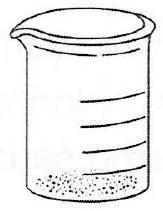
\includegraphics[width=\textwidth]{2025_10_23_de6f5713836e4e91b3c8g-014(2)}
\end{center}
\end{figure}

\begin{figure}[h]
\begin{center}
\captionsetup{labelformat=empty}
\caption{B.}
  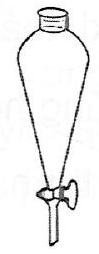
\includegraphics[width=\textwidth]{2025_10_23_de6f5713836e4e91b3c8g-014}
\end{center}
\end{figure}

\begin{figure}[h]
\begin{center}
\captionsetup{labelformat=empty}
\caption{C.}
  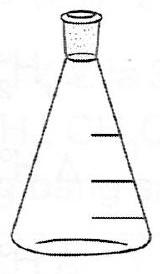
\includegraphics[width=\textwidth]{2025_10_23_de6f5713836e4e91b3c8g-014(3)}
\end{center}
\end{figure}

\begin{figure}[h]
\begin{center}
\captionsetup{labelformat=empty}
\caption{D.}
  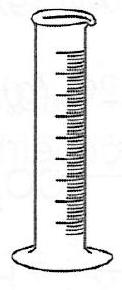
\includegraphics[width=\textwidth]{2025_10_23_de6f5713836e4e91b3c8g-014(1)}
\end{center}
\end{figure}

OT1.10. Một carboxylic acid $X$ có hàm lượng các nguyên tố carbon và hydrogen lần lượt là $40,7 \%$ và $5,1 \%$ về khối lượng.\\
a) Cho biết công thức thực nghiệm của $X$.\\
b) Phổ khối lượng của $X$ có kết quả như hình bên dưới. Xác định công thức phân tử của $X$.\\
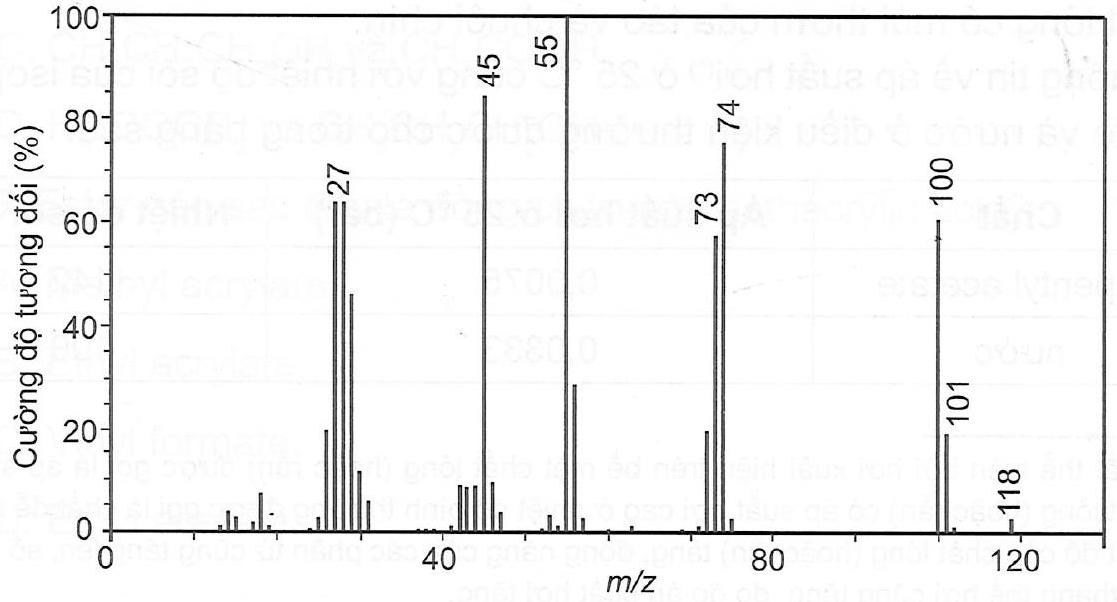
\includegraphics[max width=\textwidth, center]{2025_10_23_de6f5713836e4e91b3c8g-014(4)}\\
c) Viết các công thức cấu tạo có thể có của $X$.\\
d) Hoà tan hết $1,0 \mathrm{~g} \mathrm{X}$ vào $19,0 \mathrm{~g}$ nước có pha vài giọt phenolphthalein thu được dung dịch Y . Tiến hành chuẩn độ $4,0 \mathrm{~g}$ dung dịch Y bằng dung dịch $\mathrm{NaOH} 0,2 \mathrm{M}$ cho đến khi dung dịch Y từ không màu chuyển sang màu hồng nhạt thì dừng lại, thấy đã dùng hết $17,0 \mathrm{~mL}$. Xác định lại phân tử khối của X .\\
e) Đun $X$ với lượng dư ethanol có xúc tác $\mathrm{H}_{2} \mathrm{SO}_{4}$ đặc thu được chất hữu cơ Z chỉ chứa một loại nhóm chức, mạch không phân nhánh. Xác định công thức cấu tạo của $Z$ và viết phương trình hoá học của phản ứng. Gọi tên các chất $X, Z$.\\
g) Đề nghị phương pháp tách chất $Z$ ra khỏi hỗn hợp sau phản ứng.

OT1.11. Oleic acid và elaidic acid là các acid béo đồng phân hình học của nhau, trong đó oleic acid có liên kết đôi $\mathrm{C}=\mathrm{C}$ ở dạng cis và elaidic acid có liên kết đôi $\mathrm{C}=\mathrm{C}$ ở dạng trans.\\
a) Viết công thức khung phân tử của elaidic acid và oleic acid.\\
b) Em có nhận xét gì về cấu trúc phân tử của các acid béo trên.\\
c) So sánh nhiệt độ nóng chảy của oleic acid và elaidic acid. Giải thích.

OT1.12. Hai chất hữu cơ đơn chức, mạch hở $X$ và $Y$ có cùng công thức phân tử $\mathrm{C}_{3} \mathrm{H}_{4} \mathrm{O}_{2}$ với nhiệt độ sôi lần lượt là $47^{\circ} \mathrm{C}$ và $141^{\circ} \mathrm{C}$. Xác định công thức cấu tạo của $\mathrm{X}, \mathrm{Y}$.

OT1.13. Acid béo là thành phần quan trọng của một chế độ ăn uống lành mạnh. Cho biết các acid béo là stearic acid, oleic acid và linoleic acid với công thức khung phân tử được biểu diễn dưới đây:\\
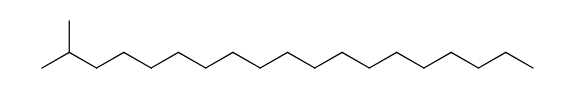
\includegraphics{smile-5d9c0af85b7203517e5ecb36a0446ddb7f1c99ee}

stearic acid\\
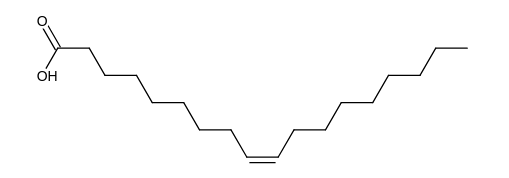
\includegraphics{smile-891fa39fff480eba68434015d30981331f44267a}

oleic acid\\
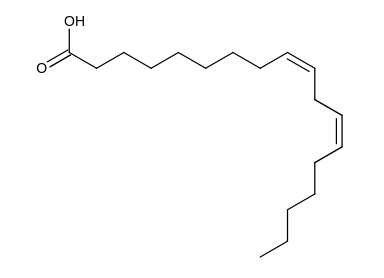
\includegraphics{smile-1a6a5bf79dc94f93de3f3def086c5d6126489e03}

linoleic acid\\
a) Acid béo nào trong số 3 acid nêu trên là acid béo thiết yếu? Vì sao?\\
b) Biết nhiệt độ nóng chảy của các acid béo trên theo thứ tự ngẫu nhiên lần lượt là $-5^{\circ} \mathrm{C}, 13^{\circ} \mathrm{C}$ và $69^{\circ} \mathrm{C}$. Hãy điền các giá trị trên vào bảng theo mẫu sau cho phù hợp và giải thích. Ở điều kiện thường, acid béo nào ở thể lỏng, thể rắn? Giải thích.

\begin{center}
\begin{tabular}{|l|c|c|c|}
\hline
Acid béo & stearic acid & oleic acid & linoleic acid \\
\hline
Nhiệt độ nóng chảy $\left({ }^{\circ} \mathrm{C}\right)$ & $?$ & $?$ & $?$ \\
\hline
\end{tabular}
\end{center}

c) Giải thích vì sạo muối sodium hoặc potassium của chúng được sử dụng làm xà phòng.\\
OT1.14. Vì sao một số loài chim có thể dễ dàng bơi lội, thậm chí ngụp lặn dưới nước để săn mồi nhưng lại bị chết chìm bởi các vết dầu loang?

OT1.15. Theo em, đầu ưa nước của một phân tử xà phòng có công thức RCOONa là -COONa hay $-\mathrm{COO}^{-}$. Vì sao?

OT1.16. Sáp Carnauba là một loại sáp thực vật thu được từ lá cây cọ Carnauba ở Brazil. Sáp Carnauba có thành phần chính là myricyl cerotate, một ester tạo bởi myricyl alcohol có công thức là $\mathrm{CH}_{3}\left[\mathrm{CH}_{2}\right]_{29} \mathrm{OH}$ và cerotic acid là một acid béo có công thức $\mathrm{CH}_{3}\left[\mathrm{CH}_{2}\right]_{24} \mathrm{COOH}$. Sáp Carnauba được sử dụng rộng rãi để đánh bóng sàn nhà, ô tô, đồ nội thất, ...\\
a) Viết công thức khung phân tử của myricyl cerotate.\\
b) Theo em, lớp sáp phủ trên lá của cây có tác dụng gì?

OT1.17. Linolenic acid có công thức phân tử là $\mathrm{C}_{18} \mathrm{H}_{30} \mathrm{O}_{2}$, gồm có $\alpha$-linolenic acid và $\gamma$-linolenic acid. $\alpha$-linolenic acid là một acid béo có 3 liên kết đôi cùng dạng cis ở các vị trí $9,12,15$ tính từ nguyên tử carbon của nhóm carboxyl, còn $\gamma$-linolenic acid là một acid béo cũng có 3 liên kết đôi cùng dạng cis ở các vị trí $6,9,12$ tính từ nguyên tử carbon của nhóm carboxyl.\\
a) Viết công thức khung phân tử của $\alpha$-linolenic acid và $\gamma$-linolenic acid.\\
b) Chúng có phải là các acid béo thiết yếu không? Vì sao?\\
c) So sánh nhiệt độ nóng chảy của mỗi acid trên với stearic acid. Giải thích.

OT1.18. a) Nguyên nhân nào dẫn đến việc ôi thiu và bốc mùi của các chất béo nếu chúng không được bảo quản cẩn thận?\\
b) Vì sao bơ để lâu ngoài không khí thường xuất hiện mùi khó ngửi?\\
c) Giải thích sự hình thành malondialdehyde (MDA), một hợp chất có công thức cấu tạo $\mathrm{CH}_{2}(\mathrm{CHO})_{2}$. Hợp chất này có khả năng gây ung thư và có mùi khó chịu khi các chất béo có chứa thành phần là linoleic acid hoặc linolenic acid bị oxi hoá.\\
d) Nêu nguyên tắc hoạt động của chất chống oxi hoá trong việc giúp bảo quản chất béo.\\
e) Trình bày một số tác hại của việc sử dụng dầu, mỡ ôi thiu.

Trong mỗi ý a), b), c), d) ở mỗi câu OT1.19 đến OT1.22, học sinh chọn đúng hoặc sai.\\
OT1.19. Phổ khối lượng của ester E được cho dưới đây:\\
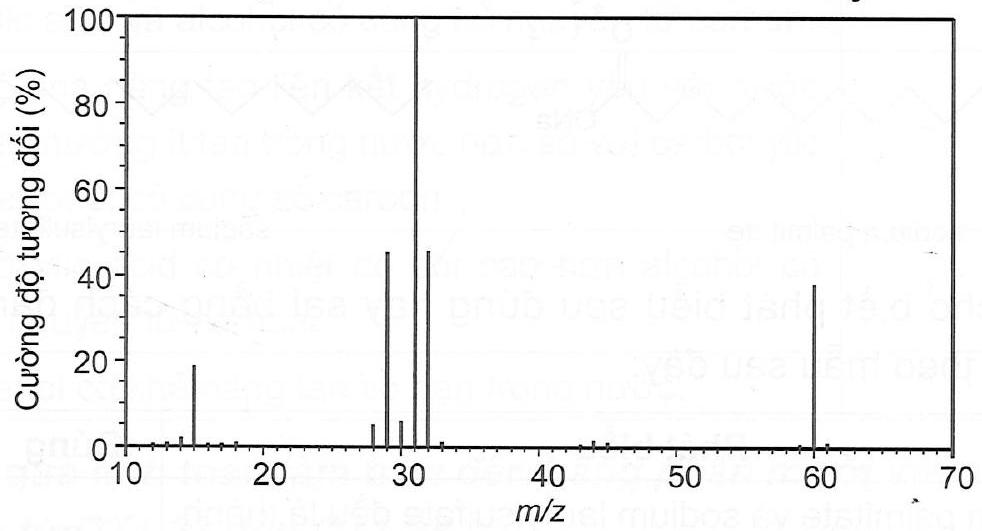
\includegraphics[max width=\textwidth, center]{2025_10_23_de6f5713836e4e91b3c8g-017}

Em hãy cho biết phát biểu sau đúng hay sai bằng cách đánh dấu $\checkmark$ vào bảng theo mẫu sau đây:

\begin{center}
\begin{tabular}{|l|c|c|}
\hline
\multicolumn{1}{|c|}{Phát biểu} & Đúng & Sai \\
\hline
a) Ester E có khối lượng phân tử là $\mathrm{M}=60$. & $?$ & $?$ \\
\hline
b) E là ester của methyl alcohol. & $?$ & $?$ \\
\hline
\end{tabular}
\end{center}

\begin{center}
\begin{tabular}{|l|l|l|}
\hline
c) Nhiệt độ sội của E cao hơn ethyl alcohol. & ? & ? \\
\hline
\begin{tabular}{l}
d) Xà phòng hoá E bằng dung dịch NaOH thu được muối \\
có công thức $\mathrm{CHO}_{2} \mathrm{Na}$. \\
\end{tabular} & ? & ? \\
\hline
\end{tabular}
\end{center}

OT1.20. Cho các triglyceride $X, Y$ với công thức cấu tạo sau:

\begin{figure}[h]
\begin{center}
  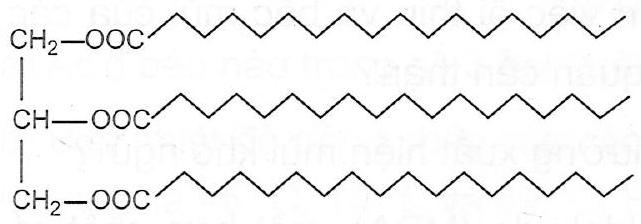
\includegraphics[width=\textwidth]{2025_10_23_de6f5713836e4e91b3c8g-018(1)}
\captionsetup{labelformat=empty}
\caption{triglyceride X}
\end{center}
\end{figure}

\begin{figure}[h]
\begin{center}
  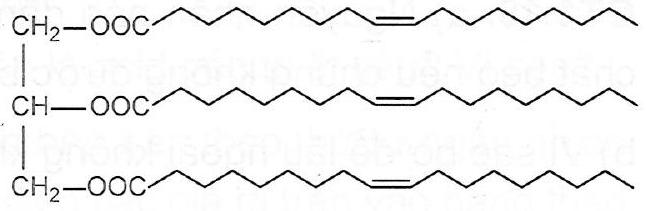
\includegraphics[width=\textwidth]{2025_10_23_de6f5713836e4e91b3c8g-018}
\captionsetup{labelformat=empty}
\caption{triglyceride Y}
\end{center}
\end{figure}

Em hãy cho biết phát biểu sau đúng hay sai bằng cách đánh dấu vào bảng theo mẫu sau đây:

\begin{center}
\begin{tabular}{|l|l|l|}
\hline
Phát biểu & Đúng & Sai \\
\hline
a) Triglyceride $X$ có tên gọi là tripalmitin. & ? & ? \\
\hline
b) X là chất béo no, Y là chất béo không no. & ? & ? \\
\hline
c) $X, Y$ đều tan tốt trong nước. & ? & ? \\
\hline
d) Hydrogen hoá $Y$ thu được $X$. & ? & ? \\
\hline
\end{tabular}
\end{center}

OT1.21. Cho các chất sau:\\
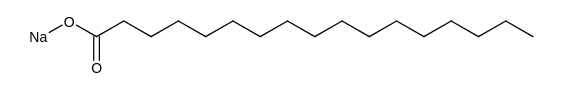
\includegraphics{smile-ff11e193a516b262283bdf1ceb23158362d25710}

sodium palmitate\\
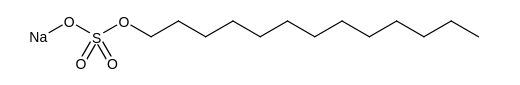
\includegraphics{smile-fd5a9847228aad44f40de606561d8caea432c97b}

sodium laurylsulfate

Em hãy cho biết phát biểu sau đúng hay sai bằng cách đánh dấu $\checkmark$ vào bảng theo mẫu sau đây:

\begin{center}
\begin{tabular}{|l|c|c|}
\hline
\multicolumn{1}{|c|}{Phát biểu} & Đúng & Sai \\
\hline
\begin{tabular}{l}
a) Sodium palmitate và sodium laurylsulfate đều là thành \\
phần chính của xà phòng. \\
\end{tabular} & $?$ & $?$ \\
\hline
\begin{tabular}{l}
b) Sodium palmitate và sodium laurylsulfate đều có tính \\
năng giặt rửa. \\
\end{tabular} & $?$ & $?$ \\
\hline
\begin{tabular}{l}
c) Sodium palmitate và sodium laurylsulfate đều tạo muối \\
khó tan trong nước cứng. \\
\end{tabular} & $?$ & $?$ \\
\hline
\end{tabular}
\end{center}

d) Sodium palmitate và sodium laurylsulfate đều có đầu ưa nước gắn với đuôi kị nước.

\begin{center}
\begin{tabular}{|l|l|}
\hline
$?$ & $?$ \\
\hline
\end{tabular}
\end{center}

OT1.22. Nhiệt độ sôi và độ tan của một số ester, carboxylic acid và alcohol có cùng số nguyên tử carbon được cho trong bảng sau:

\begin{center}
\begin{tabular}{|l|l|l|}
\hline
Công thức & Nhiệt độ sôi ( ${ }^{\circ} \mathrm{C}$ ) & Độtan ơ $2^{\circ} \mathrm{C}$ ( $\mathrm{g} / 100 \mathrm{~g} \mathrm{nước}$ ) \\
\hline
$\mathrm{HCOOCH}_{3}$ & 31,5 & 23,0 \\
\hline
$\mathrm{HCOOC}_{2} \mathrm{H}_{5}$ & 54,2 & 12,0 \\
\hline
$\mathrm{CH}_{3} \mathrm{COOH}$ & 117,9 & Tan vô hạn \\
\hline
$\mathrm{C}_{2} \mathrm{H}_{5} \mathrm{COOH}$ & 141 & Tan vô hạn \\
\hline
$\mathrm{C}_{2} \mathrm{H}_{5} \mathrm{OH}$ & 78,4 & Tan vô hạn \\
\hline
$\mathrm{CH}_{3} \mathrm{CH}_{2} \mathrm{CH}_{2} \mathrm{OH}$ & 97,2 & Tan vô hạn \\
\hline
\end{tabular}
\end{center}

Em hãy cho biết phát biểu sau đúng hay sai bằng cách đánh dấu $\checkmark$ vào bảng theo mẫu sau đây:

\begin{center}
\begin{tabular}{|l|l|l|}
\hline
Phát biểu & Đúng & Sai \\
\hline
a) Do không tạo được liên kết hydrogen giữa các phân tử nên ester có nhiệt độ sôi thấp hơn nhiệt độ sôi của carboxylic acid và alcohol có cùng số nguyên tử carbon. & ? & ? \\
\hline
b) Do có khả năng tạo liên kết hydrogen yếu với nước nên ester thường ît tan trong nước hơn so với carboxylic acid và alcohol có cùng số carbon. & ? & ? \\
\hline
c) Carboxylic acid có nhiệt độ sôi cao hơn alcohol có cùng số nguyên tử carbon. & ? & ? \\
\hline
d) Methanol có khả năng tan vô hạn trong nước. & ? & ? \\
\hline
\end{tabular}
\end{center}

Các kết quả tính toán làm tròn đến hàng phần mười với các câu trả lời ngắn từs OT1.23 đến OT1.28.

OT1.23. Có bao nhiêu ester của methyl alcohol có công thức phân tử là $\mathrm{C}_{5} \mathrm{H}_{10} \mathrm{O}_{2}$ ?\\
OT1.24. Có bao nhiêu hợp chất hữu cơ đơn chức, phân tử chỉ chứa carbon, hydrogen, oxygen và có phân tử khối là 60 ?

OT1.25. Có bao nhiêu triglyceride mà khi xà phòng hoá hoàn toàn thu được glycerol cùng hỗn hợp chỉ gồm muối của palmitic acid và stearic acid?

OT1.26. Xà phòng hoá hoàn toàn $0,1 \mathrm{~mol}$ ester E đơn chức, mạch hở bằng dung dịch NaOH vừa đủ thu được muối F và alcohol G . Biết khối lượng muối F thu được lớn hơn khối lượng ester E đã tham gia xà phòng hoá. Tính khối lượng alcohol G thu được.

OT1.27. Xà phòng hoá hoàn toàn một ester mạch hở E (chỉ tạo bởi một carboxylic acid và một alcohol) bằng lượng vừa đủ dung dịch NaOH rồi cô cạn, thu được muối khan F và alcohol G . Đốt cháy hoàn toàn F chỉ thấy tạo $\mathrm{CO}_{2}$ và $0,2 \mathrm{~mol} \mathrm{Na}_{2} \mathrm{CO}_{3}$, còn đốt cháy hoàn toàn G được số mol $\mathrm{H}_{2} \mathrm{O}$ gấp hai lần số $\mathrm{mol} \mathrm{CO}_{2}$. Xác định khối lượng của E , cho biết phân tử khối của $\mathrm{E}<200$.

OT1.28. Trong thực tế, thành phần chất béo gồm các triglyceride có lẫn một ît acid béo tự do. Để sản xuất được m gam xà phòng, người ta thuỷ phân hoàn toàn 300 g chất béo A trong 500 mL dung dịch KOH 2 M (vừa đủ). Sau phản ứng thu được $29,44 \mathrm{~g}$ glycerol. Xác định giá trị của m . Cho biết các muối carboxylate trong xà phòng chiếm $70 \%$ khối lượng xà phòng. Khối lượng KOH đã dùng để xà phòng hoá là tổng khối lượng KOH tác dụng với acid béo tự do và KOH tác dụng với các triglyceride.

\section*{GLUCOSE VÀ FRUCTOSE}
3.1. Chất nào sau đây không thuộc nhóm hợp chất carbohydrate?\\
A. Tinh bột.\\
B. Glucosamine.\\
C. Fructose.\\
D. Glucose.\\
3.2. Phát biểu nào sau đây không đúng về glucose và fructose?\\
A. Chúng đều có công thức phân tử $\mathrm{C}_{6} \mathrm{H}_{12} \mathrm{O}_{6}$.\\
B. Chúng đều là các hợp chất carbohydrate.\\
C. Chúng đều là các monosaccharide.\\
D. Chúng có tính chất hoá học tương tự nhau.\\
3.3. Trong các phát biểu sau đây, phát biểu nào không đúng?\\
A. Glucose và fructose là hai đồng phân cấu tạo.\\
B. Saccharose và maltose là hai đồng phân cấu tạo.\\
C. Tinh bột và cellulose là hai đồng phân cấu tạo.\\
D. Glucose, fructose, saccharose, maltose, tinh bột và cellulose đều là các carbohydrate.\\
3.4. Carbohydrate nào sau đây là thành phần chính của mật ong?\\
A. Glucose.\\
B. Maltose.\\
C. Saccharose.\\
D. Fructose.\\
3.5. Cho các phát biểu sau về glucose và fructose:\\
(1) Glucose và fructose là hai đồng phân lập thể.\\
(2) Fructose còn được gọi là đường trái cây và là carbohydrate tự nhiên có vị ngọt nhất.\\
(3) Glucose là carbohydrate mà cơ thể sử dụng làm nhiên liệu.\\
(4) Người mắc bệnh đái tháo đường có lượng glucose trong máu cao hơn mức bình thường.\\
Số phát biểu đúng là\\
A. 1.\\
B. 2.\\
C. 3 .\\
D. 4 .\\
3.6. Hormone nào sau đây làm giảm lượng glucose trong máu?\\
A. Adrenaline.\\
B. Thyroxine.\\
C. Insuline.\\
D. Oxytocine.\\
3.7. Tuyến nội tiết nào sau đây giữ cho nồng độ glucose trong máu ổn định?\\
A. Tuyến yên.\\
B. Tuyến tuy.\\
C. Tuyến thượng thận.\\
D. Tuyến giáp.\\
3.8. Nồng độ glucose trong máu là $6 \mathrm{mmol} / \mathrm{L}$ có nghĩa 1 dL máu chứra bao nhiêu mg glucose?\\
A. 1080,0 .\\
B. 108,0 .\\
C. 10800,0 .\\
D. 10,8 .

Đồ thị sau đây biểu diễn sụp thay đổi về lượng glucose trong máu của một người sử dụng đồ uống có đường sau 8 giò nhịn ăn:\\
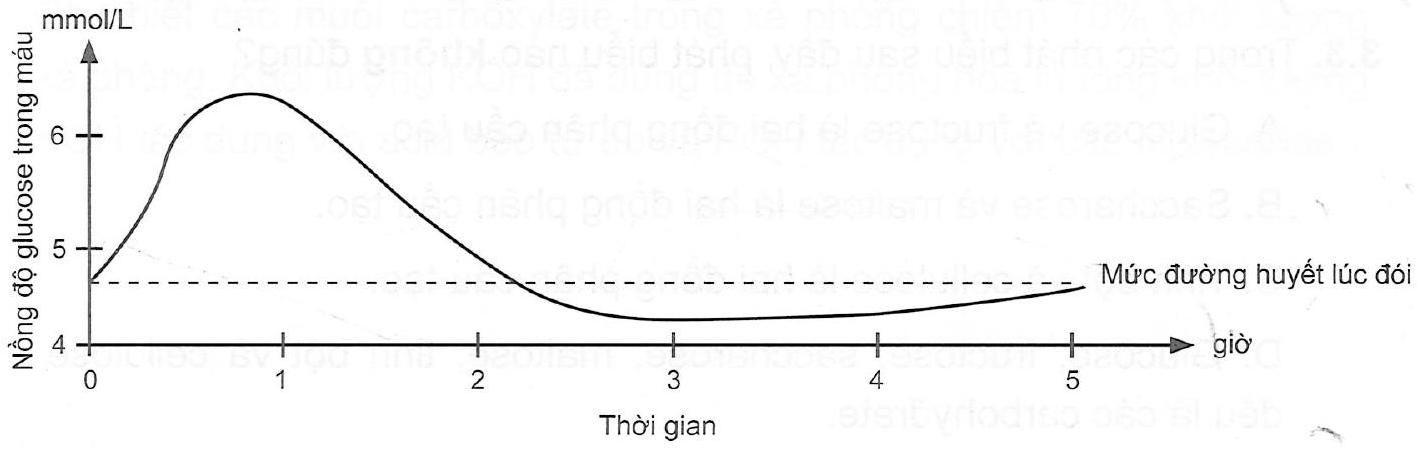
\includegraphics[max width=\textwidth, center]{2025_10_23_de6f5713836e4e91b3c8g-022}

Sử dụng đồ thị trên để trả lời các câu 3.9 và 3.10 .\\
3.9. Khi sử dụng đồ uống có đường, nồng độ glucose trong máu tăng cao nhất sau khi\\
A. sử dụng khoảng 20 phút.\\
B. sử dụng khoảng 2 giờ.\\
C. sử dụng khoảng 50 phút.\\
D. sử dụng khoảng 3 giờ.\\
3.10. Chỉ số đường huyết của một người lúc đói được đo khi chưa ăn hay uống bất kì loại thực phẩm nào ít nhất trong 8 giờ. Khi chỉ số đường huyết lúc đói đạt dưới $100 \mathrm{mg} / \mathrm{dL}$ thì bình thường, từ $126 \mathrm{mg} / \mathrm{dL}$ trở lên thì có khả năng mắc bệnh đái tháo đường. Lúc này cần tiếp tục kiểm tra đường huyết bằng thử nghiệm dung nạp glucose qua đường uống. Sau 2 giờ, nhân viên y tế sẽ lấy máu để xét nghiệm tiếp. Nếu đường huyết dưới $140 \mathrm{mg} / \mathrm{dL}$ thì bình thường, từ 140 đến $199 \mathrm{mg} / \mathrm{dL}$ bị tiền đái tháo đường và từ' $200 \mathrm{mg} / \mathrm{dL}$ trở lên là bị đái tháo đường ${ }^{()}$.

Biểu diễn lại đồ thị đã cho theo $\mathrm{mg} / \mathrm{dL}$ glucose. Dựa vào đồ thị biểu diễn đường huyết này, em hãy cho biết tình trạng sức khoẻ người được khảo sát trên đồ thị.\\
3.11. Trong một thử nghiệm y tế để đo khả năng dung nạp carbohydrate của cơ thể người, một người trưởng thành được cho uống dung dịch glucose $20 \%$. Đối với một trẻ nhỏ, nồng độ glucose phải được giảm xuống còn $10 \%$. Cần dùng bao nhiêu gam dung dịch glucose $20 \%$ và bao nhiêu gam nược để pha được 8 g dung dịch glucose $10 \%$ ?\\
3.12. Chỉ số đường huyết của bạn Thành và bạn Nhân được đo 3 lần trong một tuần. Kết quả được ghi nhận ở bảng sau:

\begin{center}
\begin{tabular}{|c|c|c|c|}
\hline
\multirow{2}{*}{} & \multicolumn{3}{|c|}{Chỉ số đường huyết (mg/dL)} \\
\cline { 2 - 4 }
 & Lần 1 & Lần 2 & Lần 3 \\
\hline
Bạn Thành & 80 & 80 & 83 \\
\hline
Bạn Nhân & 60 & 95 & 115 \\
\hline
\end{tabular}
\end{center}

a) Chỉ số đường huyết trung bình của mỗi bạn là bao nhiêu?\\
b) Độ lệch chuẩn cho mỗi kết quả là bao nhiêu?\\
c) Bạn nào có kết quả đường huyết tốt hơn? Giải thích?

\footnotetext{(*) \href{https://tamanhhospital.vn/xet-nghiem-tieu-duong/}{https://tamanhhospital.vn/xet-nghiem-tieu-duong/}
}
3.13. Đề nghị phương pháp hoá học phân biệt 3 lọ dung dịch mất nhãn chứa glucosé, fructose và glycerol.\\
3.14. Độ tan trong nước của glucose ở $25^{\circ} \mathrm{C}$ là 91 g trong 100 g nước và ở $50^{\circ} \mathrm{C}$ là 244 g trong 100 g nước. Khối lượng glucose kết tinh thu được khi làm lạnh 172 g dung dịch glucose bão hoà ở $50^{\circ} \mathrm{C}$ xuống $25^{\circ} \mathrm{C}$ là bao nhiêu? Giả thiết khi làm lạnh, sự bay hơi nước xảy ra không đáng kể.\\
3.15. Tiến hành ether hoá $\alpha$-glucose bằng methanol, sản phẩm thu được là methyl $\alpha$-glucoside ${ }^{(*)}$ theo phương trình phản ứng sau:\\
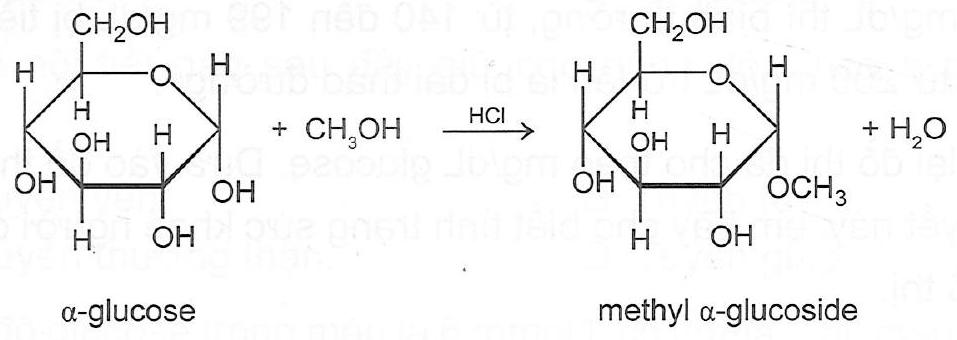
\includegraphics[max width=\textwidth, center]{2025_10_23_de6f5713836e4e91b3c8g-024}

Methyl $\alpha$-glucoside có phản ứng với thuốc thử Tollens không? Vì sao?\\
$3.16^{*}$. So sánh độ bền của $\alpha$-glucose với $\beta$-glucose. Giải thích.\\
Biểu đồ dưới đây biểu diễn lượng đường huyết trước, trong và sau quá trình tập thể dục của một người khoẻ mạnh, không mắc bệnh đái tháo đường.\\
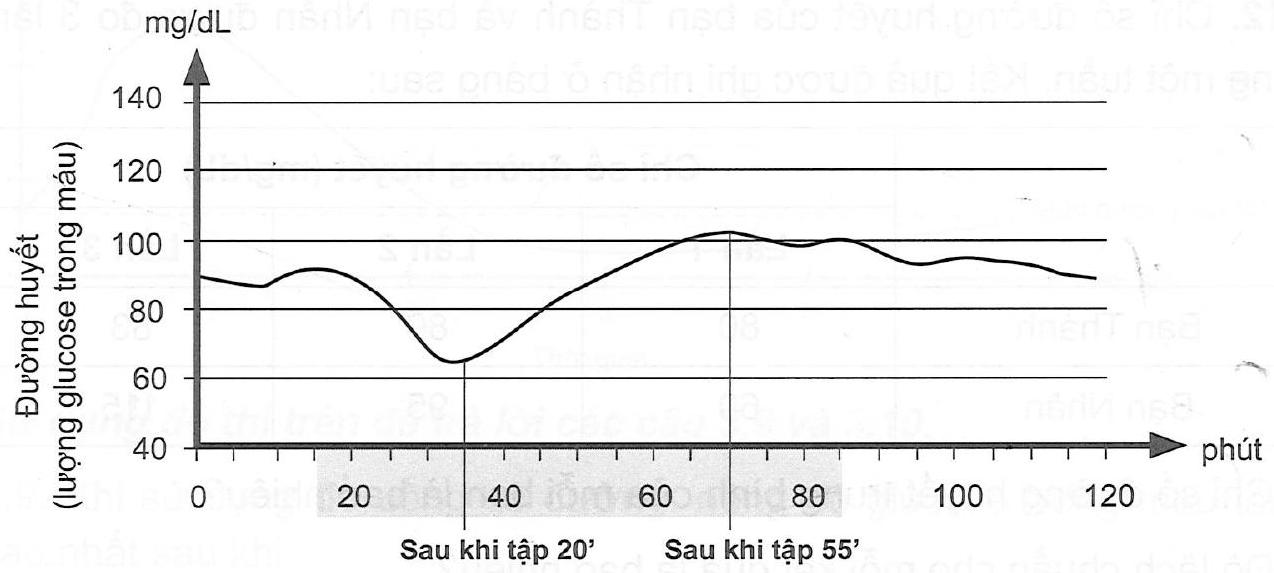
\includegraphics[max width=\textwidth, center]{2025_10_23_de6f5713836e4e91b3c8g-024(1)}\\
$\Delta$ Biểu đồ đường huyết theo thời gian (phần tô màu là thời gian tập thể dục)\\
Sử dụng thông tin từ biểu đồ trên để trả lời các câu 3.17 và 3.18 .

\footnotetext{${ }^{(7)}$ Ngoài methyl $\alpha$-glucoside, còn thu được methyl $\beta$-glucoside.
}
3.17. Sau khi quan sát biểu đồ trên, có các phát biểu sau:\\
a) Quá trình tập thể dục diễn ra trong khoảng 70 phút.\\
b) Lượng đường huyết giảm khi bắt đầu tập thể dục và xuống mức thấp nhất sau 20 phút tập.\\
c) Lượng đường huyết tăng lên mức cao nhất sau khi tập thể dục được 55 phút.\\
d) Sau khi tập thể dục xong, lượng đường huyết có xu hướng giảm.

Có bao nhiêu phát biểu trong số các phát biểu trên là đúng? Giải thích.\\
3.18. Nêu nhận xét và giải thích sự thay đổi lượng đường huyết trong, sau quá trình tập thể dục.\\
3.19*. Ester của glucose với acid béo là các chất hoạt động bề mặt không ion, không độc và có khả năng phân huỷ sinh học. Chúng đóng vai trò là chất nhũ hoá, chất giặt rửa, chất làm ẩm, chất tạo bọt, ... trong các ngành công nghiệp mĩ phẩm, thực phẩm, nông nghiệp và dược phẩm.

Ester của glucose và acid béo được tổng hợp dựa trên quá trình ester hoá ở nhiệt độ cao với sự có mặt của chất xúc tác cùng các dung môi hữu cơ. Điều này làm cho môi trường trở nên độc hại do các hoá chất này không dễ phân huỷ sinh học. Vấn đề trên có thể khắc phục bằng cách sử dụng những chất xúc tác sinh học như enzyme lipase với các điều kiện phản ứng nhẹ nhàng và mức tiêu thụ năng lượng ít hơn, giúp tránh tình trạng biến tính của các chất phản ứng và sản phẩm. Ngoài ra, enzyme này cũng có thể mang lại tính chọn lọc cao dẫn đến hiệu suất phản ứng cao.

Viết phương trình hoá học của phản ứng điều chế ester sau từ các chất tương ứng (xúc tác candida antarctica lipase B, CALB(*)).\\
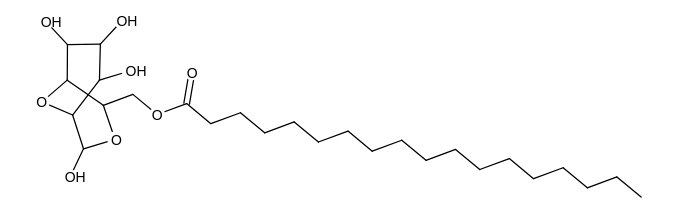
\includegraphics{smile-dad72375a16e7b0ca5e51835a7586b2c504c2672}

\footnotetext{${ }^{(*)}$ CALB là enzyme chính trong công nghệ sinh học, được tạo thành từ 317 gốc amino acid, phân tử khối là 33273.
}4

\section*{SACCHAROSE VÀ MALTOSE}
Cho 4 carbohydrate sau: glucose, fructose, maltose, saccharose.\\
Nhận định các carbohydrate trên để trả lời các câu 4.1, 4.2, 4.3, 4.4, 4.5 và 4.6.\\
4.1. Có bao nhiêu carbohydrate đã cho thuộc nhóm disaccharide?\\
A. 1 .\\
B. 2 .\\
C. 3 .\\
D. 4 .\\
4.2. Số carbohydrate đã cho có liên kết $\alpha-1,4$-glycoside trong phân tử là\\
A. 1.\\
B. 2 .\\
C. 3 .\\
D. 4 .\\
4.3. Số carbohydrate đã cho có liên kết $\alpha-1,2-$ glycoside trong phân tử là\\
A. 1.\\
B. 2 .\\
C. 3 .\\
D. 4 .\\
4.4. Carbohydrate nào sau đây có cấu trúc phân tử không đổi ở trạng thái rắn hoặc trong dung dịch?\\
A. Glucose.\\
B. Fructose.\\
C. Saccharose.\\
D. Maltose.\\
4.5. Cấu trúc phân tử của carbohydrate nào trong nhóm nêu trên không có nhóm - OH hemiacetal hoặc hemiketal?\\
A. Glucose.\\
B. Fructose.\\
C. Saccharose.\\
D. Maltose.\\
4.6. Trong số các carbohydrate đã nêu, số carbohydrate có khả năng mở vòng cho xuất hiện trở lại các nhóm aldehyde (-CHO) hoặc ketone ( $>C=O$ ) là\\
A. 1 .\\
B. 2.\\
C. 3 .\\
D. 4 .\\
4.7. Mạch nha là tên gọi khác của carbohydrate nào sau đây?\\
A. Glucose.\\
B. Fructose.\\
C. Saccharose.\\
D. Maltose.\\
4.8. Thuỷ phân 100 g saccharose thu được $103,6 \mathrm{~g}$ hỗn hợp $X$ gồm glucose, fructose và saccharose còn dư. Hiệu suất thuỷ phân saccharose đạt\\
A. $100 \%$.\\
B. $68,4 \%$.\\
C. $95 \%$.\\
D. $57 \%$.\\
4.9. Thuỷ phân 57 g maltose thu được 57 g glucose. Hiệu suất thuỷ phân maltose thành glucose đạt\\
A. $100 \%$.\\
B. $50 \%$.\\
C. $95 \%$.\\
D. $57 \%$.\\
4.10. Giải thích vì sao saccharose chỉ tồn tại một kiểu cấu trúc phân tử ở trạng thái rắn hoặc trong dung dịch.\\
4.11. Thế nào là đường khử? Trong số các carbohydrate gồm glucose, fructose, saccharose và maltose, carbohydrate nào là đường khử? Carbohydrate nào không phải là đường khử? Giải thích.\\
4.12. Giải thích vì sao maltose bị khử bởi $\mathrm{NaBH}_{4}$ nhưng saccharose không cho phản ứng này?\\
4.13. Đường nghịch chuyển (invert sugar) ${ }^{(*)}$ là hỗn hợp gồm các lượng như nhau của fructose và glucose, được tạo ra từ quá trình thuỷ phân saccharose. Trong đời sông, đường nghịch chuyển được điều chế ở dạng siro. Loại đường này được sử dụng rộng rãi trong sản xuất thực phẩm, đồ uống do có khả năng giữ nước cùng với có vị ngọt cao hơn từ $20 \%-25 \%$ so với saccharose, mang lại hương vị mới, hữu ích cho sản phẩm. Ví dụ đường nghịch chuyển có khả năng giữ ẩm tốt hơn saccharose giúp sản phẩm nướng giữ được độ tươi và màu vỏ đẹp, tăng độ mềm cho các món nướng; bánh kẹo nhờ đó được bộ sung độ ẩm, không bị khô nhanh. Đường nghịch chuyển cũng giúp siro không có hiện tượng kết tinh lại đường, tạo độ mịn cho các sản phẩm như kem, giúp giảm điểm đóng băng của kem, nhờ đó kem không bị xuất hiện các vảy đá khi bảo quản, ...

\footnotetext{${ }^{(*)}$ Gọi là đường nghịch chuyển vì nó phản xạ ánh sáng theo hướng ngược lại so với đường saccharose: saccharose xoay ánh sáng phân cực sang phải trong khi đường nghịch chuyển quay ánh sáng phân cực sang trái.
}Để sản xuất đường nghịch chuyển, người ta tiến hành đun sôi nhẹ dung dịch saccharose trong chảo lớn với xúc tác citric acid để làm giảm pH dung dịch xuống 1,6 . Ba yếu tố này dẫn đến việc saccharose bị thuỷ phân thành glucose và fructose. Cuối cùng, dùng $\mathrm{NaHCO}_{3}$ để trung hoà citric acid sau phản ứng.\\
a) Viết phương trình hoá học của các phản ứng xảy ra khi điều chế đường nghịch chuyển từ saccharose.\\
b) Giải thích vì sao đường nghịch chúyển tự động xuất hiện trong quá trình sản xuất mứt.\\
c) Từ 10 tấn saccharose có thể thu được tối đa bao nhiêu tấn đường nghịch chuyển?\\
4.14. Đường nghịch chuyển thật sự có nhiều lợi ích so với đường saccharose, tức đường mía quen thuộc tại nhà như đã trình bày ở bài trên. Em có thể sản xuất đường nghịch chuyển từ đường saccharose sẵn có tại nhà theo hướng dẫn sau:

\section*{Thí nghiệm: Điều chế đường nghịch chuyển từs saccharose}
Dụng cụ: cân, ống đong, nhiệt kế, nồi thuỷ tinh hoặc inox, bếp.\\
Hoá chất: nước, saccharose, 5 quả chanh tươi.

\section*{Tiến hành:}
Bước 1: Cho vào nồi 480 mL nước. Thêm tiếp 1 kg đường cát và nước cốt chanh. Khuấy đều cho đường tan hết.\\
Bước 2: Đun sôi nhẹ dung dịch thu được trong khoảng 1 giờ. Thỉnh thoảng khuấy đều.

Khi nhiệt độ đường trong nồi đạt khoảng $1.14^{\circ} \mathrm{C}$, công đoạn điều chế đã hoàn tất. Có thể kiểm tra bằng cách cho một ít đường vào nước lạnh, đường thành phẩm phải cuộn lại thành khối.\\
Bước 3: Tắt bếp, để đường nguội đến nhiệt độ phòng. Thành phẩm sẽ đặc như siro, có thể trữ trong các lọ thuỷ tinh để dùng dần.\\
a) Vì sao dùng đường nghịch chuyển trong pha chế thực phẩm kinh tế hơn so với việc dùng đường saccharose?\\
b) Viết báo cáo thực hành theo mẫu sau:\\
I. Mục tiêu\\
II. Nguyên liệu, dụng cụ, hoá chất\\
III. Cách tiến hành\\
IV. Thảo luận, đánh giá kết quả

\begin{itemize}
  \item Về màu.
  \item Về mùi.
  \item Về độ sánh.
  \item Về khả năng tan trong nước.\\
V. Kết luận\\
4.15*. Saccharose monolaurate là ester thu được khi cho saccharose tác dụng với lauric acid.\\
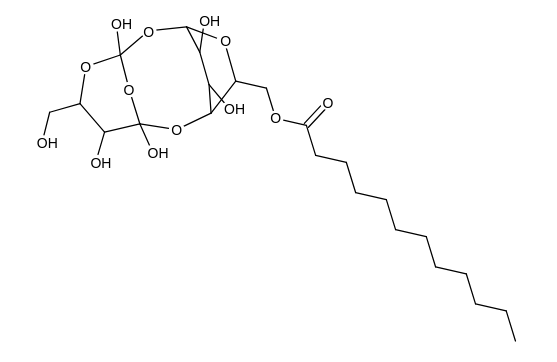
\includegraphics{smile-6ed5beaea46dc16ce0749d12d7229229ff6ce397}
\end{itemize}

saccharose monolaurate\\
a) Cho biết công thức phân tử của saccharose monolaurate.\\
b) Vì sao saccharose monolaurate được sử dụng làm chất nhũ hoá?\\
c) Saccharose monolaurate có phản ứng với thuốc thử Tollens không? Giải thích.\\
d) Saccharose monolaurate là một trong những chất phụ gia có chức năng kép do khả năng nhũ hoá và hoạt tính kháng khuẩn của nó. Từ 500 g saccharose và 100 g lauric acid có thể điều chế được tối đa bao nhiêu gam saccharose monolaurate? Cho biết hiệu suất phản ứng đạt $47 \%$.\\
4.16. Vì sao glucose được dùng để truyền tĩnh mạch trong y học, trong khi không thể sử dụng saccharose?\\
4.17*. a) Giải thích vì sao đường được sử dụng trong bảo quản thực phẩm.\\
b) Giữa glucose và saccharose, loại đường nào thích hợp hơn trong việc bảo quản thực phẩm? Giải thích.

\section*{Brit \\
 5}
\section*{TINH BỘT VÀ CELLULOSE}
Cho 4 carbohydrate sau: saccharose, maltose, tinh bột và cellulose. Nhận định các carbohydrate trên để trả lời các câu 5.1, 5.2, 5.3 và 5.4.\\
5.1. Có bao nhiêu carbohydrate đã cho thuộc nhóm polysaccharide?\\
A. 2 .\\
B. 3 .\\
C. 4 .\\
D. 5 .\\
5.2. Số carbohydrate đã cho có liên kết $\alpha-1,4-$ glycoside trong phân tử là\\
A. 1 .\\
B. 2 .\\
C. 3 .\\
D. 4 .\\
5.3. Số carbohydrate đã cho có liên kết $\alpha-1,4-$ glycoside trong phân tử là\\
A. 1 .\\
B. 2 .\\
C. 3 .\\
D. 4 .\\
5.4. Số carbohydrate đã cho có thể có liên kết $\alpha-1,6-$ glycoside trong phân tử là\\
A. 1 .\\
B. 2.\\
C. 3 .\\
D. 4 .\\
5.5. Carbohydrate nào có cấu trúc phân tử được biểu diễn dưới đây?\\
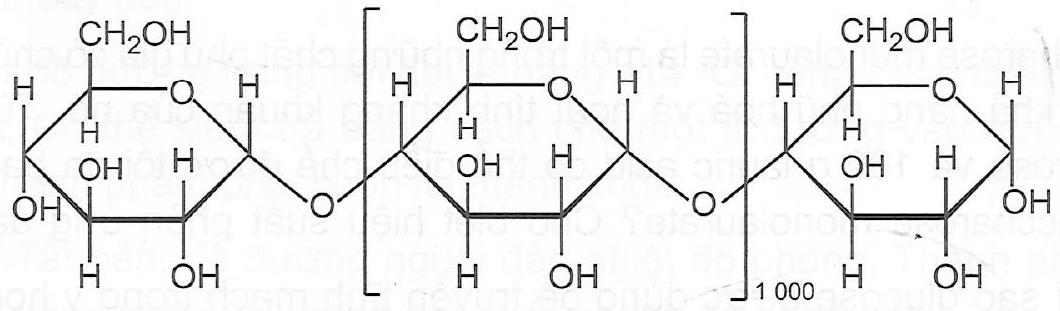
\includegraphics[max width=\textwidth, center]{2025_10_23_de6f5713836e4e91b3c8g-030}\\
A. Saccharose.\\
B. Cellulose.\\
C. Maltose.\\
D. Amylose.\\
5.6. Quan sát cấu trúc phân tử carbohydrate $X$ được cho dưới đây:\\
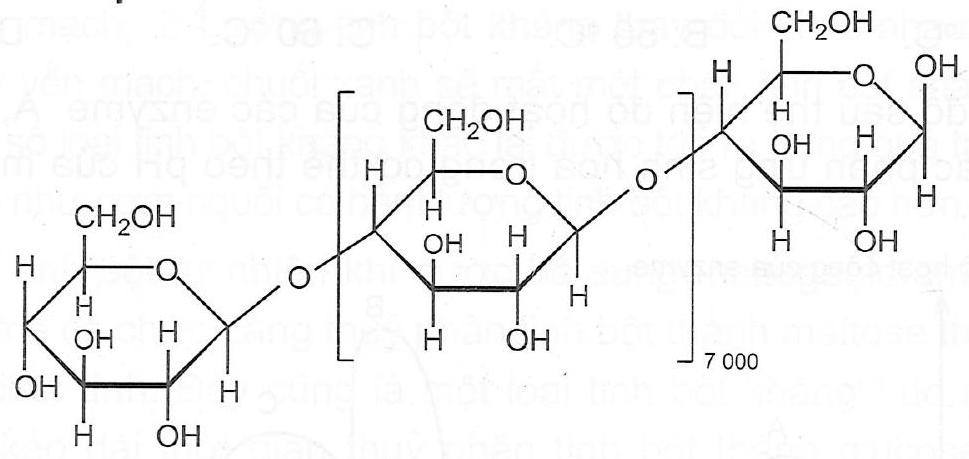
\includegraphics[max width=\textwidth, center]{2025_10_23_de6f5713836e4e91b3c8g-031}

Phát biểu nào sau đây là đúng về carbohydrate $X$ ?\\
A. $X$ có nhiều trong trái cây chín.\\
B. $X$ chỉ có cấu trúc mạch không phân nhánh.\\
C. $X$ có vị ngọt hơn glucose.\\
D. $X$ là thành phần chính của các loại hạt như ngô, gạo, đậu, ...\\
5.7. Trong số 6 carbohydrate sau: glucose, fructose, saccharose, maltose, tinh bột và cellulose. Số carbohydrate cho được phản ứng thuỷ phân là\\
A. 2 .\\
B. 3 .\\
C. 4 .\\
D. 5 .\\
5.8. Hầu hết những phản ứng sinh hoá xảy ra nhờ sự xúc tác của các enzyme. Biểu đồ dưới đây thể hiện tốc độ của một phản ứng sinh hoá do enzyme $X$ làm xúc tác theo nhiệt độ:\\
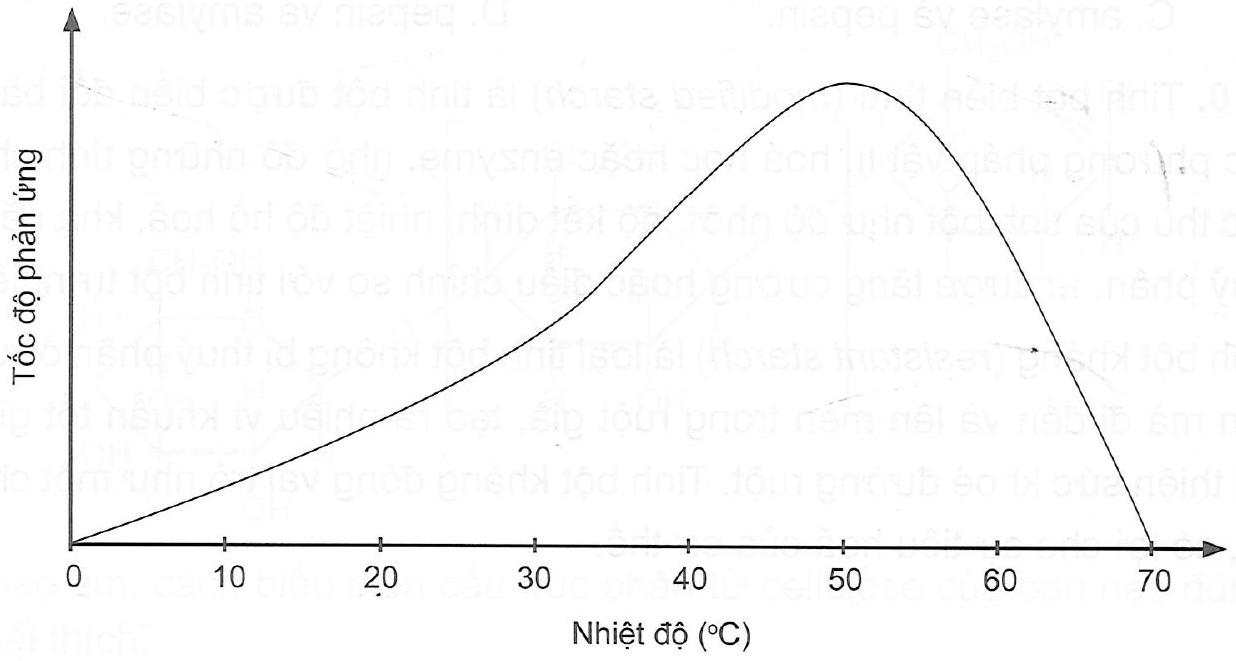
\includegraphics[max width=\textwidth, center]{2025_10_23_de6f5713836e4e91b3c8g-031(1)}

Nhiệt độ tối ưu cho enzyme $X$ hoạt động là\\
A. $0^{\circ} \mathrm{C}$.\\
B. $50^{\circ} \mathrm{C}$.\\
C. $60^{\circ} \mathrm{C}$.\\
D. $70^{\circ} \mathrm{C}$.\\
5.9. Biểu đồ sau thể hiện độ hoạt động của các enzyme A, B, C xúc tác cho các phản ứng sinh hoá trong cơ thể theo pH của môi trường phản ứng:

\begin{figure}[h]
\begin{center}
\captionsetup{labelformat=empty}
\caption{Độ hoạt động của enzyme}
  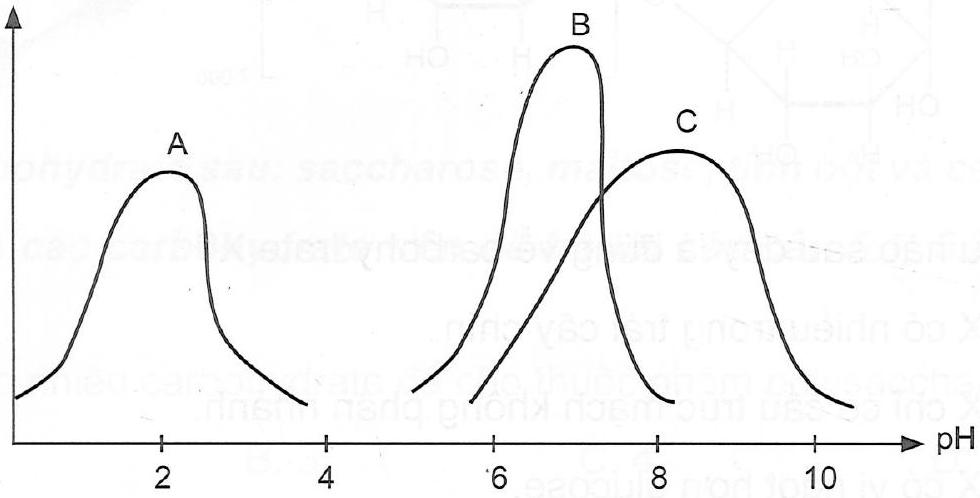
\includegraphics[width=\textwidth]{2025_10_23_de6f5713836e4e91b3c8g-032}
\end{center}
\end{figure}

Trong số các enzyme đã nêu trong biểu đồ, amylase là một enzyme tiêu hoá chủ yếu được tiết ra bởi tuyến tuỵ và tuyến nước bọt, có tác dụng thuỷ phân tinh bột thành maltose. Pepsin và trypsin cũng là các enzyme tiệu hoá, lần lượt có trong dịch vị và ruột non với vai trò phân giải protein. Trypsin hoạt động tốt nhất trong môi trường kiềm nhẹ.\\
Enzyme $A$ và $B$ lần lượt là\\
A. amylase và trypsin.\\
B. pepsin và trypsin.\\
C. amylase và pepsin.\\
D. pepsin và amylase.\\
5.10. Tinh bột biến tính (modified starch) là tinh bột được biến đổi bằng các phương pháp vật lí, hoá học hoặc enzyme, nhờ đó những tính chất đặc thù của tinh bột như độ nhớt, độ kết dính, nhiệt độ hồ hoá, khả năng thuỷ phân, ... được tăng cường hoặc điều chỉnh so với tinh bột tụ nhiên. Tinh bột kháng (resistant starch) là loại tinh bột không bị thuỷ phân ở ruột non mà đi đến và lên men trong ruột già, tạo ra nhiều vi khuẩn tốt giúp cải thiện sức khoẻ đường ruột. Tinh bột kháng đóng vai trò như một chất xơ, có lợi cho sự tiêu hoá của cơ thể.

Tinh bột kháng xuất hiện tự nhiên trong một số loại thực phẩm như chuối xanh, yến mạch, ... Lượng tinh bột kháng thay đổi khác nhau theo nhiệt độ, vì vậy yến mạch, chuối xanh sẽ mất một phần tinh bột kháng khi nấu chín. Một số loại tinh bột kháng khác lại được tạo ra trong quá trình nấu và làm nguội như cơm nguội có hàm lượng tinh bột kháng cao hơn cơm nóng. Ngoài ra, tinh bột tự nhiên khi được bổ sung maltogenic amylase, một loại enzyme có chức năng thuỷ phân tinh bột thành maltose thì thu được tinh bột biến tính. Đây cũng là một loại tinh bột kháng ${ }^{(*)}$ do maltogenic amylase kéo dài thời gian thuỷ phân tinh bột thành glucose giúp làm chậm quá trình tiêu hoá.\\
a) Cho biết vai trò của tinh bột kháng đối với sức khoẻ của cơ thể.\\
b) Em hãy đề nghị cách đơn giản nhất để tăng lượng tinh bột kháng trong khẩu phần ăn hằng ngày.\\
5.11. Trong giờ học, Thành và Nhân lần lượt biểu diễn cấu trúc phân tử cellulose như sau:\\
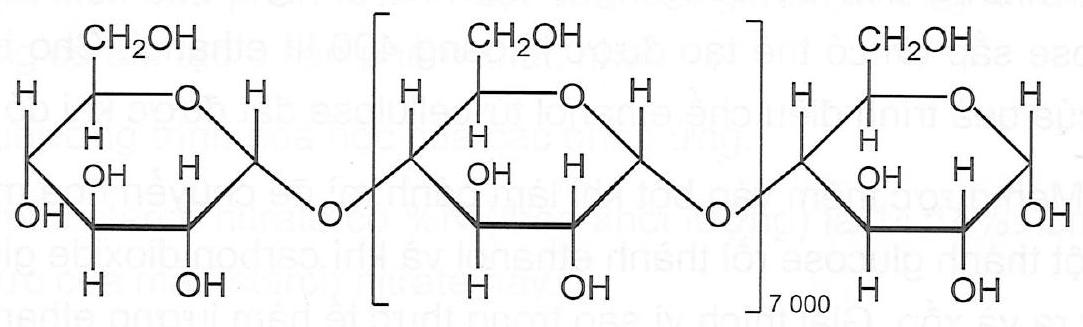
\includegraphics[max width=\textwidth, center]{2025_10_23_de6f5713836e4e91b3c8g-033}\\
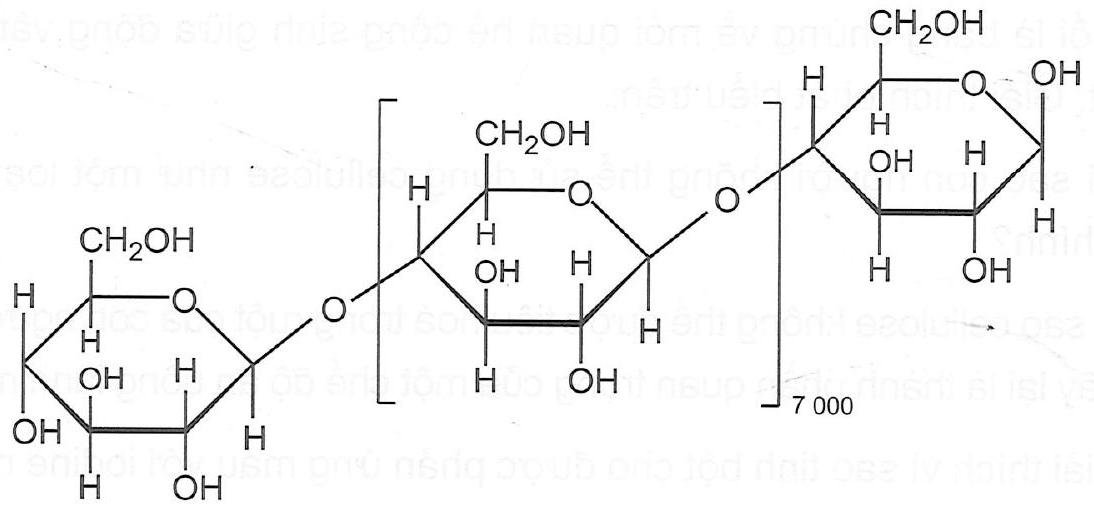
\includegraphics[max width=\textwidth, center]{2025_10_23_de6f5713836e4e91b3c8g-033(1)}

Theo em, cách biểu diễn cấu trúc phân tử cellulose của bạn nào đúng? Giải thích.

\footnotetext{${ }^{(7)}$ Nguồn: \href{https://hopkinsdiabetesinfo.org/what-is-resistant-starch/}{https://hopkinsdiabetesinfo.org/what-is-resistant-starch/}
}
5.12. Ngô và mía là hai nguyên liệu chính được sử dụng trong sản xuất ethanol. Tuy nhiên chúng là những loại cây lương thực quan trọng, trong khi cellulose cũng có thể sản xuất ethanol, nhưng cellulose là nguồn nguyên liệu dồi dào, dễ tìm. Tuy giá thành sản xuất ethanol từ cellulose còn cao, xuất phát từ loại nấm được nuôi cấy để tạo cellulase là enzyme xúc tác cho phản ứng thuỷ phân cellulose thành glucose còn tốn kém nhiều về năng lượng, nhưng hướng đi này đang hứa hẹn nhiều viễn cảnh mới ở tương lai ${ }^{\mathrm{e}}$.\\
a) Viết phương trình hoá học của các phản ứng điều chế ethanol từ cellulose.\\
b) Hiện tại, 1 tấn nguyên liệu cellulose khô tạo ra khoảng 240 lít ethanol. Tính hiệu suất của quá trình điều chế. Cho khối lượng riêng của ethanol là $0,79 \mathrm{~g} / \mathrm{mL}$.\\
c) Với những tiến bộ công nghệ đạt được, người ta tin rằng 1 tấn cellulose sắp tới có thể tạo được khoảng 400 lít ethanol. Cho biết hiệu suất của quá trình điều chế ethanol từ cellulose đạt được khi đó.\\
5.13. Mèn được thêm vào bột khi làm bánh mì để chuyển hoá một phần tinh bột thành glucose rồi thành ethanol và khí carbon dioxide giúp bánh mì nở ra và xốp. Giải thích vì sao trong thực tế hàm lượng ethanol trong bánh mì rất thấp?\\
5.14. Mối là bằng chứng về mối quan hệ cộng sinh giữa động vật và vi sinh vật. Giải thích phát biểu trên.\\
5.15. Vì sao con người không thể sử dụng cellulose như một loại thực phẩm chính?\\
5.16. Vì sao cellulose không thể được tiêu hoá trong ruột của con người, tuy nhiên đây lại là thành phần quan trọng của một chế độ ăn uống lành mạnh?\\
5.17. Giải thích vì sao tinh bột cho được phản ứng màu với iodine nhưng cellulose không cho phản ứng này?

\footnotetext{(*) Nguồn: \href{http://large.stanford.edu}{http://large.stanford.edu}.
}
5.18. Quan sát cấu trúc một phân tử tinh bột dưới đây, ta thấy mỗi phân tử tinh bột có chửa một nhóm -OH hemiacetal có thể mở vòng tạo nhóm aldehyde. Tuy nhiên thực tế tinh bột không phản ứng với thuốc thử Tollens. Giải thích.\\
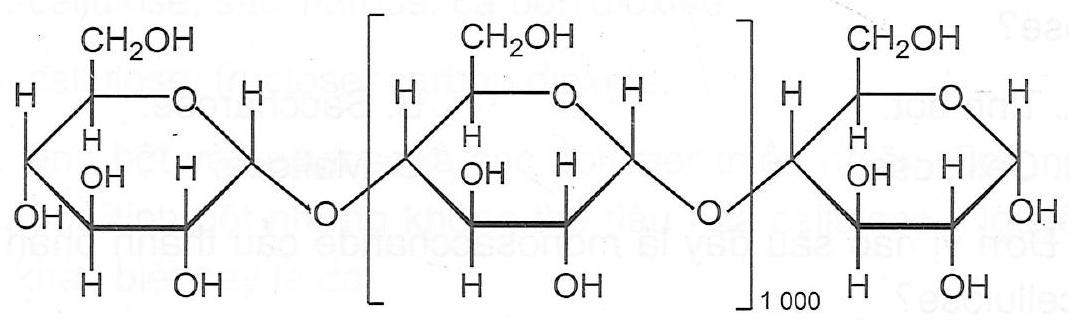
\includegraphics[max width=\textwidth, center]{2025_10_23_de6f5713836e4e91b3c8g-035}\\
5.19. Starch nitrate là một loại bột vô định hình màu vàng nhạt, được tạo thành khi nitrate hoá tinh bột tương tự như nitrate hoá cellulose. Starch nitrate từng được sử dụng trong sản xuất lựu đạn và chất nổ trong khai thác quặng. Cũng giống như cellulose, tuỳ thuộc vào số nhóm -OH trong mắt xích của phân tử tinh bột đã tham gia phản ứng nitrate hoá, phản ứng có thể tạo 3 sản phẩm khác nhau.\\
a) Viết phương trình hoá học của các phản ứng.\\
b) Một mẫu starch nitrate có $\% \mathrm{~N}$ (theo khối lượng) là $14,14 \%$. Cho biết công thức của mẫu starch nitrate này.\\
5.20. Vì sao chỉ tiêu thụ tinh bột nhưng cơ thể vẫn có thể mắc bệnh béo phì?

\section*{ÔN TÂP CHUONG 2}
OT2.1. Carbohydrate nào sau đây không được tạo thành chỉ từ các đơn vị glucose?\\
A. Tinh bột.\\
B. Saccharose.\\
C. Cellulose.\\
D. Maltose.

OT2.2. Đơn vị nào sau đây là monosaccharide cấu thành phân tử tinh bột và cellulose?\\
A. Fructose.\\
B. Maltose.\\
C. Saccharose.\\
D. Glucose.

OT2.3. Glucose được tìm thấy trong tự nhiên dưới dạng D-glucose hoặc L-glucose ${ }^{(*)}$, trong đó D-glucose có nhiều trong tự nhiên còn L-glucose ít gặp hơn. Dextrose là tên gọi khác của D-glucose. Phát biểu nào sau đây không đúng về dextrose?\\
A. Dextrose là một carbohydrate.\\
B. Dextrose và glucose có cùng công thức phân tử.\\
C. Dextrose phản ứng được với thuốc thử Tollens.\\
D. Do không thể mở vòng, dextrose không có cấu tạo dạng mạch hở.

OT2.4. Cho sơ đồ phản ứng:\\
(a) $X+\mathrm{H}_{2} \mathrm{O} \xrightarrow{x t} Y$\\
(b) $\mathrm{Y}+\left[\mathrm{Ag}\left(\mathrm{NH}_{3}\right)_{2}\right] \mathrm{OH} \xrightarrow{\mathrm{t}^{\circ}}$ ammonium gluconate $+\mathrm{Ag}+\mathrm{NH}_{3}+\mathrm{H}_{2} \mathrm{O}$\\
(c) $Y \xrightarrow{x t} E+Z$\\
(d) $Z+\mathrm{H}_{2} \mathrm{O} \xrightarrow[\text { chất diệp lục }]{\text { ánh sáng }} X+G$

\footnotetext{(*) D-glucose và L-glucose là các đồng phân quang học, trong đó D-glucose quay ánh sáng phân cực phẳng theo chiều kim đồng hồ, còn L-glucose quay ánh sáng phân cực phẳng ngược chiều kim đồng hồ.
}Các chất $X, Y, Z$ lần lượt là:\\
A. tinh bột, glucose, ethanol.\\
B. tinh bột, glucose, carbon dioxide.\\
C. cellulose, saccharose, carbon dioxide.\\
D. cellulose, fructose, carbon dioxide.

OT2.5. Tinh bột và cellulose là các polymer thiên nhiên. Con người có thể tiêu hoá tinh bột nhưng không thể tiêu hoá cellulose. Nguyên nhân của sự khác biệt này là do\\
A. số đơn vị mắt xích trong các phân tử tinh bột và cellulose là khác nhau.\\
B. phần trăm khối lượng carbon trong cellulose lớn hơn so với tinh bột.\\
C. cách liên kết giữa các đơn vị mắt xích ở mỗi loại phân tử.\\
D. phân tử cellulose không phân nhánh.

OT2.6. Chất nào sau đây không phải polymer sinh học?\\
A. Tinh bột.\\
B. Cellulose.\\
C. Glucosamine.\\
D. Chitin.

OT2.7. Trong quá trình lên men một carbohydrate, biểu đồ nào dưới đây thể hiện tốt nhất vai trò xúc tác của enzyme cho sự hình thành sản phẩm $P$ theo thời gian?

\begin{figure}[h]
\begin{center}
\captionsetup{labelformat=empty}
\caption{A.}
  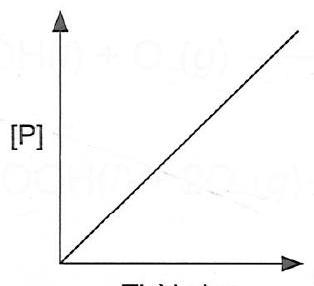
\includegraphics[width=\textwidth]{2025_10_23_de6f5713836e4e91b3c8g-037(1)}
\end{center}
\end{figure}

Thời gian

\begin{figure}[h]
\begin{center}
\captionsetup{labelformat=empty}
\caption{B.}
  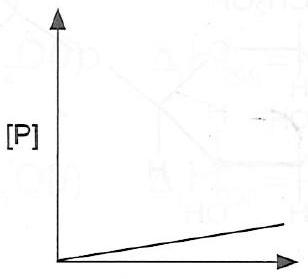
\includegraphics[width=\textwidth]{2025_10_23_de6f5713836e4e91b3c8g-037}
\end{center}
\end{figure}

\begin{figure}[h]
\begin{center}
\captionsetup{labelformat=empty}
\caption{C.}
  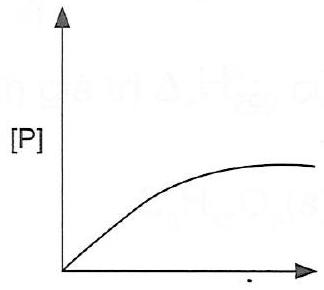
\includegraphics[width=\textwidth]{2025_10_23_de6f5713836e4e91b3c8g-037(2)}
\end{center}
\end{figure}

Thời gian

\begin{figure}[h]
\begin{center}
\captionsetup{labelformat=empty}
\caption{D.}
  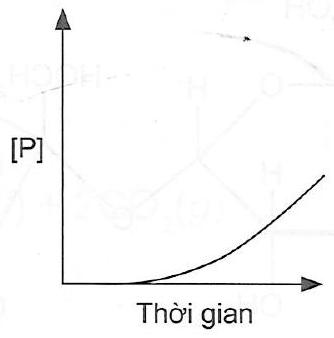
\includegraphics[width=\textwidth]{2025_10_23_de6f5713836e4e91b3c8g-037(3)}
\end{center}
\end{figure}

OT2.8. Đốt cháy hoàn toàn hỗn hợp $X$ gồm glucose, saccharose và tinh bột thu được $8,8 \mathrm{~g} \mathrm{CO}_{2}$ và $3,24 \mathrm{~g}$ nước. Khối lượng hỗn hợp X đã đốt là\\
A. $12,04 \mathrm{~g}$.\\
B. $2,76 \mathrm{~g}$.\\
C. $7,68 \mathrm{~g}$.\\
D. $5,64 \mathrm{~g}$.

OT2.9. Cho các phát biểu sau về carbohydrate:\\
a) Saccharose và fructose không phải là đường khử.\\
b) Amylopectin phân nhánh là do sự xuất hiện của liên kết $\alpha-1,6$-glycoside.\\
c) Cellulose không phân nhánh do chỉ xuất hiện liên kết $\beta$-1,4-glycoside.\\
d) Số nhóm -OH trong phân tử saccharose là 8 .

Số phát biểu đúng là\\
A. 1 .\\
B. 2 .\\
C. 3 .\\
D. 4 .

OT2.10. Giải thích vì sao các phân tử glucose, fructose và maltose đều có thể mở vòng nhưng phân tử saccharose lại không có khả năng này.\\
OT2.11. Thế nào là liên kết glycoside? Cho ví dụ.\\
OT2.12. Cho biết tên của loại liên kết giữa 2 đơn vị monosaccharide đã nêu trong các chuỗi mắt xích hoặc phân tử sau:\\
a)\\
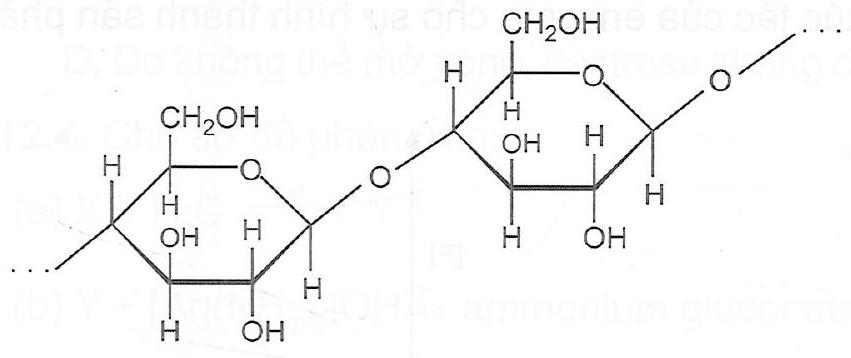
\includegraphics[max width=\textwidth, center]{2025_10_23_de6f5713836e4e91b3c8g-038}\\
b)\\
\includegraphics[max width=\textwidth, center]{2025_10_23_de6f5713836e4e91b3c8g-038(1)}\\
c)\\
\includegraphics[max width=\textwidth, center]{2025_10_23_de6f5713836e4e91b3c8g-039}\\
d)\\
\includegraphics[max width=\textwidth, center]{2025_10_23_de6f5713836e4e91b3c8g-039(1)}

OT2.13. Khi ăn, carbohydrate được chuyển thành glucose. Glucose theo máu đi đến các tế bào rồi bị oxi hoá để tạo ra năng lượng nuôi cơ thể, còn carbon dioxide và nước thì carbon dioxide được thải qua đường thở. Tịnh thể tích carbon dioxide được thải ra khi 60 g glucose bị oxi hoá. Cho biết ở nhiệt độ cơ thể người bình thường, $1 \mathrm{~mol} \mathrm{CO}_{2}$ có thể tích 25,4 lít. Hiệu suất phản ứng đạt 100\%.

OT2.14. Cho phương trình nhiệt hoá học các phản ứng sau:\\
$\mathrm{C}_{2} \mathrm{H}_{5} \mathrm{OH}(l)+\mathrm{O}_{2}(g) \xrightarrow{\mathrm{t}^{\circ}} \mathrm{CH}_{3} \mathrm{COOH}(l)+\mathrm{H}_{2} \mathrm{O}(l) \quad \Delta_{r} \mathrm{H}_{298}^{\circ}=-492,6 \mathrm{~kJ}$\\
$\mathrm{CH}_{3} \mathrm{COOH}(l)+2 \mathrm{O}_{2}(g) \xrightarrow{\mathrm{t}^{\circ}} 2 \mathrm{CO}_{2}(g)+2 \mathrm{H}_{2} \mathrm{O}(l) \quad \Delta_{r} \mathrm{H}_{298}^{\circ}=-874,2 \mathrm{~kJ}$\\
$\mathrm{C}_{6} \mathrm{H}_{12} \mathrm{O}_{6}(\mathrm{~s})+6 \mathrm{O}_{2}(\mathrm{~g}) \xrightarrow{\mathrm{t}^{\circ}} 6 \mathrm{CO}_{2}(\mathrm{~g})+6 \mathrm{H}_{2} \mathrm{O}(\mathrm{l}) \quad \Delta_{\mathrm{r}} \mathrm{H}_{298}^{\circ}=-2805,0 \mathrm{~kJ}$\\
Tính giá trị $\Delta_{\mathrm{r}} \mathrm{H}_{298}^{\circ}$ của phản ứng:

$$
\mathrm{C}_{6} \mathrm{H}_{12} \mathrm{O}_{6}(\mathrm{~s}) \xrightarrow{\text { enzyme }} 2 \mathrm{C}_{2} \mathrm{H}_{5} \mathrm{OH}(l)+2 \mathrm{CO}_{2}(\mathrm{~g})
$$

OT2.15*. Galactose là một carbohydrate, đồng phân của glucose. Điểm khác biệt về cấu tạo giữa glucose và galactose là ở nguyên tử carbon số 4 . Nếu nhóm -OH ở nguyên tử carbon số 4 và nhóm $-\mathrm{CH}_{2} \mathrm{OH}$ cuối cùng nằm khác phía với vòng ta có glucose, nằm cùng phía ta có galactose.\\
a) Trình bày cấu trúc phân tử của $\beta$-glucose và $\beta$-galactose.\\
b) Galactose có phản ứng với thuốc thử Tollens tương tự như glucose không? Vì sao?

OT2.16*. Lactose hay đường sữa, là một disaccharide có trong sữa. Những người không dung nạp được lactose thì không thể tiêu hoá hoàn toàn được lượng lactose có trong sữa này. Kết quả họ bị tiêu chảy, đầy hơi và chướng bụng sau khi ăn hoặc uống các sản phẩm từ sữa. Tình trạng này còn được gọi là kém hấp thu lactose, thường vô hại nhưng các triệu chứng của nó có thể gây khó chịu.\\
a) Em hãy đề xuất một nguyên nhân dẫn đến tình trạng cơ thể không dung nạp lactose.\\
b) Biết phân tử lactose tạo bởi một đơn vị $\beta$-galactose và một đơn vị $\beta$-glucose liên kết với nhau qua nguyên tử oxygen giữa $C_{1}$ của đơn vị $\beta$-galactose và $C_{4}$ của đơn vị $\beta$-glucose. Trình bày cấu trúc phân tử của lactose.\\
c) Lactose có phải là đường khử không? Giải thích.

OT2.17. Con người có thể chỉ sử dụng cellulose làm thức ăn chính thay thế cho tinh bột được không? Giải thích.\\
OT2.18*. Ester của carboxylic acid với saccharose còn được gọi là saccharose ester, ví dụ saccharose monostearate với công thức được cho bên dưới, được tổng hợp từ phản ứng giữa saccharose và stearic acid hoặc với tristearine, là một chất hoạt động bề mặt. Phân tử saccharose monostearate cũng có một đầu ưa nước gắn với một đuôi dài kị nước, nên vừa ưa dầu vừa ưa nước. Nhờ tính chất này, saccharose monostearate hoạt động như một chất nhũ hoá do chúng có khả năng liên kết đồng thời với cả dầu lẫn nước, nhờ đó duy trì trạng thái ổn định cho sản phẩm, giúp sản phẩm tránh tình trạng tách lớp, chảy nước,...\\
\includegraphics{smile-9255d6c331f26a80d43cebac72e25d16b5ba88ae}

saccharose monostearate (sucrose monostearate)

Cho biết công thức phân tử của saccharose monostearate.\\
OT2.19*. Saccharose octaacetate có công thức $\mathrm{C}_{28} \mathrm{H}_{38} \mathrm{O}_{19}$ hay $\left(\mathrm{C}_{2} \mathrm{H}_{3} \mathrm{O}_{2}\right)_{8} \mathrm{C}_{12} \mathrm{H}_{14} \mathrm{O}_{3}$, là ester của acetic acid với saccharose. Saccharose octaacetate được dùng làm chất nhũ hoá, chất kháng nấm trong các chế phẩm thuộc lĩnh vực dược phẩm, mĩ phẩm. Cơ quan Quản lí Thực phẩm và Dược phẩm Mỹ (FDA) cho phép sử dụng saccharose octaacetate làm chất phụ gia thực phẩm, chất chống cắn móng tay và mút ngón tay ở trẻ do tính chất rất đắng của nó.\\
a) Biểu diễn cấu trúc hoá học của saccharose octaacetate. Viết phương trình hoá học của phản ứng điều chế saccharose octaacetate từ saccharose và acetic anhydride với xúc tác sodium acetate.\\
b) Để tổng hợp saccharose octaacetate theo phương pháp "Hoá học xanh" (green chemistry), người ta tiến hành ester hoá saccharose trong điều kiện chiếu xạ siêu âm (ultrasonic irradiation) cho 10 g saccharose phản ứng với 30 mL acetic anhydride ( $\mathrm{D}=1,08 \mathrm{~g} / \mathrm{mL}$ ). Tính khối lượng saccharose octaacetate thu được. Cho hiệu suất phản ứng đạt $75 \%$.\\
c) Nêu những hiểu biết của em về "hoá học xanh". Cho ví dụ.

\section*{Trong mỗi ý a), b), c), d) ở mỗi câu đừ OT2.20. đến OT2.23, học sinh chọn đúng hoặc sai.}
OT2.20. Việc phân loại một carbohydrate có thể dựa vào khả năng thuỷ phân của carbohydrate và số phân tử thu được sau phản ứng thuỷ phân một phân tử carbohydrate đó. Em hãy cho biết phát biểu sau đúng hay sai bằng cách đánh dấu $\checkmark$ vào bảng theo mẫu sau đây:

\begin{center}
\begin{tabular}{|l|l|l|}
\hline
Phát biểu & Đúng & Sai \\
\hline
a) Glucose là monosaccharide do glucose không cho được phản ứng thuỷ phân. & ? & ? \\
\hline
b) Saccharose là disaccharide do thuỷ phân một phân tử saccharose thu được một phân tử glucose và một phân tử fructose. & ? & ? \\
\hline
c) Maltose là monosaccharide do thuỷ phân maltose chỉ thu được glucose. & ? & ? \\
\hline
d) Cellulose là polysaccharide do thuỷ phân một phân tử cellulose thu được nhiều phân tử glucose. & ? & ? \\
\hline
\end{tabular}
\end{center}

OT2.21. Cấu trúc phân tử saccharose và maltose được cho dưới đây:

\begin{figure}[h]
\begin{center}
  \includegraphics[width=\textwidth]{2025_10_23_de6f5713836e4e91b3c8g-042}
\captionsetup{labelformat=empty}
\caption{Phân tử saccharose}
\end{center}
\end{figure}

liên kết $\alpha-1,4-$ glycoside\\
\includegraphics{smile-dafc015c8fc76769addfb07a775587d6be973dee}

Phân tử maltose

Em hãy cho biết phát biểu sau đúng hay sai bằng cách đánh dấu $\checkmark$ vào bảng theo mẫu sau đây:

\begin{center}
\begin{tabular}{|l|l|l|}
\hline
Phát biểu & Đúng & Sai \\
\hline
a) Phân tử saccharose không còn nhóm -OH hemiacetal và nhóm -OH hemiketal. & ? & ? \\
\hline
b) Phân tử saccharose và maltose đều không có khả năng mở vòng. & ? & ? \\
\hline
c) Phân tử saccharose tạo bởi một đơn vị $\beta$-glucose và một đơn vị $\alpha$-fructose, liên kết với nhau qua nguyên tử oxygen giữa $C_{1}$ của đơn vị $\beta$-glucose và $C_{4}$ của đơn vị $\alpha$-fructose. & ? & ? \\
\hline
d) Saccharose và maltose đều là các disaccharide. & ? & ? \\
\hline
\end{tabular}
\end{center}

OT2.22. Quan sát cấu trúc phân tử maltose dạng mạch vòng và dạng mở vòng sau:\\
liên kết $\alpha-1,4-$ glycoside

\begin{figure}[h]
\begin{center}
  \includegraphics[width=\textwidth]{2025_10_23_de6f5713836e4e91b3c8g-043(2)}
\captionsetup{labelformat=empty}
\caption{Phân tử maltose}
\end{center}
\end{figure}

Em hãy cho biết phát biểu sau đúng hay sai bằng cách đánh dấu $\checkmark$ vào bảng theo mẫu sau đây:

\begin{center}
\begin{tabular}{|l|l|l|}
\hline
Phát biểu & Đúng & Sai \\
\hline
a) Phân tử maltose tạo bởi hai đơn vị glucose, liên kết với nhau qua nguyên tử oxygen giữa $\mathrm{C}_{1}$ của đơn vị glucose này và $\mathrm{C}_{4}$ của đơn vị glucose kia. & ? & ? \\
\hline
b) Phân tử maltose còn một nhóm -OH hemiacetal. & ? & ? \\
\hline
c) Thuỷ phân maltose chỉ thu được glucose. & ? & ? \\
\hline
d) Maltose không có khả năng phản ứng với thuốc thử Tollens. & ? & ? \\
\hline
\end{tabular}
\end{center}

OT2.23. Quan sát cấu trúc phân tử amylose và phân tử cellulose dưới đây:

\begin{figure}[h]
\begin{center}
  \includegraphics[width=\textwidth]{2025_10_23_de6f5713836e4e91b3c8g-043}
\captionsetup{labelformat=empty}
\caption{Phân tử amylose}
\end{center}
\end{figure}

\begin{figure}[h]
\begin{center}
  \includegraphics[width=\textwidth]{2025_10_23_de6f5713836e4e91b3c8g-043(1)}
\captionsetup{labelformat=empty}
\caption{Phân tử cellulose}
\end{center}
\end{figure}

Em hãy cho biết phát biểu sau đúng hay sai bằng cách đánh dấu $\checkmark$ vào bảng theo mẫu sau đây:

\begin{center}
\begin{tabular}{|l|l|l|}
\hline
Phát biểu & Đúng & Sai \\
\hline
a) Phân tử amylose tạo bởi nhiều đơn vị $\beta$-glucose, nối với nhau qua liên kết $\beta-1,4-$ glycoside. & ? & ? \\
\hline
b) Phân tử cellulose tạo bởi nhiều đơn vị $\alpha$-glucose, nối với nhau qua liên kết $\alpha-1,4-$ glycoside. & ? & ? \\
\hline
c) Amylose và cellulose đều là những polymer mạch không phân nhánh. & ? & ? \\
\hline
d) Thuỷ phân amylose hoặc cellulose đều thu được glucose. & ? & ? \\
\hline
\end{tabular}
\end{center}

Các kết quả tính toán làm tròn đến hàng phần mười với các câu trả lời ngắn từs OT2.24 đến câu OT2.29.\\
OT2.24. Trong số 6 carbohydrate: glucose, fructose, saccharose, maltose, tinh bột và cellulose, có bao nhiêu carbohydrate cho được phản ứng thuỷ phân?\\
OT2.25. Trong số 4 carbohydrate: glucose, fructose, saccharose và maltose, có bao nhiêu carbohydrate có nhóm -OH hemiacetal trong phân tử?\\
OT2.26. Thuỷ phân 10 g saccharose thu được $10,3 \mathrm{~g}$ hỗn hợp gồm glucose, fructose và saccharose còn dư. Saccharose còn dư bao nhiêu gam?\\
OT2.27. Lên men m gam tinh bột rồi hấp thụ hết lượng carbon dioxide sinh ra vào nước vôi trong dư thu được 20 g kết tủa. Biết hiệu suất quá trình lên men đạt $81 \%$. Xác định giá trị của m .\\
OT2.28. Đốt cháy hoàn toàn một lượng rắn $X$ gồm glucose, saccharose và tinh bột thu được $0,55 \mathrm{~mol} \mathrm{CO}_{2}$ và $0,5 \mathrm{~mol} \mathrm{H}_{2} \mathrm{O}$. Khối lượng $X$ đã đốt là bao nhiêu gam?\\
OT2.29. Trong một thí nghiệm quang hợp của tảo xanh, oxygen sinh ra từ quá trình này được thu bằng phương pháp đẩy nước như hình bên:\\
Nếu thể tích oxygen thu được là 60 mL ( $27^{\circ} \mathrm{C}, 1 \mathrm{~atm}$ ) thì khối lượng tinh bột (tính theo mg ) tạo thành là bao nhiêu? Cho áp suất hơi nước ở $27^{\circ} \mathrm{C}$ là 0,035 $\mathrm{atm} ; \mathrm{R}=0,082 \mathrm{~L} \cdot \mathrm{~atm} \cdot \mathrm{~mol}^{-1} \cdot \mathrm{~K}^{-1}$.\\
\includegraphics[max width=\textwidth, center]{2025_10_23_de6f5713836e4e91b3c8g-044}

\section*{Chuong 3. HOP CHÁT CHÚA NHROGEN}
Brit\\
6 AMINE\\
6.1. Số amine bậc I trong số các chất: $\mathrm{CH}_{3} \mathrm{NH}_{2}, \mathrm{CH}_{3} \mathrm{NH}_{3} \mathrm{Cl},\left(\mathrm{NH}_{2}\right)_{2} \mathrm{CO}$, $\mathrm{CH}_{3} \mathrm{NHCH}_{3}, \mathrm{CH}_{3} \mathrm{CH}_{2} \mathrm{NH}_{2}, \mathrm{NH}_{2} \mathrm{CH}_{2} \mathrm{NH}_{2},\left(\mathrm{CH}_{3}\right)_{3} \mathrm{~N}_{1} \mathrm{C}_{6} \mathrm{H}_{5} \mathrm{NH}_{2}$ (aniline) là\\
A. 4 .\\
B. 5 .\\
C. 6 .\\
D. 7.\\
6.2. Số cặp electron chưa liên kết và số liên kết cộng hoá trị của nguyên tử nitrogen trong phân tử amine lần lượt là\\
A. 3 và 1 .\\
B. 2 và 3 .\\
C. 1 và 3 .\\
D. 2 và 2 .\\
6.3. Amine có công thức cấu tạo:\\
\includegraphics{smile-8561bb756918fd23d9a17978a59a5e35a349e074}

Tên gọi và bậc của amine này là\\
A. 3-methylbutan-4-amine, bậc I.\\
C. 2-methylbutan-2-amine, bậc II.\\
B. 2-methylbutan-1-amine, bậc II.\\
D. 2-methylbutan-1-amine, bậc I.\\
6.4. Số đồng phân amine bậc III của amine có công thức phân tử $\mathrm{C}_{5} \mathrm{H}_{13} \mathrm{~N}$ là\\
A. 2 .\\
B. 3 .\\
C. 4 .\\
D. 5 .\\
6.5. Các amine $\mathrm{CH}_{3} \mathrm{NH}_{2}, \mathrm{CH}_{3} \mathrm{NHCH}_{3}, \mathrm{CH}_{3} \mathrm{CH}_{2} \mathrm{NH}_{2}, \mathrm{NH}_{2} \mathrm{CH}_{2} \mathrm{NH}_{2}$ tan nhiều trong nước. Nguyên nhân là do các amine này\\
A. tạo được liên kết hydrogen với nưởc.\\
B. tạo được liên kết hydrogen liên phân tử với nhau.\\
C. hình thành lực tương tác van der Waals lớn giữa các phân tử.\\
D. đều ở thể khí nên dễ phân tán vào nước.

Dừng thông tin để trả lời câu 6.6, 6.7.\\
Cho biểu đồ nhiệt độ sôi $\left({ }^{\circ} \mathrm{C}\right)$ của một số chất nhưs sau:\\
\includegraphics[max width=\textwidth, center]{2025_10_23_de6f5713836e4e91b3c8g-046}\\
6.6. Số chất là chất khí ở điều kiện chuẩn ( $25^{\circ} \mathrm{C}, 1$ bar) là\\
A. 1.\\
B. 2 .\\
C. 4 .\\
D. 5 .\\
6.7. Từ biểu đồ về nhiệt độ sôi, phát biểu nào sau đây đúng?\\
A. Ethanamine có nhiệt độ sôi thấp nhất do không tạo được liên kết hydrogen liên phân tử.\\
B. Propan-1-amine có nhiệt độ sôi cao hơn ethanamine do tạo được nhiều liên kết hydrogen hơn.\\
C. Sự khác nhau về nhiệt độ sôi của ethanamine và propan-1-amine không bị ảnh hưởng bởi tương tác van der Waals giữa các phân tử.\\
D. Methanol có nhiệt độ sôi cao hơn ethanamine, propan-1-amine do liên kết hydrogen giữa các phân tử alcohol bền hơn amine.\\
6.8. Trong dãy các chất sau đây, tính base của amine thể hiện qua phản ứng với các chất:\\
A. $\mathrm{HCl}, \mathrm{H}_{2} \mathrm{SO}_{4}, \mathrm{CuCl}_{2}$.\\
B. $\mathrm{Cl}_{2}, \mathrm{H}_{2} \mathrm{SO}_{4}, \mathrm{FeCl}_{3}$.\\
C. $\mathrm{NaOH}, \mathrm{HCl}, \mathrm{FeCl}_{3}$.\\
D. $\mathrm{O}_{2}, \mathrm{HCl}, \mathrm{CuCl}_{2}$.\\
6.9. Chất có khả năng tạo phức với methylamine và ethylamine trong các chất sau đây là\\
A. $\mathrm{Ca}(\mathrm{OH})_{2}$.\\
B. $\mathrm{Cu}(\mathrm{OH})_{2}$.\\
C. $\mathrm{Al}(\mathrm{OH})_{3}$.\\
D. KOH .\\
6.10. Amine nào sau đây phản ứng được với nitrous acid tạo thành muối diazonium bền ở nhiệt độ thấp?\\
A. Methanamine.\\
B. Methanediamine.\\
C. Benzenamine.\\
D. Phenylmethanamine.\\
6.11. Phát biểu nào sau đây không đúng về ứng dụng của amine?\\
A. Các amine đều độc, chủ yếu được dùng để sản xuất thuốc diệt nấm mốc, thuốc kháng sinh.\\
B. Amine được sử dụng nhiều trong bào chế dược phẩm, vitamin.\\
C. Nhiều polymer như nylon- 6,6 , polyurethane $(\mathrm{PU}), \ldots$ có thể được tổng hợp từ tiền chất là các amine.\\
D. Phẩm nhuộm azo và dược phẩm là các ứng dụng quan trọng của aniline.\\
6.12. Tín hiệu nào trong phổ IR(*) với số sóng tương ứng của amine bậc II.\\
A.\\
\includegraphics[max width=\textwidth, center]{2025_10_23_de6f5713836e4e91b3c8g-047(3)}\\
B.\\
\includegraphics[max width=\textwidth, center]{2025_10_23_de6f5713836e4e91b3c8g-047(1)}\\
C.\\
\includegraphics[max width=\textwidth, center]{2025_10_23_de6f5713836e4e91b3c8g-047}\\
D.\\
\includegraphics[max width=\textwidth, center]{2025_10_23_de6f5713836e4e91b3c8g-047(2)}

\footnotetext{${ }^{(4)}$ Nguồn: Janice G., Smith (2017, $5{ }^{\text {th }}$ edition), Organic Chemistry, Mc Graw Hill.
}
6.13. Sự di chuyển một phần của cặp electron chưa liên kết của nguyên tử nitrogen (còn gọi là sự liên hợp, tương tác cộng hưởng) với hệ thống electron vòng benzene ảnh hưởng đến mật độ electron và tính base của nguyên tử nitrogen như thế nào?\\
6.14. Nhiệt độ sôi của một số chất thể hiện trong biểu đồ:\\
\includegraphics[max width=\textwidth, center]{2025_10_23_de6f5713836e4e91b3c8g-048}\\
a) So sánh nhiệt độ sôi của các chất có phân tử khối tương đương.\\
b) Dựa vào khả năng hình thành liên kết hydrogen của amine, hãy giải thích:

\begin{itemize}
  \item Vì sao $\left(\mathrm{CH}_{3}\right)_{3} \mathrm{~N}$ có nhiệt độ sôi thấp nhất trong 3 amine?
  \item Vì sao $\mathrm{CH}_{3} \mathrm{CH}_{2} \mathrm{CH}_{2} \mathrm{NH}_{2}$ có nhiệt độ sôi cao hơn $\mathrm{CH}_{3} \mathrm{CH}_{2} \mathrm{NHCH}_{3}$ ?
  \item Vì sao $\mathrm{CH}_{3} \mathrm{CH}_{2} \mathrm{CH}_{2} \mathrm{NH}_{2}$ có nhiệt độ sôi thấp hơn $\mathrm{CH}_{3} \mathrm{CH}_{2} \mathrm{CH}_{2} \mathrm{OH}$ ?\\
6.15. Giản đồ năng lượng của 2 amine khi proton hoá(*) như hình dưới. Dựa vào giản đồ, so sánh tính base của alkylamine và arylamine. Cho biết quá trình nào có nhiệt phản ứng $\left(\Delta_{r} H\right)$ lớn hơn?\\
\includegraphics[max width=\textwidth, center]{2025_10_23_de6f5713836e4e91b3c8g-048(1)}
\end{itemize}

\footnotetext{${ }^{(*)}$ Nguồn: Leroy G. Wade (2012, $8{ }^{\text {th }}$ edition), Organic Chemistry, Pearson.
}
6.16. Hợp chất $\mathrm{H}_{2} \mathrm{~N}-\left[\mathrm{CH}_{2}\right]_{4}-\mathrm{NH}_{2}$ (butane-1,4-diamine) và $\mathrm{H}_{2} \mathrm{~N}-\left[\mathrm{CH}_{2}\right]_{5}-\mathrm{NH}_{2}$ (pentane-1,5-diamine) là 2 amine được tìm thấy trong thịt hỏng, bị phân huỷ, gây ra mùi hôi hoặc mùi khó chịu khác. Có nên áp dụng biện pháp khử mùi amine trước khi chế biến không? Giải thích.\\
6.17. Thuốc eloxatin có thành phần chính là oxaliplatin, thuộc nhóm chống ung thư có chứa platinum, sử dụng trong điều trị ung thư đại tràng, trực tràng giai đoạn 3 hoặc di căn. Thành phần gồm nguyên tử platinum (Pt) liên kết với một phối tử oxalate và 1,2-diaminocyclohexane (DACH). Cho biết tính chất nào của nhóm amine đã được học giúp hình thành hợp chất oxaliplatin.\\
\includegraphics{smile-a6d56b3f07fa1922456371e2ddb23de6b0c25be3}

oxaliplatin

\section*{Sử dụng thông tin sau để trả lời câu 6.18, 6.19 và 6.20.}
Phần lớn thuốc nhuộm vải, da, sợi thuộc nhóm thuốc nhuộm azo, một sản phẩm của phản ứng giữa benzenediazonium ion với phenol hoặc arylamine bậc III. Hầu hết thuốc nhuộm đều ảnh hưởng đến sức khoẻ con người nếu thẩm thấu qua da hoặc ăn phải, nên việc sử dụng thuốc nhuộm được quy định rõ về mức độ ảnh hưởng. Thuốc nhuộm azo tác động trực tiếp hoặc phân huỷ thành các hợp phần tạo ra chúng gây hại đối với con người. Vì vậy, khi thải chất nhuộm ra môi trường, chúng dễ tan trong nước, gây ô nhiễm nguồn nước và phá hoại hệ sinh vật thuỳ sinh. Khi con người tiếp xúc hoặc sử dụng nguồn nước nhiễm thuốc nhuộm có khả năng hấp thụ các hoá chất từ thuốc nhuộm.\\
6.18. Nêu những lợi ích và hạn chế của thuốc nhuộm nói chung, thuốc nhuộm azo nói riêng đối với đời sống con người.\\
6.19. Theo em, các cơ quan có thẩm quyền nên hay không nên ban hành luật cấm sản xuất và sử dụng thuốc nhuộm azo trong công nghiệp may mặc, dệt nhuộm?\\
6.20. Tìm hiểu thông tin, đánh giá hiện trạng nước thải dệt nhuộm hiện nay.

\section*{AMINO ACID VÀ PEPTIDE}
Thông tin về các amino acid chuẩn tìm thấy trong protein được trình bày ở Bảng 7.1.

\begin{table}[h]
\begin{center}
\captionsetup{labelformat=empty}
\caption{Bảng 7.1. 20 amino acid chuẩn được tìm thấy trong protein(*) (ion được biểu diễn ở dạng chủ yếu tại giá trị điểm đẳng điện)}
\begin{tabular}{|l|l|l|l|l|l|}
\hline
\multicolumn{6}{|c|}{Mạch bên không phân cực} \\
\hline
Tên (viết tắt, kí hiệu) & Cấu trúc & p/ & Tên (viết tắt, kí hiệu) & Cấu trúc & $\mathrm{p} /$ \\
\hline
Alanine (Ala, A) & \includegraphics{smile-1faaa442ddbf7aa62c60cfcbe8f775f8d423b8df} & 6,11 & *Phenylalanine (Phe, F) & \includegraphics{smile-a2e4726f1b854afe7e696be38fb5835a7849774b} & 5,91 \\
\hline
Glycine (Gly, G) & \includegraphics{smile-f796606cd7f588967afa283b34578f846c53b95b} & 6,06 & Proline (Pro, P) & \includegraphics{smile-2de0ab46dbf0573d31c9f027bee5765b2a000c4a} & 6,30 \\
\hline
*Isoleucine (Ile, I) & \includegraphics{smile-814e04d880ee80eed216a7b5332f461b8eeb7c25} & 6,04 & *Tryptophan (Trp, W) & \includegraphics{smile-80ee2c961dbfc41368b5eb43c971bc59ee731811} & 5,88 \\
\hline
*Leucine (Leu, L) & \includegraphics{smile-deabe8f381d9a95b2a7f05a30571636beddadbf7} & 6,04 & *Valine (Val, V) & \includegraphics{smile-4cd799a3e60a9b6e43b2412a6bd4a1d845918ddc} & 6,00 \\
\hline
*Methionine (Met, M) & \includegraphics{smile-a668f5b69044a219650e99139a863125b4e7bc1f} & 5,74 & \multicolumn{3}{|c|}{} \\
\hline
\multicolumn{6}{|c|}{Mạch bên phân cực} \\
\hline
Asparagine (Asn, N) & \includegraphics[max width=\textwidth]{2025_10_23_de6f5713836e4e91b3c8g-050(1)}
 & 5,41 & Serine (Ser, S) & \includegraphics[max width=\textwidth]{2025_10_23_de6f5713836e4e91b3c8g-050}
 & 5,68 \\
\hline
\end{tabular}
\end{center}
\end{table}

\footnotetext{${ }^{(*)}$ Nguồn: William H. Brown, Thomas Poon (2016), Introduction to Organic chemistry, Wiley.
}\begin{center}
\begin{tabular}{|l|l|l|l|l|l|}
\hline
Glutamine (Gln, Q) & \includegraphics{smile-e2d9376e22a946f275e2be62346993a448133a4d} & 5,65 & *Threonine (Thr, T) & \includegraphics{smile-a1e76525785d722c4ee42f7ac5d01d2829e54ff5} & 5,60 \\
\hline
\multicolumn{3}{|c|}{Mạch bên có tính acid} & \multicolumn{3}{|c|}{Mạch bên có tính base} \\
\hline
Aspartic acid (Asp, D) & \includegraphics{smile-73f2f7ca66726c7a105fdcf0a49339429dd9d520} & 2,98 & \begin{tabular}{l}
*Arginine \\
(Arg, R) \\
\end{tabular} & \includegraphics{smile-ce56c8e2712b7f86df4609c92418ff530cd9e55a} & 10,76 \\
\hline
\begin{tabular}{l}
Glutamic acid \\
(Glu, E) \\
\end{tabular} & \includegraphics{smile-62a690aadafd4331e5dae3d63430c340d3a1db96} & 3,08 & \begin{tabular}{l}
*Histidine \\
(His, H) \\
\end{tabular} & \includegraphics{smile-33673787afd4535434ca558eec20c68f4b8c78dc} & 7,64 \\
\hline
\begin{tabular}{l}
Cysteine \\
(Cys, C) \\
\end{tabular} & \includegraphics{smile-d4deaf239599547f8397e41e83150ca43ad12e6c} & 5,02 & \begin{tabular}{l}
*Lysine \\
(Lys, K) \\
\end{tabular} & \includegraphics{smile-222b9789bbafdf62a78662491d08e4fc607a1335} & 9,74 \\
\hline
\begin{tabular}{l}
Tyrosine \\
(Tyr, Y) \\
\end{tabular} & \includegraphics{smile-ee3d33747ae9e38a5d0d63fb1b8200cd8bb5b06a} & 5,63 & \multicolumn{3}{|c|}{} \\
\hline
\multicolumn{6}{|l|}{* amino acid thiết yếu} \\
\hline
\end{tabular}
\end{center}

Dựa vào thông tin Bảng 7.1, hãy trả lòm các câu từs 7.1 đến 7.4 .\\
7.1. Cơ thể người mã hoá được loại amino acid nào sau đây trong tổng hợp protein cho cơ thể?

A.\\
\includegraphics{smile-a694c6c53383c54ad907de7534f88cbd00b64acb}

B.\\
\includegraphics{smile-0c3043077e6742aaeee772feb054b7fee3275be5}

C.\\
\includegraphics{smile-1964245802b57b389591fdd6009edc0d1c558d56}

D.\\
\includegraphics{smile-b81539fb90153fb5cc8a718f98026785b46562b5}\\
7.2. Có bao nhiêu amino acid cần thiết phải cung cấp cho cơ thể thông qua thực phẩm, dinh dưỡng?\\
A. 9 .\\
B. 20.\\
C. 10 .\\
D. 18 .\\
7.3. Dung dịch của chất nào sau đây có môi trường base?

A.\\
\includegraphics{smile-b6f711f4d5a67bd8e14143f032864e78c8363747}

B.\\
\includegraphics{smile-25de8c95d5547ece717a4f9cf13fa80b9e83cae5}

C.\\
\includegraphics{smile-dd1a7bf18be33328fd81f7c8317646cc0eafa1f7}

D.\\
\includegraphics{smile-7def305173479956349064cc764642f8fe44eb59}\\
7.4. Dạng ion chủ yếu nào của amino acid có trong môi trường acid mạnh ( pH thấp)?

A.\\
\includegraphics{smile-51e9e8127d80a7c0c1e6f3c10d5ab94c4d0df54b}

B.\\
\includegraphics{smile-f22d635ac234b51705393a27fa4b028eac476b49}

C.\\
\includegraphics{smile-2c797ea949025698623995c3e1fbfc9d2b96e69d}

D.\\
\includegraphics{smile-7b506e40cff65df5377a381a20d1a03d208d91f0}\\
7.5. Nguyên nhân chủ yếu dẫn đến tính tan của amino acid trong nước là do\\
A. phân tử phân cực mạnh nên dễ tan trong nước.\\
B. cấu tạo lưỡng cực của phân tử, có tính kị nước nên ít tan trong nước.\\
C. năng lượng liên kết của phân tử lớn, khó phá vỡ nên ít tan trong nước.\\
D. hình thành liên kết hydrogen với nước nên dễ tan trong nước.\\
7.6. Ở điều kiện thường, trạng thái tồn tại của amino acid là\\
A. thể lỏng.\\
B. thể khí.\\
C. thể rắn.\\
D. thể rắn và lỏng.\\
7.7. Amino acid không có loại phản ứng nào sau đây?\\
A. Phản ứng với acid và base.\\
B. Phản ứng ester hoá.\\
C. Phản ứng trùng ngưng.\\
D. Phản ứng thuỷ phân.\\
7.8. Tính lưỡng tính của amino acid thể hiện qua phản ứng với\\
A. acid mạnh, base mạnh.\\
B. acid, kim loại kiềm.\\
C. alcohol trong môi trường acid mạnh.\\
D. $\mathrm{Cu}(\mathrm{OH})_{2}$, loại phản ứng màu biuret.\\
7.9. Phát biểu nào sau đây đúng về phản ứng màu biuret?\\
A. Các amino acid có thể cho phản ứng màu biuret với $\mathrm{Cu}(\mathrm{OH})_{2}$.\\
B. Dung dịch của các polypeptide hoà tan $\mathrm{Cu}(\mathrm{OH})_{2}$ cho dung dịch có màu tím.\\
C. Các peptide (trừ dipeptide) cho phản ứng màu biuret với $\mathrm{Cu}(\mathrm{OH})_{2}$, $\mathrm{HNO}_{3}$.\\
D. Phản ứng màu biuret dùng để nhận biết sự có mặt của tinh bột và protein.\\
7.10. Tính chất hoá học nào không đặc trưng với loại hợp chất peptide?\\
A. Phản ứng với dung dịch acid.\\
B. Phản ứng màu biuret.\\
C. Phản ứng ester hoá.\\
D. Phản ứng với dung dịch base.\\
7.11. Alliin là một amino acid có trong tỏi tươi, khi đập dập hay nghiền, enzyme alliinase sẽ chuyển hoá alliin thành allicin, tạo ra mùi đặc trưng của tỏi. Vẽ cấu trúc ion lưỡng cực của phân tử alliin.\\
\includegraphics{smile-13bc4f0d9d29970ff1c23a137d8b66d9512d005d}

alliin\\
\includegraphics{smile-50897823620c12b5f07fe8b0543b3856624102e9}

allicin\\
7.12. Glycine có nhiệt độ nóng chảy $262^{\circ} \mathrm{C}$, cao hơn rất nhiều so với các chất như acid béo: lauric acid $\left(44^{\circ} \mathrm{C}\right)$, palmitic acid $\left(64^{\circ} \mathrm{C}\right)$ hay chất béo tristearin ( $72^{\circ} \mathrm{C}$ ). Giải thích.\\
7.13. Một thí nghiệm được mô tả như hình bên dưới.\\
\includegraphics[max width=\textwidth, center]{2025_10_23_de6f5713836e4e91b3c8g-054(1)}

Vệt có chứa Ala, Lys, Glu\\
\includegraphics[max width=\textwidth, center]{2025_10_23_de6f5713836e4e91b3c8g-054}\\
a) Thí nghiệm biểu diễn tính chất nào của amino acid?\\
b) Cho biết các vệt được đánh dấu (1), (2), (3) là amino acid nào? Giải thích.\\
7.14. Bradykinin là một peptide được sản sinh từ huyết thanh trong máu, là chất làm giãn mạch máu và gây co cơ trơn, chất trung gian gây ra tình trạng viêm.\\
\includegraphics{smile-16abaeb78ff1340aeee728c778f79c5374c08374}\\
a) Bradykinin được tạo thành từ bao nhiêu đơn vị amino acid? Cho biết số liên kết peptide có trong Bradykinin. Có bao nhiêu amino acid khác nhau tạo nên loại oligopeptide trên?\\
b) Sử dụng Bảng 7.1 , cho biết tên viết tắt của Bradykinin.\\
7.15. Đối với các amino acid có chuỗi bên trung tính, $\mathrm{p} /$ có thể được tính bằng cách lấy trung bình các giá trị $\mathrm{p} K_{\mathrm{a}}$ của nhóm carboxylic acid và nhóm ammonium. Hoàn thành các giá trị theo mẫu trong bảng sau, so sánh với giá trị thực nghiệm trong Bảng 7.1.

\begin{center}
\begin{tabular}{|l|l|l|l|}
\hline
Amino acid & $\mathrm{p} K_{\mathrm{a}}$ của $\alpha-\mathrm{COOH}$ & $\mathrm{p} K_{\mathrm{a}}$ của $\alpha=\mathrm{NH}_{3}^{+}$ & Điểm đẳng điện (p/) \\
\hline
Alanine & 2,35 & 9,87 & ? \\
\hline
Asparagine & 2,02 & 8,80 & ? \\
\hline
Glutamine & 2,17 & 9,13 & ? \\
\hline
Glycine & 2,35 & 9,78 & ? \\
\hline
Isoleucine & 2,32 & 9,76 & ? \\
\hline
Leucine & 2,33 & 9,74 & ? \\
\hline
Methionine & 2,28 & 9,21 & ? \\
\hline
Phenylalanine & 2,58 & 9,24 & ? \\
\hline
Proline & 2,00 & 10,60 & ? \\
\hline
Serine & 2,21 & 9,15 & ? \\
\hline
Threonine & 2,09 & 9,10 & ? \\
\hline
Tryptophan & 2,38 & 9,39 & ? \\
\hline
Valine & 2,29 & 9,72 & ? \\
\hline
\end{tabular}
\end{center}

7.16. Thuốc diệt cỏ glyphosate được sử dụng cho những cánh đồng bỏ hoang, các loại cây trồng làm thức ăn cho gia súc (ngô, đậu tương, ...) hoặc sử dụng để phát quang cỏ vào đầu mùa canh tác. Glyphosate không chứa vòng benzene hay dẫn xuất halogen, chậm phân huỷ trong thực vật nhưng phân huỷ nhanh ngoài môi trường nên môi trường ît bị tác động. Cây không tổng hợp được phenylalanine (một loại amino acid thiết yếu cho cây), từ đó, cây yếu dần và ngưng phát triển. Hãy nêu cách hoạt động của thuốc diệt cỏ glyphosate.\\
\includegraphics{smile-3504250df7fd3e2e702f4ef4ee65b5f70f21ad37}

Glyphosate có nhóm carboxyl và amino trong phân tử\\
7.17*. Mô tả sự điện di và cho biết các dạng ion chủ yếu của glutamic acid trong các pH khác nhau (từ thấp đến cao).

\section*{PROTEIN VÀ ENZYME}
8.1. Hợp chất nào sau đây thuộc loại protein?\\
A. Saccharose.\\
B. Triglyceride.\\
C. Albumin.\\
D. Cellulose.\\
8.2. Chất cơ sở để hình thành nên protein đơn giản là\\
A. amino acid.\\
B. acid béo.\\
C. các loại đường.\\
D. tinh bột.\\
8.3. Protein nào sau đây không phải là protein dạng sợi?\\
A. Amylase.\\
B. Collagen.\\
C. Fibroin.\\
D. Keratin.\\
8.4. Tính đa dạng của phân tử protein được quy định bởi\\
A. số lượng liên kết peptide có trong phân tử.\\
B. số lượng, thành phần, trật tự các amino acid trong protein.\\
C. số chuỗi polypeptide có trong phân tử.\\
D. số lượng các amino acid trong phân tử.\\
8.5. Cơ thể hấp thu dinh dưỡng từ quá trình thuỷ phân thịt, cá, trứng trong dạ dày dưới dạng ion của\\
A. acid béo.\\
B. gluconate.\\
C. chất xơ.\\
D. amino acid.\\
8.6. Khi nấu món canh làm từ thịt cua, tôm, tép có nhiều mảng thịt đóng rắn lại. Hiện tượng trên gây ra bởi tính chất nào sau đây?\\
A. Sự đông tụ protein bởi sự thay đổi pH .\\
B. Sự đông tụ protein bởi nhiệt độ.\\
C. Kết tủa carbonate của các chất khoáng có trong vỏ.\\
D. Sự thuỷ phân protein bởi nhiệt độ.\\
8.7. Dung dịch protein hoà tan được chất rắn nào sau đây?\\
A. $\mathrm{Al}(\mathrm{OH})_{3}$.\\
B. $\mathrm{Cu}(\mathrm{OH})_{2}$.\\
C. CuO .\\
D. $\mathrm{Al}_{2} \mathrm{O}_{3}$.

Sử dụng thông tin Bảng 8.1 để trả lời các câu 8.8, 8.9, 8.10, 8.11, 8.12 .

\begin{table}[h]
\begin{center}
\captionsetup{labelformat=empty}
\caption{Bảng 8.1. Hàm lượng dinh dưỡng (trên 1 đơn vị khối lượng) của sữa và các sản phẩm từ sữa}
\begin{tabular}{|l|l|l|l|l|l|}
\hline
Loại đồ uống & Năng lượng (kJ) & Carbohydrate (g) & Chất béo (g) & Protein (g) & Calcium (mg) \\
\hline
Sữa nguyên chất & 273 & 4,6. & 3,7 & 3,5 & 124 \\
\hline
Sữa tách béo & 201 & 4,7 & 1,8 & 3,6 & 124 \\
\hline
Sữa không kem & 150 & 4,8 & 0,3 & 3,6 & 130 \\
\hline
Sữa hạnh nhân & 105 & 3,1 & 0,1 & 0,5 & 124 \\
\hline
\end{tabular}
\end{center}
\end{table}

8.8. Chất dinh dưỡng nào sau đây là yếu tố chính ảnh hưởng đến hàm lượng năng lượng của đồ uống?\\
A. Calcium.\\
B. Carbohydrate.\\
C. Protein.\\
D. Chất béo.\\
8.9. Loại sữa nào sau đây phù hợp nhất cho người béo phì?\\
A. Sữa không kem.\\
B. Sữa tách béo.\\
C. Sữa nguyên chất.\\
D. Sữa hạnh nhân.\\
8.10. Loại sữa nào sau đây phù hợp nhất cho người thiếu cân?\\
A. Sữa tách béo.\\
B. Sữa nguyên chất.\\
C. Sữa không kem.\\
D. Sữa hạnh nhân.\\
8.11. Loại sữa nào sau đây không phù hợp cho nhóm người muốn tăng cơ?\\
A. Sữa nguyên chất.\\
B. Sữa tách béo.\\
C. Sữa hạnh nhân.\\
D. Sữa không kem.\\
8.12. Loại dinh dưỡng nào sau đây thường được tế bào sử dụng ngay để chuyển hoá năng lượng?\\
A. Vitamin và khoáng chất.\\
B. Protein.\\
C. Chất béo.\\
D. Carbohydrate.\\
8.13. Gene, đơn vị cơ bản của di truyền, là một đoạn DNA chứa các thông tin cần thiết để tổng hợp protein. Đột biến gene thay thế là khi amino acid trong protein bị thay thế bởi amino acid khác, dẫn đến chức năng của protein thay đổi. Giải thích.\\
8.14. Enzyme đóng vai trò xúc tác cho nhiều phản ứng, phổ biến trong phản ứng hữu cơ, môi trường hoạt động ở nhiệt độ không cao. Sự khác nhau về năng lượng hoạt hoá của phản ứng có sử dụng và không sử dụng enzyme xúc tác như sau:\\
\includegraphics[max width=\textwidth, center]{2025_10_23_de6f5713836e4e91b3c8g-058}

Đường biểu diễn nào cho phản ứng có sử dụng enzyme làm xúc tác? Giải thích.\\
8.15. Giải thích các tình huống sau:\\
a) Không nên ăn, uống các loại thực phẩm chứa nhiều vitamin C lúc gần uống sữa.\\
b) Dạ dày người tiêu hoá thức ăn chứa protein từ thực vật dễ dàng hơn từ động vật (cùng đơn vị khối lượng).\\
8.16. Khi lên men, sữa chuyển sang vị chua do vi khuẩn chuyển hoá carbohydrate thành lactic acid, sau đó sữa dần đóng rắn lại. Giải thích quá trình đóng rắn của sữa chua.\\
8.17. Thuốc giảm cân orlistat là dược phẩm kê đơn theo chỉ định của bác sĩ cho những bệnh nhân điều trị béo phì, người thừa cân. Orlistat ức chế lipase, loại enzyme có vai trò thuỷ phân chất béo, bằng cách phản ứng với serine trong lipase. Khi chất béo thu nạp vào cơ thể, sẽ bị đào thải ra ngoài. Tìm hiểu và mô tả cách thức hoạt động của thuốc orlistat đối với cơ thể.\\
\includegraphics{smile-dbd1238dd3e6d56c7b81f97f94c61b1d9a229908}

serine\\
\includegraphics{smile-e56e4216fd08f5d32edfc10fffa243e4312b924b}

orlistat\\
8.18. Giá trị dinh dưỡng của thực phẩm chứa protein được đánh giá bằng số lượng amino acid thiết yếu có trong thực phẩm, các loại thực phẩm khác nhau chứa lượng amino acid thiết yếu khác nhau. Các sản phẩm từ động vật như thịt, cá, trứng, sữa, ... có chứa đầy đủ các amino acid thiết yếu, được gọi là protein hoàn chỉnh, protein lí tưởng hoặc protein chất lượng cao; các protein thực vật như đậu, quả, ngũ cốc, $\ldots$ thường thiếu ít nhất một amino acid thiết yếu, gọi là protein không hoàn chỉnh. Với những người ăn kiêng, thanh đạm hoặc thuần chay, thường hạn chế các loại thực phẩm từ động vật, có thể dẫn đến tình trạng cơ thể thiếu amino acid thiết yếu cho cơ thể. Tìm hiểu và đưa ra khuyến nghị về chế độ ăn uống phù hợp để đảm bảo dinh dưỡng cần thiết cho cơ thể.

\section*{ÔN TÂP CHUONG 3}
OT3.1. Các hợp chất amine, amino acid, peptide và protein có nhóm chức chung nào sau đây?\\
A. Carboxyl.\\
B. Amide.\\
C. Ammonium.\\
D. Amine hoặc amino.

OT3.2. Amine và amino acid nào sau đây có cùng bậc?\\
A. Methylamine và alanine.\\
B. Dimethylamine và glutamic acid.\\
C. Dimethylamine và proline.\\
D. Trimethylamine và lysine.

OT3.3. Tính chất hoá học của methylamine và alanine đều có\\
A. phản ứng màu với nynhydrin.\\
B. phản ứng thuỷ phân.\\
C. phản ứng với dung dịch HCl .\\
D. phản ứng với dung dịch NaOH .

OT3.4. Tính chất hoá học của peptide và protein đều có\\
A. phản ứng màu biuret.\\
B. phản ứng thuỷ phân.\\
C. phản ứng trùng ngưng.\\
D. phản ứng trùng hợp.

OT3.5. Cợ thể người sử dụng phân tử nào sau đây để xây dựng protein?\\
A. Tinh bột.\\
B. Chất béo.\\
C. Amino acid.\\
D. Acid béo.

OT3.6. Loại dinh dưỡng nào sau đây không được cơ thể dự trữ để sử dụng?\\
A. Tinh bột.\\
B. Chất béo.\\
C. Amino acid.\\
D. Acid béo.

OT3.7. Thyroxine là loại hormone được tiết ra từ tuyến giáp, tuyến nội tiết lớn nhất trong cơ thể. Đây là một loại thuốc được sử dụng trong điều trị bệnh thiếu hụt hormone tuyến giáp. Thyroxine không tồn tại trong protein. Hormone tuyến giáp được xem như 1 dạng ngôn ngữ chứa thông điệp di chuyển theo máu đến các cơ quan nhằm điều phối chức năng hoạt động của cơ thể. Hormone tuyến giáp chịu trách nhiệm chính trong việc kiểm soát và trao đổi chất. Đối với trẻ sơ sinh, hormone tuyến giáp có vai trò quan trọng cho sự phát của triển não. Hãy cho biết công thức phân tử và cấu tạo dạng ion lưỡng cực của thyroxine.\\
\includegraphics{smile-e4e14a6bc1bd26a51d7837da03443bdd5c56217b}

thyroxine

OT3.8. Một nonapeptide được sản sinh từ huyết thanh trong máu, có thể bị thuỷ phân hoàn toàn trong môi trường acid để tạo ra 3 phân tử Pro, 2 phân tử Arg, 2 phân tử Phe, 1 phân tử Ser và 1 phân tử Gly. Xử lí bằng enzyme chymotrypsin tạo ra pentapeptide Arg-Pro-Pro-Gly-Phe, tripeptide Ser-Pro-Phe và Arg. Phân tích nhóm đầu và nhóm cuối của peptide cho thấy các amino acid đều giống nhau. Cho biết trình tự các amino acid có trong nonapeptide.

OT3.9. Giải thích tại sao $\mathrm{p} K_{\mathrm{a}}$ nhóm $\mathrm{NH}_{3}^{+}$của alanine $(9,87)$ thấp hơn giá trị $\mathrm{p} K_{\mathrm{a}}$ nhóm $\mathrm{NH}_{3}^{+}$của methylamine $(10,63)$.\\
OT3.10. Khi cơ thể thiếu hụt amino acid thiết yếu hoặc không thiết yếu sẽ gây ra các rối loạn, bệnh tật cho cơ thể. Việc duy trì chế độ ăn uống đầy đủ chất đạm nói chung, bổ sung các amino acid cho cơ thể nói riêng có ý nghĩa như thế nào?

OT3.11. Một hợp chất hữu cơ $X$ được phân tích phổ khối lượng (MS) và phổ hồng ngoại (IR) cho các phổ đồ ${ }^{(*)}$ sau:\\
\includegraphics[max width=\textwidth, center]{2025_10_23_de6f5713836e4e91b3c8g-062}

\begin{figure}[h]
\begin{center}
\captionsetup{labelformat=empty}
\caption{Phổ MS của X}
  \includegraphics[width=\textwidth]{2025_10_23_de6f5713836e4e91b3c8g-062(1)}
\end{center}
\end{figure}

Đề xuất cấu tạo phân tử của hợp chất hữu cơ X.\\
Trong mỗi ý a), b), c), d) ở mỗi câu OT3.12 đến OT3.15, học sinh chọn đúng hoặc sai.

\footnotetext{${ }^{(*)}$ Nguồn: \href{https://sdbs.db.aist.go.jp/sdbs/cgi-bin/direct_frame_top.cgi}{https://sdbs.db.aist.go.jp/sdbs/cgi-bin/direct\_frame\_top.cgi}
}\section*{Sử dụng thông tin để trả lời câu OT3.12, OT3.13. OT3.14.}
Cho một số hợp chất chứa nguyên tố nitrogen như sau:\\
\includegraphics[max width=\textwidth, center]{2025_10_23_de6f5713836e4e91b3c8g-063}

OT3.12. Về phân loại hợp chất và đặc điểm cấu tạo, em hãy cho biết phát biểu sau đúng hay sai bằng cách đánh dấu $\checkmark$ vào bảng theo mẫu sau:

\begin{center}
\begin{tabular}{|l|c|c|}
\hline
\multicolumn{1}{|c|}{Phát biểu} & Đúng & Sai \\
\hline
a) Có 1 hợp chất hữu cơ thuộc loại amine. & $?$ & $?$ \\
\hline
b) Có 2 hợp chất hữu cơ thuộc loại amino acid. & $?$ & $?$ \\
\hline
\begin{tabular}{l}
c) Có 1 hợp chất hữu cơ đơn chức, 2 hợp chất tạp chức, 3 \\
hợp chât chứa nhóm $\alpha-\mathrm{NH}_{2}$ \\
\end{tabular} & $?$ & $?$ \\
\hline
d) Trong 3 hợp chất trên chỉ có 1 liên kết peptide. & $?$ & $?$ \\
\hline
\end{tabular}
\end{center}

OT3.13. Về tính chất vật lí của các chất, em hãy cho biết phát biểu sau đúng hay sai bằng cách đánh dấu $\checkmark$ vào bảng theo mẫu sau:

\begin{center}
\begin{tabular}{|l|l|l|}
\hline
Phát biểu & Đúng & Sai \\
\hline
a) Dễ tan trong nước. & ? & ? \\
\hline
b) Ở điều kiện thường, có 1 chất là chất khí, 1 chất lỏng và 1 chất rắn. & ? & ? \\
\hline
c) Chất có nhiệt độ nóng chảy thấp nhất là $\mathrm{CH}_{3} \mathrm{CH}_{2} \mathrm{NH}_{2}$, cao nhất là $\mathrm{HOOCCH}_{2} \mathrm{NHCOCH}_{2} \mathrm{NH}_{2}$. & ? & ? \\
\hline
d) Khả năng tan tốt trong nước của các chất là do sự phân cực mạnh trong phân tử. & ? & ? \\
\hline
\end{tabular}
\end{center}

OT3.14. Về tính chất hoá học của các chất, em hãy cho biết phát biểu sau đúng hay sai bằng cách đánh dấu $\checkmark$ vào bảng theo mẫu sau:

\begin{center}
\begin{tabular}{|l|l|l|}
\hline
Phát biều & Đúng & Sai \\
\hline
a) Đều có phản ứng với dung dịch HCl , sinh ra muối. & ? & ? \\
\hline
b) Có 1 chất tham gia phản ứng thuỷ phân. & ? & ? \\
\hline
c) $\mathrm{HOOC} \sim \mathrm{NH}_{2}$ có thể trùng ngưng tạo thành peptide. & ? & ? \\
\hline
d) Chỉ $\widehat{\mathrm{NH}}_{2}$ tạo phức với $\mathrm{Cu}(\mathrm{OH})_{2}$, tạo thành dung dịch có màu xanh. & ? & ? \\
\hline
\end{tabular}
\end{center}

OT3.15. Protein là thành phần thiết yếu của sinh vật. Một số protein đóng vai trò là enzyme xúc tác cho nhiều phản ứng sinh hoá, vận chuyển oxygen, chất dinh dưỡng nuôi tế bào. Đối với loại protein đơn giản, thành phần cấu tạo gồm các đơn vị $\alpha$-amino acid. Em hãy cho biết phát biểu sau đúng hay sai bằng cách đánh dấu $\checkmark$ vào bảng theo mẫu sau:

\begin{center}
\begin{tabular}{|l|c|c|}
\hline
\multicolumn{1}{|c|}{Phát biểu} & Đúng & Sai \\
\hline
\begin{tabular}{l}
a) Thành phần cấu tạo của protein đơn giản gồm các \\
nguyên tồ carbon, hydrogen, oxygen và nitrogen. \\
\end{tabular} & $?$ & $?$ \\
\hline
b) Phần lớn enzyme trong cơ thể thuộc loại protein. & $?$ & $?$ \\
\hline
c) Hầu hết các loại amino acid được tim thấy trong protein. & $?$ & $?$ \\
\hline
\begin{tabular}{l}
d) Protein là thành phần thiết yếu cho người và động vật, \\
không cần thiết ở thực vật. \\
\end{tabular} & $?$ & $?$ \\
\hline
\end{tabular}
\end{center}

Các kết quả tính toán làm tròn đến hàng phần mười với các câu trả lời ngắn từs OT3.16 đến OT3.21.\\
OT3.16. Cho 5 hợp chất sau: methylamine, aniline, glycerine, alanine và toluene. Tổng số nguyên tử nitrogen có trong các phân tử và số hợp chất thuộc loại amino acid là bao nhiêu?\\
OT3.17. Cho giá trị nhiệt độ nóng chảy ( ${ }^{\circ} \mathrm{C}$ ) của glycine, trilaurin, $\mathrm{H}_{2} \mathrm{O}$, aniline, tristearin không theo thứ tự như sau: $0 ;-6,0 ; 46,5 ; 71,6 ; 262,0$. Giá trị nào phù hợp với nhiệt độ nóng chảy của glycine?\\
OT3.18. Một số phản ứng được ghi số thứ tự như sau: phản ứng màu biuret (1); phản ứng tạo kết tủa vàng với nitric acid (2); phản ứng tạo kết tủa trắng với bromine (3); phản ứng xảy ra sự đông tụ do nhiệt độ (4).\\
Tính chất nào không phải của protein (chọn số thứ tự của phản ứng)?\\
OT3.19. Nhiều peptide và protein có phản ứng màu biuret. Số liên kết peptide ít nhất cần thiết có trong phân tử để có thể xảy ra phản ứng màu biuret là bao nhiêu?\\
OT3.20. Các amine có tính base nên dễ phản ứng với dung dịch acid. Khi cho 1 mol methylenediamine phản ứng acid HCl dư, số mol HCl tham gia phản ứng là bao nhiêu?\\
OT3.21. Phần trăm về khối lượng của nguyên tử oxygen trong một amino acid là $42,67 \%$. Cho biết số nguyên tử hydrogen trong phân tử amino acid trên.

\section*{ĐAII CƯONG VỂ POLYMER}
9.1. Khối lượng của một đoạn mạch nylon-6,6 là 27346 amu và của một đoạn mạch capron (nylon-6) là 17176 amu. Số lượng mắt xích trong đoạn mạch nylon-6,6 và capron nêu trên lần lượt là\\
A. 113 và 152 .\\
B. 121 và 114 .\\
C. 121 và 152 .\\
D. 113 và 114 .\\
9.2. Trùng ngưng $\varepsilon$-aminocaproic acid thu được m kg capron và $12,6 \mathrm{~kg} \mathrm{H}_{2} \mathrm{O}$ với hiệu suất phản ứng $90 \%$. Giá trị của $m$ là\\
A. 71,19 .\\
B. 79,10 .\\
C. 91,70 .\\
D. 90,40 .\\
9.3. Loại polymer nào sau đây được điều chế bằng phản ứng trùng ngung?\\
A. PVC.\\
B. Cao su buna.\\
C. PET.\\
D. Teflon.\\
9.4. Poly(butylene terephthalate) là một polymer kị nước được sử dụng rộng rãi trong hệ thống đánh lửa của động cơ ô tô. Polymer này có công thức cấu tạo như sau:\\
\includegraphics{smile-7b01a179906d8d8f87f7650d10134189cea02227}

poly(butylene terephthalate)

Hãy cho biết công thức cấu tạo của monomer cần thiết để tổng hợp nên loại polymer này.\\
9.5. Viết và gọi tên polymer tạo thành khi trùng hợp các monomer sau:\\
a)\\
\includegraphics{smile-dc0cc52433bfbf1405f805a601e32c21059460df}\\
nitroethylene\\
b)\\
\includegraphics{smile-e72e474af6571dde5759c29e0d5e9fcddb769efd}\\
acrylonitrile\\
c)\\
\includegraphics{smile-b7d27e2e283f3400fbf5fa5d55d413b49511b413}\\
vinylidene fluoride\\
9.6. Cho biết công thức cấu tạo polymer tạo thành khi trùng hợp các chất sau:\\
a)\\
\includegraphics{smile-95cf1d22419a9be9cd5d1025b64365e8613bd9d1}\\
b)\\
\includegraphics{smile-e0f60aed254a8ff7e6ba4b28468399bb264c8f14}\\
c)\\
\includegraphics{smile-a9230b17f562351ea203d633322dc15693fc0354}\\
9.7. Cho biết công thức cấu tạo polymer tạo thành trong các phản ứng trùng ngưng sau:\\
a)\\
\includegraphics[max width=\textwidth, center]{2025_10_23_de6f5713836e4e91b3c8g-066(1)}\\
b) $\mathrm{HOOC}-\mathrm{COOH}+\mathrm{HO} \longrightarrow-\mathrm{OH} \longrightarrow$ ?

9:8. Cho biết công thức cấu tạo của monomer cần thiết để tổng hợp nên các polymer sau:

a)\\
\includegraphics{smile-5744ac23e5689f218f5258fe686de42e94945a87}

b)\\
\includegraphics{smile-1a4b482ed64a2494574d03d8fe96d1bbb5b9d027}

c)\\
\includegraphics{smile-c56ab57f43c58433dadfc2143fb991ae12c1b9cd}\\
9.9. Cho biết sản phẩm của quá trình thuỷ phân các polymer sau:\\
a)\\
\includegraphics[max width=\textwidth, center]{2025_10_23_de6f5713836e4e91b3c8g-066(2)}\\
b)\\
\includegraphics[max width=\textwidth, center]{2025_10_23_de6f5713836e4e91b3c8g-066}\\
9.10. Zytel ${ }^{\text {® }}$ là một polymer được sử dụng phổ biến trong công nghiệp ô tô và điện tử. Polymer này có công thức cấu tạo như sau:\\
\includegraphics{smile-6240d26ca1193131f6f22600ee7e6c18fe3cbde6}

Zytel ${ }^{\text {® }}$

Hãy cho biết công thức cấu tạo của monomer tạo nên polymer trên.\\
9.11. Từ $\mathrm{CaC}_{2}$ và các chất vô cơ cần thiết, hãy đề xuất quy trình và viết các phương trình phản ứng điều chế PE, PVC, tơ nitron.\\
9.12. Kodel là polyester được ứng dụng rộng rãi trong công nghiệp vải sợi. Kodel được điều chế bằng phản ứng giữa dimethyl terephthalate và 1,4-di(hydroxymethyl)cyclohexane. Hãy đề xuất quy trình sản xuất Kodel từ p-xylene, một sản phẩm của quá trình chế biến dầu mỏ.\\
\includegraphics{smile-5f038ff7586cb5d2ada441ec56aa6c7307d99267}

1,4-di(hydroxymethyl)cyclohexane\\
\includegraphics{smile-0618d539f784a10ea2493fa50889d61c12554511}

Kodel\\
9.13. Poly(ethylene terephthalate) (PET) là polymer phân huỷ sinh học tốt, được điều chế từ dimethyl terephthalate và ethylene glycol. Viết phương trình hoá học của phản ứng xảy ra.\\
9.14. Poly(vinyl alcohol) (PVA) là polymer tan được trong nước, có tính kết dính, tạo màng và tăng độ nhớt, được ứng dụng nhiều trong y học, sơn và mĩ phẩm. PVA có thể điều chế từ vinyl acetate ( $\mathrm{CH}_{2}=\mathrm{CHOOCCH}_{3}$ ) qua hai bước. Viết các phương trình hoá học điều chế PVA.

\section*{Bai 10 CHẤT DẺO VÀ VẬT LIỆU COMPOSITE}
10.1. Chất dẻo nào sau đây có khả năng phân huỷ sinh học tốt?\\
A. PVC.\\
B. Cao su.\\
C. Poly(lactic acid).\\
D. PS.\\
10.2. Thành phần của chất dẻo chứa\\
A. polymer.\\
B. chất hoá dẻo.\\
C. các chất phụ gia khác.\\
D. polymer, chất hoá dẻo và các chất phụ gia khác.\\
10.3. Nêu ưu điểm của vật liệu composite so với các polymer thuần tuý.\\
10.4. Polymer phân huỷ sinh học thường chứa những loại liên kết nào trong mạch chính của polymer? Cho ví dụ minh hoạ.\\
10.5. Poly(lactic acid) (PLA) là polymer có khả năng phân huỷ sinh học tốt được sử dụng nhiều trong công nghệ in 3 D và trong y học để làm các bộ phận cấy ghép, được sản xuất với quy mô lớn bằng quá trình lên men carbohydrate trong cây ngô theo sơ đồ dưới đây:\\
\includegraphics[max width=\textwidth, center]{2025_10_23_de6f5713836e4e91b3c8g-068}

Viết phương trình phản ứng xảy ra khi thuỷ phân polymer này trong môi trường kiềm.\\
10.6. Adipic acid được sử dụng để tổng hợp vật liệu như nylon-6,6. Các nhà khoa học đã thành công trong việc tổng hợp adipic acid từ glucose theo sơ đồ dưới đây:\\
\includegraphics[max width=\textwidth, center]{2025_10_23_de6f5713836e4e91b3c8g-069}

Phương pháp này tránh sử dụng các sản phẩm từ dầu mỏ và thu hút sự quan tâm của nhiều nhà khoa học. Biết rằng hiệu suất của giai đoạn (1) là $80 \%$, giai đoạn (2) là $75 \%$. Hãy tính khối lượng glucose cần để điều chế 1 tấn adipic acid.\\
10.7. Tìm hiểu và cho biết chất dẻo PET thường được sử dụng để sản xuất các vật dụng gì. Khi tái chế, PET có thể được sử dụng để sản xuất các vật dụng gì?\\
10.8. Nêu thành phần của chất dẻo và cho biết vai trò của chúng.\\
10.9. Saran (thành phần chính poly(vinylidene chloride)) là chất dẻo cách nhiệt tốt và có tính thấm rất thấp đối với hơi nước, phân tử hương liệu và oxygen nên được làm vật liệu sản xuất màng bọc thực phẩm. Saran được điều chế bằng phản ứng trùng hợp 1,1-dichloroethylene. Hãy cho biết công thức cấu tạo của poly(vinylidene chloride).\\
10.10. Cellulose triacetate được điều chế từ cellulose và acetic anhydride. Tính khối lượng cellulose triacetate tạo thành từ 1 tấn cellulose nếu hiệu suất của quá trình điều chế là $67 \%$.\\
10.11. Hãy tìm hiểu các lĩnh vực ứng dụng của polymer phân huỷ sinh học.\\
10.12. Nhựa $A B S$ được sử dụng rộng rãi để sản xuất đồ chơi trẻ em. Công thức cấu tạo của ABS được trình bày dưới đây:\\
\includegraphics{smile-c64e14e7966289bb7ecb0e0389d243e8a6d9850d}

Hãy cho biết để sản xuất $A B S$ cần có những nguyên liệu nào.\\
10.13. Polytetrafluoroethylene (teflon), một loại chất dẻo được dùng nhiều làm vật liệu chống dính, được sản xuất từ methane theo quy trình sau:\\
\includegraphics[max width=\textwidth, center]{2025_10_23_de6f5713836e4e91b3c8g-070}

Hãy viết các phương trình phản ứng xảy ra.\\
10.14. PHA là tên gọi chung của nhóm polymer phân huỷ sinh học có cấu trúc chung dưới đây. Các polymer này khác nhau do cấu trúc của gốc $R$. PHA có nhiều ứng dụng như dùng để đóng gói thực phẩm, làm cốc, đĩa và các sản phẩm y tế như chỉ khâu, gạc, vỏ thuốc. Liên kết nào trong phân tử polymer làm cho chúng dễ dàng bị phân huỷ dưới tác động của vi khuẩn?\\
\includegraphics[max width=\textwidth, center]{2025_10_23_de6f5713836e4e91b3c8g-070(1)}\\
polyhydroxyalkanoate (PHA)

\section*{Bai 11 TO - CAO SU - KEO DÁN TỔNG HỢ}
11.1. Cao su buna-S thuộc loại nào sau đây?\\
A. Cao su thiên nhiên được lưu hoá.\\
B. Cao su buna đã lưu hoá.\\
C. Cao su tổng hợp, sản phẩm trùng hợp isoprene.\\
D. Cao su tổng hợp, sản phẩm đồng trùng hợp của buta-1,3-diene và styrene.\\
11.2. Phát biểu nào sau đây là bản chất của sự lưu hoá cao su?\\
A. Làm cao su dễ ăn khuôn.\\
B. Giảm giá thành cao su.\\
C. Tạo cầu nối disulfide giữa các mạch phân tử cao su làm cho chúng tạo mạng không gian.\\
D. Tạo loại cao su nhẹ hơn.\\
11.3. Nylon- 6,6 thuộc loại tơ nào sau đây?\\
A. To polyester.\\
B. Tơ bán tổng hợp.\\
C. Tơ thiên nhiên.\\
D. Tơ tổng hợp.\\
11.4. Thể tích dung dịch $\mathrm{HNO}_{3} 67,5 \%$ (khối lượng riêng là $1,5 \mathrm{~g} / \mathrm{mL}$ ) cần dùng để tác dụng với cellulose tạo thành $89,1 \mathrm{~kg}$ cellulose trinitrate là (biết lượng $\mathrm{HNO}_{3}$ bị hao hụt là $20 \%$ )\\
A. 55 lít.\\
B. 81 lít.\\
C. 49 lít.\\
D. 70 lít.\\
11.5. Viết các phương trình phản ứng điều chế cao su buna, cao su chloroprene, cao su buna-S và cao su buna-N.\\
11.6. Xác định cấu trúc của monomer để tổng hợp những polyester sau.

a)\\
\includegraphics{smile-3caff0bbc889a1d0306f0ab0bad58ee1fbeebd19}

b)\\
\includegraphics{smile-cc6c953c724d0adc358d316cea83deb6de48c376}\\
11.7. Nêu một số ứng dụng của tơ tổng hợp. Để chế tạo tơ, polymer cần có những đặc tính gì?\\
11.8. Tìm hiểu và so sánh công thức cấu tạo của cao su thiên nhiên và polymer trong cây Guttapecha.\\
11.9. Hãy tìm hiểu các loại polyester và polyamide được sử dụng nhiều trong công nghiệp tơ sợi.\\
11.10. Dây cước câu cá thường được làm từ nylon-11. Loại polymer này được điều chế từ 11-aminoundecanoic acid, có công thức là $\mathrm{H}_{2} \mathrm{~N}\left[\mathrm{CH}_{2}\right]_{10} \mathrm{COOH}$, bằng phản ứng trùng ngưng khi đun nóng. Hãy cho biết công thức cấu tạo của nylon-11.\\
11.11. Cao su butyl là cao su có tính không thấm khí tốt, chịu được ánh nắng và nhiều loại hoá chất. Loại cao su này được sử dụng nhiều làm săm xe đạp, xe máy và ô tô. Cao su butyl được tổng hợp qua phản ứng đồng trùng hợp của buta-1,3-diene và isobutylene. Hãy cho biết công thức cấu tạo của cao su butyl.\\
11.12. Keo dán 502 là keo dán thông dụng dùng để dán nhiều loại vật liệu khác nhau. Thành phần chính của loại keo dán này là một loại polymer có tên là poly(methyl $\alpha$-cyanoacrylate). Monomer để điều chế polymer này có công thức $\mathrm{CH}_{2}=\mathrm{C}(\mathrm{CN}) \mathrm{COOCH}_{3}$. Xác định công thức cấu tạo của polymer này.\\
11.13. Cao su chloroprene có thể tổng hợp từ acetylene theo sơ đồ:\\
\includegraphics[max width=\textwidth, center]{2025_10_23_de6f5713836e4e91b3c8g-072}\\
a.) Xác định công thức cấu tạo của vinyl acetylene.\\
b) Cần bao nhiêu tấn chloroprene để sản xuất 1 tấn cao su chloroprene? Giả sử hiệu suất phản ứng trùng hợp là $78 \%$.

\section*{ÔN TÂP CHUONG 4}
OT4.1. Loại polymer nào sau đây được tổng hợp từ một loại monomer?\\
A. Cao su buna-S.\\
B. Nylon-6,6.\\
C. Capron.\\
D. PET.

OT4.2. Loại polymer nào sau đây được điều chế bằng phản ứng trùng hợp?\\
A. PVC.\\
B. PET.\\
C. Nylon-6,6.\\
D. Poly(phenol formaldehyde).

OT4.3. Loại polymer nào sau đây có khả năng tham gia phản ứng cộng tương tự alkene?\\
A. PVC.\\
B. PE.\\
C. Cao su buna.\\
D. Capron.

OT4.4. Loại polymer nào sau đây dễ bị thuỷ phân trong môi trường kiềm?\\
A. PE.\\
B. Cao su buna.\\
C. PS.\\
D. Nylon-6,6.

OT4.5. Loại polymer thiên nhiên nào có thành phần chính là cellulose?\\
A. Bông.\\
B. Tơ tằm.\\
C. Len.\\
D. Cao su thiên nhiên.

OT4.6. Phần chống dính ở chảo rán thức ăn thường được làm bằng một lớp mỏng chất dẻo teflon. Chất dẻo này được điều chế từ tetrafluoroethylene.\\
a) Hãy cho biết công thức cấu tạo của teflon.\\
b) Ngoài tính chống dính, chất dẻo này còn có các tính chất nào khác?

OT4.7. Quiana là một loại polymer tổng hợp dùng để sản xuất vải sợi chống nhăn. Quiana được điều chế từ adipic acid và amine dưới đây.\\
\includegraphics{smile-8f75da9107b8edce38ffabee1fdb784a5c804cf5}

Hãy cho biết công thức cấu tạo của quiana.

OT4.8. Nomex là polymer chịu nhiệt rất tốt. Loại polymer này thường được dùng để sản xuất quần áo bảo hộ công nghiệp và các trang thiết bị cho lính cứu hoả. Nomex có thể điều chế từ acid và amine dưới đây.\\
\includegraphics{smile-befd06648c761d7120992a95120f7db7ab205d34}\\
\includegraphics{smile-42347c6f2c4e79f9dff777431aabb82989d10796}

Hãy cho biết công thức cấu tạo của nomex.\\
OT4.9. Lactomer® là polyester được sử dụng phổ biến để chế tạo vật liệu phẫu thuật tự tiêu huỷ. Lactomer® bị thuỷ phân chậm trong khoảng hai tuần thành lactic acid $\left(\mathrm{CH}_{3} \mathrm{CH}(\mathrm{OH}) \mathrm{COOH}\right)$ và glycolic acid $\left(\mathrm{HOOC}-\mathrm{CH}_{2}-\mathrm{OH}\right)$. Hãy cho biết công thức cấu tạo của Lactomer®\\
OT4.10. Sản phẩm tơ Sorona ${ }^{\circledR}$ được điều chế từ poly(trimethylene terephthalate). Tơ này được sử dụng rộng rãi trong công nghiệp dệt, đặc biệt để sản xuất các loại đồ bơi. Poly(trimethylene terephthalate) được tổng hợp từ phản ứng trùng ngưng của terephthalic acid và propane-1,3-diol. Hãy cho biết công thức cấu tạo của poly(trimethylene terephthalate). Loại tơ này có bền trong môi trường kiềm hay không? Giải thích.\\
Trong mỗi ý a), b), c), d) ở mỗi câu OT4.11 đến OT4.13, học sinh chọn đúng hoặc sai.\\
OT4.11. Tơ capron và polyacrylonitrile có công thức cấu tạo như hình dưới:

$$
-\left(\mathrm{HN}-\left(\mathrm{CH}_{2}\right)_{5}-\mathrm{CO}\right)_{n}^{-}
$$

capron\\
\includegraphics{smile-ad7c5aea5c67f6e6dfbf0b3c6f54701939d4a42b}

polyacrylonitrile

Em hãy cho biết phát biểu sau đúng hay sai bằng cách đánh dấu $\checkmark$ vào bảng theo mẫu sau:

\begin{center}
\begin{tabular}{|l|c|c|}
\hline
\multicolumn{1}{|c|}{Phát biểu} & Đúng & Sai \\
\hline
a) Cả hai loại đều dùng đề chế tạo tơ. & $?$ & $?$ \\
\hline
b) Polyacrylonitrile được điều chế bằng phản ứng trùng ngưng. & $?$ & $?$ \\
\hline
c) Capron thuộc loại polypeptide. & $?$ & $?$ \\
\hline
\begin{tabular}{l}
d) Hai polymer đều có phản ứng phân huỷ mạch trong môi \\
trường kiềm. \\
\end{tabular} & $?$ & $?$ \\
\hline
\end{tabular}
\end{center}

OT4.12. Cho các loại cao su: cao su thiên nhiên, cao su buna-S, cao su chloroprenė. Em hãy cho biết phát biểu sau đúng hay sai bằng cách đánh dấu $\checkmark$ vào bảng theo mẫu sau:

\begin{center}
\begin{tabular}{|l|l|l|}
\hline
Phát biểu & Đúng & Sai \\
\hline
a) Cả ba loại đều là cao su tổng hợp. & ? & ? \\
\hline
b) Cao su buna-S và cao su chloroprene được điều chế bằng phản ứng đồng trùng hợp. & ? & ? \\
\hline
c) Cao su chloroprene có tính kháng dầu tốt. & ? & ? \\
\hline
d) Cả ba loại cao su đều chứa liên kết đôi trong phân tử. & ? & ? \\
\hline
\end{tabular}
\end{center}

OT4.13. Cho các chất dẻo sau: polyethylene, polystyrene, poly(vinyl chloride), poly(methyl methacrylate) và poly(phenol formaldehyde). Em hãy cho biết phát biểu sau đúng hay sai bằng cách đánh dấu $\checkmark$ vào bảng theo mẫu sau:

\begin{center}
\begin{tabular}{|l|l|l|}
\hline
Phát biểu & Đúng & Sai \\
\hline
a) Các polymer để sản xuất các chất dẻo này đều được điều chế bằng phản ứng trùng hợp. & ? & ? \\
\hline
b) Các chất dẻo này đều dễ tái chế. & ? & ? \\
\hline
c) Poly(methyl methacrylate) được dùng để sản xuất thuỷ tinh hữu cơ. & ? & ? \\
\hline
d) Polystyrene được dùng để sản xuất các hộp bằng xốp. & ? & ? \\
\hline
\end{tabular}
\end{center}

Các kết quả tính toán làm tròn đến hàng phần mười với các câu trả lời ngắn từ OT4.14 đến OT4.16.

OT4.14. Khối lượng sodium adipate tạo thành khi thuỷ phân hoàn toàn $22,6 \mathrm{~g}$ tơ nylon- 6,6 bằng NaOH là bao nhiêu?

OT4.15. Có bao nhiêu loại polymer có thể tạo thành từ adipic acid, 1,2-ethylene diamine và ethylene glycol bằng phản ứng trùng ngưng?

OT4.16. Có bao nhiêu polymer thiên nhiên trong các vật liệu sau: bông, tơ tằm, len, cellulose, tơ nitron?

\section*{Chưong 5. PIN DIFIN VA DIEN PHAN}
\section*{Bai 12}
\section*{THẾ DIỆN CỰC VÀ NGUỔN DIỆN HOÁ HỌC}
Sủ dưng Bảng 12.1 trong SGK về giá trị thế điện cục chuẩn của một số cặp oxi hoá - khử để hoàn thành các bài tập sau:\\
12.1. Trong pin điện hoá, quá trình oxi hoá\\
A. chỉ xảy ra ở cực dương.\\
B. chỉ xảy ra ở cực âm.\\
C. xảy ra ở cả hai cực.\\
D. không xảy ra ở cả hai cực.\\
12.2. Cho pin điện hoá $\mathrm{Fe}-\mathrm{Cu}$. Biết $\mathrm{E}_{\mathrm{Fe}^{2+} / \mathrm{Fe}}^{\circ}=-0,44 \mathrm{~V}$ và $\mathrm{E}_{\mathrm{Cu}^{2+} / \mathrm{Cu}}^{\circ}=0,34 \mathrm{~V}$. Sức điện động chuẩn của pin điện hoá $\mathrm{Fe}-\mathrm{Cu}$ là\\
A. $1,66 \mathrm{~V}$.\\
B. $0,1 \mathrm{~V}$.\\
C. $0,78 \mathrm{~V}$.\\
D. $0,92 \mathrm{~V}$.\\
12.3. Cho pin điện hoá $\mathrm{Al}-\mathrm{Pb}$. Biết $\mathrm{E}_{\mathrm{Al}^{3 /} / \mathrm{Al}}^{\circ}=-1,66 \mathrm{~V}$ và $\mathrm{E}_{\mathrm{Pb}^{2 /} / \mathrm{Pb}^{\circ}}^{\circ}=-0,13 \mathrm{~V}$. Sức điện động chuẩn của pin điện hoá $\mathrm{Al}-\mathrm{Pb}$ là\\
A. $1,79 \mathrm{~V}$.\\
B. $-1,79 \mathrm{~V}$.\\
C. $-1,53 \mathrm{~V}$.\\
D. $1,53 \mathrm{~V}$.\\
12.4. Cho $\mathrm{E}_{\mathrm{pin}(\mathrm{Ni}-\mathrm{Cu})}^{\circ}=0,59 \mathrm{~V}$ và $\mathrm{E}_{\mathrm{Cu}^{2+} / \mathrm{Cu}}^{\circ}=0,34 \mathrm{~V}$. Thế điện cực chuẩn của cặp oxi hoá - khử $\mathrm{Ni}^{2+} / \mathrm{Ni}\left(\mathrm{E}_{\mathrm{Ni}^{2+} / \mathrm{Ni}}^{\circ}\right)$ là\\
A. $0,34 \mathrm{~V}$.\\
B. $0,35 \mathrm{~V}$.\\
C. $-0,34 \mathrm{~V}$.\\
D. $-0,25 \mathrm{~V}$.\\
12.5. Cho pin điện hoá $\mathrm{Zn}-\mathrm{Fe}$. Xác định các chất, ion đóng vai trò là chất khử, chất oxi hoá trong pin:\\
A. Zn là chất khử, $\mathrm{Fe}^{2+}$ là chất oxi hoá.\\
B. Zn là chất oxi hoá, $\mathrm{Fe}^{2+}$ là chất khử.\\
C. $\mathrm{Zn}^{2+}$ là chất khử, Fe là chất oxi hoá.\\
D. $\mathrm{Zn}^{2+}$ là chất oxi hoá, Fe là chất khử.\\
12.6. Dãy các kim loại được sắp xếp theo chiều tính khử giảm dần là\\
A. $\mathrm{K}>\mathrm{Ca}>\mathrm{Mg}>\mathrm{Cu}>\mathrm{Fe}>\mathrm{Al}$.\\
B. $\mathrm{Ca}>\mathrm{K}>\mathrm{Mg}>\mathrm{Cu}>\mathrm{Fe}>\mathrm{Al}$.\\
C. $\mathrm{K}>\mathrm{Ca}>\mathrm{Mg}>\mathrm{Al}>\mathrm{Fe}>\mathrm{Cu}$.\\
D. $\mathrm{Ca}>\mathrm{K}>\mathrm{Cu}>\mathrm{Mg}>\mathrm{Fe}>\mathrm{Al}$.\\
12.7. Dãy các ion được sắp xếp theo chiều tính oxi hoá giảm dần là\\
A. $\mathrm{K}^{+}>\mathrm{Mg}^{2+}>\mathrm{Al}^{3+}>\mathrm{Fe}^{2+}>\mathrm{Cu}^{2+}$.\\
B. $\mathrm{Fe}^{2+}>\mathrm{Cu}^{2+}>\mathrm{K}^{+}>\mathrm{Mg}^{2+}>\mathrm{Al}^{3+}$.\\
C. $\mathrm{Cu}^{2+}>\mathrm{Fe}^{2+}>\mathrm{K}^{+}>\mathrm{Mg}^{2+}>\mathrm{Al}^{3+}$.\\
D. $\mathrm{Cu}^{2+}>\mathrm{Fe}^{2+}>\mathrm{Al}^{3+}>\mathrm{Mg}^{2+}>\mathrm{K}^{+}$.\\
12.8. Cho pin điện hoá $\mathrm{Zn}-\mathrm{Cu}$. Quá trình xảy ra ở cực dương của pin là\\
A. $\mathrm{Zn}^{2+}+2 \mathrm{e} \rightarrow \mathrm{Zn}$.\\
B. $\mathrm{Cu}^{2+}+2 \mathrm{e} \rightarrow \mathrm{Cu}$.\\
C. $\mathrm{Zn} \rightarrow \mathrm{Zn}^{2+}+2 \mathrm{e}$.\\
D. $\mathrm{Cu} \rightarrow \mathrm{Cu}^{2+}+2 \mathrm{e}$.\\
12.9. Cho pin điện hoá AI-Pb. Quá trình xảy ra ở cực âm của pin là\\
A. $\mathrm{Al}^{3+}+3 \mathrm{e} \rightarrow \mathrm{Al}$.\\
B. $\mathrm{Pb}^{2+}+2 \mathrm{e} \rightarrow \mathrm{Pb}$.\\
C. $\mathrm{Al} \rightarrow \mathrm{Al}^{3+}+3 \mathrm{e}$.\\
D. $\mathrm{Pb} \rightarrow \mathrm{Pb}^{2+}+2 \mathrm{e}$.\\
12.10. Cho các kim loại: $\mathrm{Al}, \mathrm{Ag}, \mathrm{Fe}, \mathrm{Cu}, \mathrm{Mg}, \mathrm{Na}, \mathrm{K}, \mathrm{Zn}$. Hãy sắp xếp các kim loại trên theo thứ tự tính khử giảm dần.\\
12.11. Cho các cation kim loại: $\mathrm{Ag}^{+}, \mathrm{Na}^{+}, \mathrm{Fe}^{2+}, \mathrm{Fe}^{3+}, \mathrm{Al}^{3+}, \mathrm{Cu}^{2+}, \mathrm{Mg}^{2+}$. Hãy sắp xếp các cation kim loại trên theo thứ tự tính oxi hoá giảm dần.\\
12.12. Cho các kim loại $\mathrm{Al}, \mathrm{Mg}, \mathrm{Fe}, \mathrm{Cu}$ lần lượt tác dụng với lượng dư mỗi dung dịch chứa lần lượt ion $\mathrm{Fe}^{3+}, \mathrm{Cu}^{2+}, \mathrm{Ag}^{+}$. Viết phương trình hoá học của các phản ứng xảy ra (nếu có).\\
12.13. Cho các thí nghiệm sau, hãy điền vào chỗ trống:\\
a) Cho Mg tác dụng với dung dịch $\mathrm{FeCl}_{3}$ dư thu được dung dịch X .

Chất tan trong $X$ gồm: $\_\_\_\_$\\
b) Cho Fe tác dụng với dung dịch $\mathrm{AgNO}_{3}$ dư thu được dung dịch Y .

Chất tan trong Y gồm: $\_\_\_\_$\\
c) Cho $\mathrm{Mg}, \mathrm{Al}$ tác dụng với dung dịch $\mathrm{Cu}\left(\mathrm{NO}_{3}\right)_{2}$ thu được dung dịch Z chứa 2 muối.

Công thức của hai muối trong $Z$ là $\_\_\_\_$\\
12.14. Trong quá trình hoạt động của pin điện hoá $\mathrm{Al}-\mathrm{Zn}$, nồng độ của các ion trong dung dịch biến đổi như thế nào?\\
12.15. Cho sức điện động chuẩn của các pin điện hoá: $E_{\text {pin }(T-x)}^{\circ}=2,46 \mathrm{~V}$; $\mathrm{E}_{\text {pin }(T-Y)}^{\circ}=2,00 \mathrm{~V} ; \mathrm{E}_{\text {pin }(Z-Y)}^{\circ}=0,90 \mathrm{~V}$ (với $X, Y, Z, T$ là 4 kim loại). Sắp xếp các kim loại này theo chiều tăng dần tính khử.\\
12.16. Khi nhúng một lá kẽm vào dung dịch muối $\mathrm{Cu}^{2+}$, sau một thời gian nhận thấy có một lớp kim loại đồng phủ ngoài lá kẽm. Khi nhúng lá chì vào dung dịch muối $\mathrm{Cu}^{2+}$, cũng sau một thời gian nhự trên, không nhận thấy hiện tượng nào xảy ra. Sắp xếp các cặp oxi hoá - khử của những kim loại trên theo chiều tăng dần tính oxi hoá của cation.\\
12.17. Cho sức điện động chuẩn của các pin điện hoá sau:\\
$\mathrm{E}_{\text {pin }(\mathrm{Cu}-\mathrm{X})}^{\circ}=0,46 \mathrm{~V} ; \mathrm{E}_{\text {pin }(\mathrm{Y}-\mathrm{Cu})}^{\circ}=2,71 \mathrm{~V} ; \mathrm{E}_{\text {pin }(\mathrm{Z}-\mathrm{Cu})}^{\circ}=0,78 \mathrm{~V}$ (với $\mathrm{X}, \mathrm{Y}, \mathrm{Z}$ là ba kim loại). Hãy sắp xếp các kim loại $X, Y, Z$ trên theo chiều tăng dần tính khử.\\
12.18. Cho giá trị thế điện cực chuẩn của một số cặp oxi hoá - khử: $\mathrm{E}_{\mathrm{Fe}^{2+} / \mathrm{Fe}}^{\circ}=-0,44 \mathrm{~V} ; \mathrm{E}_{\mathrm{Zn}^{2+} / \mathrm{Zn}}^{\circ}=-0,76 \mathrm{~V} ; \mathrm{E}_{\mathrm{Cu}^{2+} / \mathrm{Cu}}^{\circ}=0,34 \mathrm{~V} ; \mathrm{E}_{\mathrm{Ag}^{+} / \mathrm{Ag}}^{\circ}=0,80 \mathrm{~V}$. Hãy cho biết ion nào có thể oxi hoá được kim loại Fe .\\
12.19. Cho $\mathrm{E}_{\mathrm{Cu}^{2+} / \mathrm{Cu}}^{\circ}=0,34 \mathrm{~V}$. Quan sát thí nghiệm như hình bên dưới và tính thế điện cực chuẩn của $\mathrm{Zn}^{2+} / \mathrm{Zn}$.

\begin{figure}[h]
\begin{center}
  \includegraphics[width=\textwidth]{2025_10_23_de6f5713836e4e91b3c8g-079}
\captionsetup{labelformat=empty}
\caption{$\Delta$ Pin điện hoá \$\textbackslash mathrm\{Zn}-\textbackslash mathrm\{Cu\}\$\}\end{center}
\end{figure}

12.20. Cho biết giá trị thế điện cực chuẩn của một số cặp oxi hoá - khử như sau: $\mathrm{E}_{\mathrm{Zn}^{2+} / \mathrm{Zn}}^{\circ}=-0,76 \mathrm{~V} ; \mathrm{E}_{\mathrm{Pb}^{2+} / \mathrm{Pb}}^{\circ}=-0,13 \mathrm{~V} ; \mathrm{E}_{\mathrm{Cu}^{2+} / \mathrm{Cu}}^{\circ}=0,34 \mathrm{~V}$.

Hãy dự đoán hiện tượng xảy ra khi\\
a) trộn dung dịch lead(II) nitrate với dung dịch copper(II) nitrate.\\
b) nhúng một lá chì trong dung dịch copper(II) nitrate.\\
c) nhúng một lá đồng trong dung dịch lead(II) nitrate.\\
d) nhúng một lá kẽm trong hỗn hợp các dung dịch copper(II) nitrate và lead(II) nitrate.

Viết phương trình hoá học của các phản ứng xảy ra (nếu có).\\
12.21. Cho biết giá trị thế điện cực chuẩn của một số cặp oxi hoá - khử sau: $\mathrm{E}_{\mathrm{M}^{2+} / \mathrm{M}}^{\circ}=-2,37 \mathrm{~V} ; \mathrm{E}_{\mathrm{X}^{2+} / \mathrm{X}}^{\circ}=-0,44 \mathrm{~V} ; \mathrm{E}_{\mathrm{Y}^{2+} / \mathrm{Y}}^{\circ}=-0,76 \mathrm{~V} ; \mathrm{E}_{\mathrm{Z}^{2+} / \mathrm{Z}}^{\circ}=0,34 \mathrm{~V}$. Viết phương trình hoá học của các phản ứng có thể xảy ra khi cho mỗi kim loại ( $\mathrm{M}, \mathrm{X}, \mathrm{Y}, \mathrm{Z}$ ) phản ứng lần lượt với từng dung dịch chứa các ion tương ứng của kim loại đó.\\
12.22. Có 3 kim loại $X, Y, Z$ và $a, b, c$ lần lượt là hoá trị của các kim loại đó (biết rằng mỗi kim loại chỉ có một hoá trị duy nhất).

Cho $\mathrm{E}_{\text {pin }(X-A g)}^{\circ}=1,56 \mathrm{~V} ; \mathrm{E}_{\text {pin }(Y-A g)}^{\circ}=1,05 \mathrm{~V} ; \mathrm{E}_{\text {pin }(Z-A g)}^{\circ}=0,94 \mathrm{~V}$ và $\mathrm{E}_{\mathrm{Ag}^{+} / \mathrm{Ag}}^{\circ}=0,80 \mathrm{~V}$.\\
Sử dụng Bảng 12.1 trong SGK về giá trị thế điện cực chuẩn của một số cặp oxi hoá - khử để xác định kim loại $X, Y, Z$ và giá trị $a, b, c$.\\
12.23. Cho pin điện hoá $\mathrm{Pb}-\mathrm{Cu}$ có sức điện động chuẩn $\mathrm{E}_{\text {pin }(\mathrm{Pb}-\mathrm{Cu})}^{\circ}=0,47 \mathrm{~V}$, pin $\mathrm{Zn}-\mathrm{Cu}$ có sức điện động chuẩn $\mathrm{E}_{\mathrm{pin}(\mathrm{Zn}-\mathrm{Cu})}^{\circ}=1,10 \mathrm{~V}$. Tính sức điện động chuẩn của pin $\mathrm{Zn}-\mathrm{Pb}$.

\section*{Dừng dữ kiện sau để trả lời câu 12.24 và 12.25:}
Cho hỗn hợp gồm Fe và Zn vào hỗn hợp dung dịch $\mathrm{AgNO}_{3}$ và $\mathrm{Cu}\left(\mathrm{NO}_{3}\right)_{2}$ đến khi các phản ứng xảy ra hoàn toàn, thu được dung dịch $X$ gồm hai muối và chất rắn Y gồm hai kim loại.\\
12.24. Xác định công thức hoá học của hai muối trong dung dịch $X$.\\
12.25. Xác định hai kim loại trong chất rắn Y.

\section*{Boir 13}
\section*{ĐIỆN PHÂN}
13.1. Nhận xét nào sau đây đúng về quá trình điện phân ở hai điện cực?\\
A. Cation nhường electron ở cathode.\\
B. Anion nhận electron ở anode.\\
C. Sự oxi hoá xảy ra ở anode.\\
D. Sự oxi hoá xảy ra ở cathode.\\
13.2. Khi điện phân NaCl nóng chảy (điện cực trơ), ở cathode xảy ra\\
A. sự khử ion $\mathrm{Cl}^{-}$.\\
B. sự oxi hoá ion $\mathrm{Cl}^{-}$.\\
C. sự oxi hoá ion $\mathrm{Na}^{+}$.\\
D. sự khử ion $\mathrm{Na}^{+}$.\\
13.3. Khi điện phân $\mathrm{CaCl}_{2}$ nóng chảy (điện cực trơ), ở anode xảy ra\\
A. sự khử ion $\mathrm{Cl}^{-}$.\\
B. sự khử ion $\mathrm{Ca}^{2+}$.\\
C. sự oxi hoá ion $\mathrm{Ca}^{2+}$.\\
D. sự oxi hoá ion $\mathrm{Cl}^{-}$.\\
13.4. Trong quá trình điện phân dung dịch NaCl (điện cực trơ), ở cathode xảy ra\\
A. sự oxi hoá cation $\mathrm{Na}^{+}$.\\
B. sự oxi hoá phân tử $\mathrm{H}_{2} \mathrm{O}$.\\
C. sự khử phân tử $\mathrm{H}_{2} \mathrm{O}$.\\
D. sự khử cation $\mathrm{Na}^{\ddagger}$.\\
13.5. Khi điện phân dung dịch NaCl (điện cực trơ) thì\\
A. ở cực âm xảy ra quá trình oxi hoá $\mathrm{H}_{2} \mathrm{O}$ và ở cực dương xảy ra quá trình khử ion $\mathrm{Cl}^{-}$.\\
B. ở cực dương xảy ra quá trình oxi hoá ion $\mathrm{Na}^{+}$và ở cực âm xảy ra quá trình khử ion $\mathrm{Cl}^{-}$.\\
C. ở cực âm xảy ra quá trình khử $\mathrm{H}_{2} \mathrm{O}$ và ở cực dương xảy ra quá trình oxi hoá ion $\mathrm{Cl}^{-}$.\\
D. ở cực âm xảy ra quá trình khử ion $\mathrm{Na}^{+}$và ở cực dương xảy ra quá trình oxi hoá ion $\mathrm{Cl}^{-}$.\\
13.6. Điện phân nóng chảy NaCl (điện cực trơ), ở cathode thu được chất nào sau đây?\\
A. HCl .\\
B. $\mathrm{Cl}_{2}$.\\
C. Na.\\
D. NaOH .\\
13.7. Sản phẩm thu được khi điện phân dung dịch KCl (điện cực trơ, có màng ngăn) gồm\\
A. K và $\mathrm{Cl}_{2}$.\\
B. $\mathrm{K}, \mathrm{H}_{2}$ và $\mathrm{Cl}_{2}$.\\
C. $\mathrm{KOH}, \mathrm{H}_{2}$ và $\mathrm{Cl}_{2}$.\\
D. $\mathrm{KOH}, \mathrm{O}_{2}$ và HCl .\\
13.8. Điện phân dung dịch nào sau đây sẽ có khí thoát ra ở cả 2 điện cực (ngay lúc mới đầu bắt đầu điện phân)?\\
A. $\mathrm{Cu}\left(\mathrm{NO}_{3}\right)_{2}$.\\
B. $\mathrm{FeCl}_{2}$.\\
C. $\mathrm{K}_{2} \mathrm{SO}_{4}$.\\
D. $\mathrm{FeSO}_{4}$.\\
13.9. Khi điện phân dung dịch nào sau đây, tại anode xảy ra quá trình oxi hoá nước?\\
A. Dung dịch $\mathrm{ZnCl}_{2}$.\\
B. Dung dịch $\mathrm{CuCl}_{2}$.\\
C. Dung dịch $\mathrm{AgNO}_{3}$.\\
D. Dung dịch $\mathrm{MgCl}_{2}$.\\
13.10. Điều khẳng định nào sau đây là đúng khi điện phân hỗn hợp dung dịch $\mathrm{Cu}\left(\mathrm{NO}_{3}\right)_{2}, \mathrm{AgNO}_{3}$ ?\\
A. Tại cathode xảy ra quá trình khử $\mathrm{Cu}^{2+}$ trước.\\
B. Khối lượng dung dịch giảm là khối lượng của kim loại thoát ra bám vào cathode.\\
C. Ngay từ đầu đã có khí thoát ra tại cathode.\\
D. Tại anode xảy ra quá trình oxi hoá $\mathrm{H}_{2} \mathrm{O}$.\\
13.11. Tiến hành điện phân dung dịch NaCl bằng điện cực trơ, thu được một khí $Y$ duy nhất. Điều khẳng định nào sau đây là đúng?\\
A. Y là khí oxygen.\\
B. Y là khí chlorine.\\
C. Y là khí hydrogen.\\
D. Có dùng màng ngăn.\\
13.12. Điện phân dung dịch gồm NaCl và HCl (điện cực trơ, có màng ngăn). Trong quá trình điện phân, giá trị pH của dung dịch thu được so với dung dịch ban đầu là\\
A. không thay đổi.\\
B. giảm xuống.\\
C. tăng lên sau đó giảm xuống.\\
D. tăng lên.\\
13.13. Khi điện phân dung dịch (có màng ngăn) gồm $\mathrm{NaCl}, \mathrm{HCl}, \mathrm{CuCl}_{2}$ và phenolphthalein. Màu của dung dịch biến đổi như thế nào khi điện phân đến hết NaCl ?\\
A. Đỏ $\rightarrow$ không màu $\rightarrow$ xanh.\\
B. Xanh $\rightarrow$ không màu $\rightarrow$ đỏ.\\
C. Xanh $\rightarrow$ không màu $\rightarrow$ hồng.\\
D. Hồng $\rightarrow$ không màu $\rightarrow$ xanh.\\
13.14. Điện phân dung dịch $\mathrm{CuCl}_{2}$ với điện cực trơ. Nồng độ của $\mathrm{CuCl}_{2}$ trong dung dịch\\
A. giảm dần.\\
B. tăng dần.\\
C. không thay đổi.\\
D. tăng dần rồi giảm dần.\\
13.15. Điện phân dung dịch $\mathrm{CuSO}_{4}$ với hai điện cực trơ. Sau một thời gian, màu xanh của dung dịch nhạt dần do:\\
A. khí $\mathrm{H}_{2}$ sinh ra đã khử màu của dung dịch.\\
B. dung dịch bị pha loãng dần nên màu xanh nhạt dần.\\
C. ion $\mathrm{Cu}^{2+}$ bị khử dần thành đồng kim loại.\\
D. ion $\mathrm{Cu}^{2+}$ được tạo thêm.\\
13.16. Điện phân điện cực trơ, có màng ngăn một dung dịch chứa các ion: $\mathrm{Fe}^{2+}, \mathrm{Fe}^{3+}, \mathrm{Cu}^{2+}, \mathrm{Cl}^{-}$. Thứ tự điện phân xảy ra ở cathode là\\
A. $\mathrm{Fe}^{2+}, \mathrm{Fe}^{3+}, \mathrm{Cu}^{2+}$.\\
B. $\mathrm{Fe}^{2+}, \mathrm{Cu}^{2+}, \mathrm{Fe}^{3+}$.\\
C. $\mathrm{Fe}^{3+}, \mathrm{Cu}^{2+}, \mathrm{Fe}^{2+}$.\\
D. $\mathrm{Fe}^{3+}, \mathrm{Fe}^{2+}, \mathrm{Cu}^{2+}$.\\
13.17. Dung dịch $X$ chứa hỗn hợp các muối: $\mathrm{NaCl}, \mathrm{CuCl}_{2}, \mathrm{FeCl}_{3}$ và $\mathrm{ZnCl}_{2}$. Kim loại tách ra đầu tiên ở cathode khi điện phân dung dịch là\\
A. Fe.\\
B. Cu .\\
C. Zn.\\
D. Na.\\
13.18. Điện phân dung dịch $\mathrm{CuSO}_{4}$ với anode bằng đồng (anode tan) và điện phân dung dịch $\mathrm{CuSO}_{4}$ với anode bằng graphite (điện cực trơ) đều có đặc điểm chung là\\
A. ở cathode xảy ra sự oxi hoá: $2 \mathrm{H}_{2} \mathrm{O}+2 \mathrm{e} \rightarrow 2 \mathrm{OH}^{-}+\mathrm{H}_{2}$\\
B. ở anode xảy ra sự khử: $2 \mathrm{H}_{2} \mathrm{O} \rightarrow \mathrm{O}_{2}+4 \mathrm{H}^{+}+4 \mathrm{e}$\\
C. ở anode xảy ra sự oxi hoá: $\mathrm{Cu} \rightarrow \mathrm{Cu}^{2+}+2 \mathrm{e}$\\
D. ở cathode xảy ra sự khử: $\mathrm{Cu}^{2+}+2 \mathrm{e} \rightarrow \mathrm{Cu}$\\
13.19. Khi điện phân hỗn hợp gồm các dung dịch: $\mathrm{FeCl}_{3}, \mathrm{CuCl}_{2}, \mathrm{HCl}$. Quá trình nào xảy ra ở cathode và theo đúng thứ tự điện phân?\\
(1) $\mathrm{Cu}^{2+}+2 \mathrm{e} \rightarrow \mathrm{Cu}$\\
(2) $\mathrm{Fe}^{3+}+3 \mathrm{e} \rightarrow \mathrm{Fe}$\\
(3) $\mathrm{Fe}^{3+}+1 e \rightarrow \mathrm{Fe}^{2+}$\\
(4) $\mathrm{Fe}^{2+}+2 e \rightarrow \mathrm{Fe}$\\
(5) $2 \mathrm{H}^{+}+2 \mathrm{e} \rightarrow \mathrm{H}_{2}$\\
A. (4) $\rightarrow(5) \rightarrow(1) \rightarrow(3)$.\\
B. (2) $\rightarrow(1) \rightarrow(5) \rightarrow(3)$.\\
C. $(3) \rightarrow(1) \rightarrow(5) \rightarrow(4)$.\\
D. $(1) \rightarrow(3) \rightarrow(5) \rightarrow(4)$.\\
13.20. Điện phân với điện cực trơ, có màng ngăn các dung dịch sau: KCl , $\mathrm{CuSO}_{4}, \mathrm{AgNO}_{3}, \mathrm{CuCl}_{2}, \mathrm{MgCl}_{2}, \mathrm{NiSO}_{4}, \mathrm{ZnCl}_{2}$. Số dung dịch sau điện phân có $\mathrm{pH}<7$ là\\
A. 2 .\\
B. 3 .\\
C. 4 .\\
D. 5 .\\
13.21. Điện phân với điện cực trơ, có màng ngăn giữa 2 điện cực các dung dịch sau: $\mathrm{NaCl}, \mathrm{AgNO}_{3}, \mathrm{KNO}_{3}, \mathrm{CuCl}_{2}, \mathrm{CuSO}_{4}, \mathrm{ZnCl}_{2}$. Số dung dịch sau khi điện phân hoàn toàn có khả năng hoà tan $\mathrm{Al}_{2} \mathrm{O}_{3}$ là\\
A. 2 .\\
B. 3 .\\
C. 4 .\\
D. 5 .\\
13.22. Cách nào sau đây không được dùng để điều chế NaOH ?\\
A. Điện phân dung dịch NaCl có màng ngăn xốp, điện cực trơ.\\
B. Cho dung dịch $\mathrm{Ca}(\mathrm{OH})_{2}$ tác dụng với dung dịch $\mathrm{Na}_{2} \mathrm{CO}_{3}$.\\
C. Cho $\mathrm{Na}_{2} \mathrm{O}$ tác dụng với nước.\\
D. Dẫn khí $\mathrm{NH}_{3}$ vào dung dịch $\mathrm{Na}_{2} \mathrm{CO}_{3}$.\\
13.23. Điện phân với điện cực trơ, có màng ngăn những dung dịch sau: $\mathrm{NaCl}, \mathrm{CuSO}_{4}, \mathrm{~K}_{2} \mathrm{SO}_{4}, \mathrm{AgNO}_{3}, \mathrm{CuCl}_{2}$. Dung dịch sau điện phân có $\mathrm{pH}<7$ là trường hợp khi điện phân các dung dịch nào? Giải thích.\\
13.24. So sánh thể tích hydrogen sinh ra khi điện phân dung dịch chứa cùng một lượng NaCl có màng ngăn và không có màng ngăn.\\
13.25. Hãy trình bày cách mạ bạc cho một chiếc nhẫn đồng bằng phương pháp điện phân.\\
13.26. Ở điều kiện thường, hydrogen chloride là một chất khí, dễ tan trong nước, khi hoà tan vào nước thu được dung dịch hydrochloric acid. Cho sơ đồ điện phân dung dịch hydrochloric acid, điện cực trơ như hình bên dưới:\\
\includegraphics[max width=\textwidth, center]{2025_10_23_de6f5713836e4e91b3c8g-085}\\
$\Delta$ Sơ đồ điện phân dung dịch hydrochloric acid với điện cực trơ\\
Hoàn thành các yêu cầu sau:\\
a) Gọi tên chất điện phân.\\
b) Xác định các ion có trong chất điện phân và xác định chúng sẽ di chuyển về phía điện cực nào.\\
c) Nêu hiện tượng xảy ra ở cực âm.\\
d) Trình bày phương pháp hoá học để nhận biết sản phẩm sinh ra ở cực âm.\\
e) Nêu hiện tượng xảy ra ở cực dương.\\
g) Trình bày phương pháp hoá học để nhận biết sản phẩm sinh ra ở cực dương.\\
13.27. Có thể điều chế kim loại Na bằng cách điện phân dung dịch $\mathrm{Na}_{2} \mathrm{SO}_{4}$ trong nước có độ pH gần bằng 7 được không? Giải thích.\\
13.28. Để sản xuất cùng một lượng kim loại: nhôm từ $\mathrm{Al}\left(\mathrm{NO}_{3}\right)_{3}$, vàng từ $\mathrm{Au}\left(\mathrm{NO}_{3}\right)_{3}$, kẽm từ $\mathrm{Zn}\left(\mathrm{NO}_{3}\right)_{2}$ thì chi phí sản xuất kim loại nào là tốn kém nhất nếu chỉ xem xét về chi phí sử dụng điện?

\section*{ÔN TÂP CHUONG 5}
OT5.1. Cho pin điện hoá $\mathrm{Mn}-\mathrm{Cd}$ có $\mathrm{E}_{\text {pin (Mn-Cd) }}^{\circ}=0,79 \mathrm{~V}$ và $\mathrm{E}_{\mathrm{Cd}^{2+} / \mathrm{Cd}}^{0}=-0,4 \mathrm{~V}$. Thế điện cực chuẩn của cặp oxi hoá khử $\mathrm{Mn}^{2+} / \mathrm{Mn}$ có giá trị là\\
A. $0,27 \mathrm{~V}$.\\
B. $-0,39 \mathrm{~V}$.\\
C. $0,26 \mathrm{~V}$.\\
D. $-0,25 \mathrm{~V}$.

OT5.2. Dãy kim loại sắp xếp theo chiều tăng dần tính khử từ trái sang phải là\\
A. $\mathrm{Pb}, \mathrm{Ni}, \mathrm{Sn}, \mathrm{Zn}$.\\
B. $\mathrm{Pb}, \mathrm{Sn}, \mathrm{Ni}, \mathrm{Zn}$.\\
C. Ni, Sn, Zn. Pb.\\
D. Ni, Zn, Pb, Sn.

OT5.3. Dãy cation kim loại được sắp xếp theo chiều tăng dần tính oxi hoá từ trái sang phải là\\
A. $\mathrm{Cu}^{2+}, \mathrm{Fe}^{2+}, \mathrm{Mg}^{2+}$.\\
B. $\mathrm{Mg}^{2+}, \mathrm{Fe}^{2+}, \mathrm{Cu}^{2+}$.\\
C. $\mathrm{Mg}^{2+}, \mathrm{Cu}^{2+}, \mathrm{Fe}^{2+}$.\\
D. $\mathrm{Cu}^{2+}, \mathrm{Mg}^{2+}, \mathrm{Fe}^{2+}$.

OT5.4. Dung dịch chất nào sau đây có thể hoà tan được lá sắt?\\
A. $\mathrm{AlCl}_{3}$.\\
B. $\mathrm{Fe}_{2}\left(\mathrm{SO}_{4}\right)_{3}$.\\
C. $\mathrm{FeCl}_{2}$.\\
D. $\mathrm{MgCl}_{2}$.

OT5.5. Phát biểu nào sau đây không đúng về pin Galvani?\\
A. Ơ điện cực dương xảy ra quá trình oxi hoá.\\
B. Cathode là kim loại yếu hơn, đóng vai trò điện cực dương của pin.\\
C. Anode là kim loại mạnh hơn, đóng vai trò điện cực âm của pin.\\
D. Phản ứng hoá học diễn ra trong pin kèm theo sự giải phóng điện năng.

OT5.6. Điện phân một dung dịch hỗn hợp gồm: $\mathrm{HCl}, \mathrm{CuCl}_{2}, \mathrm{NaCl}$ với điện cực trơ, có màng ngăn. Kết luận nào sau đây không đúng?\\
A. Sau khi kết thúc quá trình điện phân, pH của dung dịch tăng so với dung dịch ban đầu.\\
B. Các chất bị điện phân lần lượt theo thứ tự: $\mathrm{CuCl}_{2}, \mathrm{HCl}, \mathrm{NaCl}$ và $\mathrm{H}_{2} \mathrm{O}$.\\
C. Quá trình điện phân NaCl làm tăng pH của dung dịch.\\
D. Quá trình điện phân HCl làm giảm pH của dung dịch.

OT5.7. Cho 4 dung dịch chứa các ion sau:

\begin{center}
\begin{tabular}{|c|c|}
\hline
Dung dịch & Ion \\
\hline
$(1)$ & $\mathrm{Cu}^{2+}, \mathrm{Ag}^{+}, \mathrm{NO}_{3}^{-}$ \\
\hline
$(2)$ & $\mathrm{Na}^{+}, \mathrm{K}^{+}, \mathrm{Br}^{-}, \mathrm{Cl}^{-}$ \\
\hline
$(3)$ & $\mathrm{Na}^{+}, \mathrm{K}^{+}, \mathrm{Cl}^{-}, \mathrm{OH}^{-}$ \\
\hline
$(4)$ & $\mathrm{Cu}^{2+}, \mathrm{Zn}^{2+}, \mathrm{SO}_{4}^{2-}$ \\
\hline
\end{tabular}
\end{center}

Lần lượt điện phân các dung dịch trên với điện cực trơ. Dung dịch nào sau khi điện phân có môi trường acid?\\
A. (1), (2).\\
B. (1), (4).\\
C. (1), (3).\\
D. (2), (3).

OT5.8. Quá trình điện phân dung dịch NaCl (điện cực trơ, có màng ngăn) và điện phân NaCl nóng chảy (điện cực trơ) có điểm giống nhau là\\
A. tại cathode xảy ra sự khử ion $\mathrm{Na}^{+}$.\\
B. tại cathode xảy ra sự khử phân tử $\mathrm{H}_{2} \mathrm{O}$.\\
C. tại anode xảy ra sự oxi hoá ion $\mathrm{Cl}^{-}$.\\
D. tại anode xảy ra sự oxi hoá phân tử $\mathrm{H}_{2} \mathrm{O}$.

OT5.9. Viết phương trình hoá học của các phản ứng xảy ra trong pin và tính sức điện động chuẩn của pin điện hoá $\mathrm{Cu}-\mathrm{Ag}$ và $\mathrm{Mg}-\mathrm{Zn}$.\\
Cho $\mathrm{E}_{\mathrm{Cu}^{2+} / \mathrm{Cu}}^{\circ}=0,34 \mathrm{~V} ; \mathrm{E}_{\mathrm{Ag}^{+} / \mathrm{Ag}}^{\circ}=0,80 \mathrm{~V} ; \mathrm{E}_{\mathrm{Mg}^{2+} / \mathrm{Mg}}^{\circ}=-2,37 \mathrm{~V} ; \mathrm{E}_{\mathrm{Zn}^{2+} / \mathrm{Zn}}^{\circ}=-0,76 \mathrm{~V}$. OT5.10. Dung dịch X chứa hỗn hợp các muối: $\mathrm{NaCl}, \mathrm{CuCl}_{2}, \mathrm{FeCl}_{3}$ và $\mathrm{ZnCl}_{2}$. Xác định kim loại cuối cùng thu được ở cathode sau khi khi điện phân hoàn toàn dung dịch X .

Trong mỗi ý dưới đây ở mỗi câu OT5.11 đến OT5.15, học sinh chộn đúng hoặc sai.\\
OT5.11. Em hãy cho biết những thí nghiệm sau đây có thể tạo thành một pin điện hoá là đúng hay sai bằng cách đánh dấu $\checkmark$ vào bảng theo mẫu sau:

\begin{center}
\begin{tabular}{|l|c|c|}
\hline
\multicolumn{1}{|c|}{Thí nghiệm} & Đúng & Sai \\
\hline
\begin{tabular}{l}
a) Một điên cực nhôm và một điện cực đồng cùng nhúng \\
vào dung dịch nước muối. \\
\end{tabular} & $?$ & $?$ \\
\hline
\end{tabular}
\end{center}

\begin{center}
\begin{tabular}{|l|l|l|}
\hline
b) Một điện cực nhôm và một điện cực đồng cùng nhúng vào nước cất. & ? & ? \\
\hline
c) Hai điện cực làm bằng đồng cùng nhúng vào dung dịch nước vôi trong. & ? & ? \\
\hline
d) Hai điện cực làm bằng nhựa nhúng vào dầu hoả. & ? & ? \\
\hline
\end{tabular}
\end{center}

OT5.12. Hiện tượng điện phân có nhiều ứng dụng trong thực tiễn sản xuất và đời sống như luyện kim, tinh chế kim loại, mạ điện, ... Em hãy cho biết phát biểu sau đúng hay sai bằng cách đánh dấu $\checkmark$ vào bảng theo mẫu sau:

\begin{center}
\begin{tabular}{|l|l|l|}
\hline
Phát biểu & Đúng & Sai \\
\hline
a) Trong quá trình điện phân dung dịch, khối lượng dung dịch luôn giảm. & ? & ? \\
\hline
b) Trong quá trình điện phân dung dịch, ở cathode luôn xảy ra quá trình khử. & ? & ? \\
\hline
c) Trong quá trình điện phân dung dịch NaCl (điện cực trơ, có màng ngăn), pH của dung dịch tăng. & ? & ? \\
\hline
d) Trong quá trình điện phân dung dịch, cathode luôn thu được kim loại. & ? & ? \\
\hline
\end{tabular}
\end{center}

OT5.13. Thực hiện thí nghiệm điện phân dung dịch $\mathrm{CuSO}_{4}$ với các điện cực trơ. Em hãy cho biết phát biểu sau đúng hay sai bằng cách đánh dấu $\checkmark$ vào bảng theo mẫu sau:

\begin{center}
\begin{tabular}{|l|c|c|}
\hline
\multicolumn{1}{|c|}{Phát biểu} & Đúng & Sai \\
\hline
a) Ở cathode xảy ra quá trình oxi hoá $\mathrm{Cu}^{2+}$. & $?$ & $?$ \\
\hline
b) Nước bị điện phân ở anode, sinh ra khí $\mathrm{O}_{2}$. & $?$ & $?$ \\
\hline
c) Sau quá trình điện phân, pH của dung dịch giảm. & $?$ & $?$ \\
\hline
\begin{tabular}{l}
d) Trong quá trình điện phân, màu xanh của dung dịch \\
nhạt dần. \\
\end{tabular} & $?$ & $?$ \\
\hline
\end{tabular}
\end{center}

OT5.14. Pin điện hoá là một thiết bị có khả năng tạo ra năng lượng điện cho các phản ứng hoá học. Em hãy cho biết những phát biểu sau đúng hay sai bằng cách đánh dấu $\checkmark$ vào bảng theo mẫu sau:

\begin{center}
\begin{tabular}{|l|l|l|}
\hline
Phát biểu & Đúng & Sai \\
\hline
a) Trong pin điện hoá, anode là cực dương, cathode là nơi xảy ra sự oxi hoá. & ? & ? \\
\hline
b) Trong bình điện phân, anode là cực dương, nơi xảy ra quá trình khử. & ? & ? \\
\hline
c) Trong pin điện hoá và bình điện phân, anode là nơi xảy ra quá trình oxi hoá, cathode là nơi xảy ra quá trình khử. & ? & ? \\
\hline
d) Các điện cực trong pin điện hoá và bình điện phân khác nhau về bản chất, giống nhau về dấu. & ? & ? \\
\hline
\end{tabular}
\end{center}

OT5.15. Một pin điện hoá có điện cực kẽm nhúng trong dung dịch $\mathrm{ZnSO}_{4}$ và điện cực đồng nhúng trong dung dịch $\mathrm{CuSO}_{4}$. Em hãy cho biết các phát biểu sau đúng hay sai bằng cách đánh dấu $\checkmark$ vào bảng (theo mẫu sau) về biến thiên khối lượng của điện cực sau một thời gian pin đó phóng điện.

\begin{center}
\begin{tabular}{|l|c|c|}
\hline
\multicolumn{1}{|c|}{Phát biểu} & Đúng & Sai \\
\hline
a) Cả hai điện cực kẽm và đồng đều giảm. & $?$ & $?$ \\
\hline
b) Điện cực kêm tăng còn khối lượng điện cực đồng giảm. & $?$ & $?$ \\
\hline
c) Điện cực kẽm giảm còn khối lượng điện cực đồng tăng. & $?$ & $?$ \\
\hline
d) Cả hai điện cực kẽm và đồng đều tăng. & $?$ & $?$ \\
\hline
\end{tabular}
\end{center}

Các kết quả tính toán được làm tròn đến hàng phần mười với các câu trả lời ngắn từs OT5.16 đến OT5.18.\\
OT5.16. Cho pin điện hoá $\mathrm{Al}-\mathrm{Cu}$. Biết $\mathrm{E}_{\mathrm{Al}^{3+} / \mathrm{Al}}^{\circ}=-1,66 \mathrm{~V}$ và $\mathrm{E}_{\mathrm{Cu}^{2+} / \mathrm{Cu}}^{\circ}=0,34 \mathrm{~V}$. Tính sức điện động chuẩn của pin điện hoá $\mathrm{Al}-\mathrm{Cu}$.

OT5.17. Cho $\mathrm{E}_{\text {pin }(\mathrm{Mg}-\mathrm{Ag})}^{\circ}=3,17 \mathrm{~V}$ và $\mathrm{E}_{\mathrm{Mg}^{2+} / \mathrm{Mg}}^{\circ}=-2,37 \mathrm{~V}$. Tính thế điện cực chuẩn của cặp oxi hoá - khử $\mathrm{Ag}^{+} / \mathrm{Ag}\left(\mathrm{E}_{\mathrm{Ag}^{+} / \mathrm{Ag}}^{\circ}\right)$.\\
OT5.18. Cho dung dịch $\mathrm{FeCl}_{2}$ tác dụng với dung dịch $\mathrm{AgNO}_{3}$ dư. Sau phản ứng có những chất kết tủa nào được sinh ra (nếu có)?

\section*{Chuong 6. DAI GUONG VẺ KIM LOAI}
\section*{ĐẶC ĐIỂM CẤU TẠo VÀ LIÊN KẾT KIM LOẠl. TÍNH CHẤT KIM LOAI}
14.1. Ở trạng thái cơ bản, cấu hình electron của nguyên tử $\mathrm{Mg}(\mathrm{Z}=12)$ là\\
A. $1 s^{2} 2 s^{2} 2 p^{6} 3 s^{1}$.\\
B. $1 s^{2} 2 s^{2} 2 p^{6} 3 s^{2}$.\\
C. $1 s^{2} 2 s^{3} 2 p^{6} 3 s^{2}$.\\
D. $1 s^{2} 2 s^{2} 2 p^{7} 3 s^{1}$.\\
14.2. Ở trạng thái cơ bản, cấu hình electron lớp ngoài cùng của nguyên tử $X$ là $3 s^{1}$. Số hiệu nguyên tử của nguyên tố $X$ là\\
A. 11 .\\
B. 12 .\\
C. 13 .\\
D. 14 .\\
14.3. Kim loại có những tính chất vật lí chung nào sau đây?\\
A. Tính dẻo, tính dẫn điện, nhiệt độ nóng chảy cao.\\
B. Tính dẫn điện, tính dẫn nhiệt, có khối lượng riêng lớn và có ánh kim.\\
C. Tính dẻo, tính dẫn điện, tính dẫn nhiệt và ánh kim.\\
D. Tính dẻo, có ánh kim, rất cứng.\\
14.4. Các tính chất vật lí chung của kim loại gây nên chủ yếu bởi\\
A. các electron tự do trong mạng tinh thể.\\
B. các ion kim loại.\\
C. các electron hoá trị.\\
D. các kim loại đều là chất rắn.\\
14.5. Kim loại $X$ được sử dụng trong nhiệt kế, áp kế và một số thiết bị khác. Ở điều kiện thường, $X$ là chất lỏng. Kim loại $X$ là\\
A. W.\\
B. Cr .\\
C. Hg.\\
D. Pb.\\
14.6. Kim loại nào sau đây tan hoàn toàn trong nước?\\
A. Cu .\\
B. Ag.\\
C. K.\\
D. Au.\\
14.7. Dãy gồm các kim loại đều phản ứng với nước ở nhiệt độ thường tạo thành dung dịch có môi trường kiềm là\\
A. $\mathrm{Na}, \mathrm{Fe}, \mathrm{K}$.\\
B. $\mathrm{Na}, \mathrm{Cr}, \mathrm{K}$.\\
C. Na, Ba, K.\\
D. Mg, Na, Ca.\\
14.8. Trong các kim loại $\mathrm{Na}, \mathrm{Ca}, \mathrm{K}, \mathrm{Al}, \mathrm{Fe}, \mathrm{Cu}$ và Zn , số kim loại tan tốt trong dung dịch KOH là\\
A. 3 .\\
B. 4 .\\
C. 5.\\
D. 6 .\\
14.9. Thí nghiệm nào sau đây không sinh ra đơn chất?\\
A. Cho $\mathrm{CaCO}_{3}$ vào lượng dư dung dịch HCl .\\
B. Cho kim loại Cu vào dung dịch $\mathrm{AgNO}_{3}$.\\
C. Cho kim loại Zn vào dung dịch $\mathrm{CuSO}_{4}$.\\
D. Cho kim loại Mg vào dung dịch HCl .\\
14.10. Cho dãy các kim loại: $\mathrm{Al}, \mathrm{Cu}, \mathrm{Fe}, \mathrm{Ag}$. Số kim loại trong dãy phản ứng được với dung dịch $\mathrm{H}_{2} \mathrm{SO}_{4}$ loãng là\\
A. 1 .\\
B. 2 .\\
C. 3 .\\
D. 4 .\\
14.11. Cho dãy các kim loại: $\mathrm{Fe}, \mathrm{Cu}, \mathrm{Mg}, \mathrm{Ag}, \mathrm{Al}, \mathrm{Na}, \mathrm{Ba}$. Số kim loại trong dãy phản ứng được với dung dịch HCl là\\
A. 3 .\\
B. 4 .\\
C. 5.\\
D. 6 .\\
14.12. Kim loại nào sau đây khi tác dụng với HCl và tác dụng với $\mathrm{Cl}_{2}$ (được nung nóng) tạo thành cùng một loại sản phẩm muối chloride?\\
A. Fe.\\
B. Ag.\\
C. Zn .\\
D. Cu .\\
14.13. Phát biểu nào sau đây là đúng?\\
A. Ở điều kiện thường, các kim loại đều có khối lượng riêng lớn hơn khối lượng riêng của nước.\\
B. Tính chất hoá học đặc trưng của kim loại là tính khử.\\
C. Các kim loại đều chỉ có một số oxi hoá duy nhất trong các hợp chất.\\
D. Ở điều kiện thường, tất cả các kim loại đều ở trạng thái rắn.\\
14.14. Cho kim loại Fe lần lượt phản ứng với các dung dịch: $\mathrm{FeCl}_{3}$, $\mathrm{Cu}\left(\mathrm{NO}_{3}\right)_{2}, \mathrm{AgNO}_{3}, \mathrm{MgCl}_{2}$. Số trường hợp xảy ra phản ứng hoá học là\\
A. 1 .\\
B. 2 .\\
C. 3 .\\
D. 4 .\\
14.15. $X$ là kim loại phản ứng được với dung dịch $\mathrm{H}_{2} \mathrm{SO}_{4}$ loãng, $Y$ là kim loại tác dụng được với dung dịch $\mathrm{Fe}\left(\mathrm{NO}_{3}\right)_{3}$. Hai kim loại $\mathrm{X}, \mathrm{Y}$ lần lượt có thể là\\
A. Ag, Mg.\\
B. $\mathrm{Cu}, \mathrm{Fe}$.\\
C. $\mathrm{Fe}, \mathrm{Cu}$.\\
D. Mg, Ag.\\
14.16. Cho một lá sắt nhỏ vào dung dịch chứa một trong những muối sau: $\mathrm{CuSO}_{4}, \mathrm{AlCl}_{3}, \mathrm{~Pb}\left(\mathrm{NO}_{3}\right)_{2}, \mathrm{ZnCl}_{2}, \mathrm{KNO}_{3}, \mathrm{AgNO}_{3}$. Viết phương trình hoá học của các phản ứng xảy ra (nếu có). Cho biết vai trò của các chất tham gia phản ứng.\\
14.17. Hãy giới thiệu phương pháp để làm sạch kim loại sắt có lẫn tạp chất nhôm. Giải thích phương pháp được lựa chọn, viết phương trình hoá học của phản ứng xảy ra (nếu có).\\
14.18. Cho Cu tác dụng với dung dịch $\mathrm{Fe}_{2}\left(\mathrm{SO}_{4}\right)_{3}$ thu được dung dịch hỗn hợp gồm hai chất tan là $\mathrm{FeSO}_{4}$ và $\mathrm{CuSO}_{4}$. Cho vào dung dịch thu được một ît bột sắt thì thấy bột sắt bị hoà tan. Viết phương trình hoá học của các phản ứng xảy ra.\\
14.19. Sodium và potassium là hai kim loại kiềm có tính khử mạnh. Hãy đề xuất cách bảo quản hai kim loại này. Giải thích.\\
14.20. Khi thực hiện thí nghiệm về phản ứng giữa sắt và oxygen, người ta thường cho một ît nước vào trong bình tam giác chứa khí oxygen và cột một mẩu than lên thanh dây sắt (như hình bên). Hãy cho biết vai trò của lớp nước dưới đáy bình và mẩu than.

\begin{figure}[h]
\begin{center}
  \includegraphics[width=\textwidth]{2025_10_23_de6f5713836e4e91b3c8g-092}
\captionsetup{labelformat=empty}
\caption{$\Delta$ Thí nghiệm phản ứng giữa sắt và oxygen}
\end{center}
\end{figure}

\begin{center}
\includegraphics[max width=\textwidth]{2025_10_23_de6f5713836e4e91b3c8g-093}
\end{center}

\section*{CÁC PHƯƠNG PHÁP TÁCH KIM LOAI}
15.1. Nguyên tắc tách kim loại là\\
A. khử ion kim loại thành đơn chất.\\
B. oxi hoá ion kim loại thành nguyên tử.\\
C. khử nguyên tử kim loại thành ion.\\
D. oxi hoá nguyên tử kim loại thành ion.\\
15.2. Kim loại nào sau đây được điều chế bằng phương pháp thuỷ luyện?\\
A. Cu .\\
B. Na.\\
C. Ca.\\
D. Mg.\\
15.3. Kim loại nào sau đây được điều chế bằng phương pháp điện phân nóng chảy?\\
A. Fe.\\
B. Na.\\
C. Cu .\\
D. Ag.\\
15.4. Phương pháp chung để điều chế các kim loại $\mathrm{Na}, \mathrm{Ca}, \mathrm{Al}$ trong công nghiệp là\\
A. điện phân dung dịch.\\
B. điện phân nóng chảy.\\
C. nhiệt luyện.\\
D. thuỷ luyện.\\
15.5. Cho các kim loại sau: $\mathrm{K}, \mathrm{Ba}, \mathrm{Cu}$ và Ag . Số kim loại có thể được điều chế bằng phương pháp điện phân dung dịch (với điện cực trơ) là\\
A. 1.\\
B. 2 .\\
C. 3 .\\
D. 4 .\\
15.6. Trong công nghiệp, kim loại nào sau đây được điều chế bằng phương pháp nhiệt luyện?\\
A. Mg.\\
B. Fe.\\
C. Na.\\
D. Al.\\
15.7. Dãy gồm các kim loại được có thể được điều chế bằng phương pháp nhiệt luyện là\\
A. Al, Na, Ba.\\
B. $\mathrm{Ca}, \mathrm{Ni}, \mathrm{Zn}$.\\
C. $\mathrm{Mg}, \mathrm{Fe}, \mathrm{Cu}$.\\
D. Fe, Cr, Zn.\\
15.8. Trong công nghiệp, Mg có thể được điều chế bằng cách nào dưới đây?\\
A. Điện phân nóng chảy $\mathrm{MgCl}_{2}$.\\
B. Cho kim loại Zn vào dung dịch $\mathrm{MgCl}_{2}$.\\
C. Điện phân dung dịch $\mathrm{MgSO}_{4}$.\\
D. Cho kim loại Na vào dung dịch $\mathrm{Mg}\left(\mathrm{NO}_{3}\right)_{2}$.\\
15.9. Cho luồng khí CO dư qua hỗn hợp các oxide $\mathrm{CuO}, \mathrm{Fe}_{2} \mathrm{O}_{3}, \mathrm{Al}_{2} \mathrm{O}_{3}$, MgO nung nóng ở nhiệt độ cao. Sau phản ứng, hỗn hợp chất rắn thu được gồm\\
A. $\mathrm{Cu}, \mathrm{Fe}, \mathrm{Al}, \mathrm{Mg}$.\\
B. $\mathrm{Cu}, \mathrm{FeO}, \mathrm{Al}_{2} \mathrm{O}_{3}, \mathrm{MgO}$.\\
C. $\mathrm{Cu}, \mathrm{Fe}, \mathrm{Al}_{2} \mathrm{O}_{3}, \mathrm{MgO}$.\\
D. $\mathrm{Cu}, \mathrm{Fe}, \mathrm{Al}, \mathrm{MgO}$.\\
15.10. Cho phương trình hoá học của các phản ứng sau:\\
(1) $\mathrm{CuO}+\mathrm{CO} \xrightarrow{\mathrm{t}^{\circ}} \mathrm{Cu}+\mathrm{CO}_{2}$\\
(2) $2 \mathrm{CuSO}_{4}+2 \mathrm{H}_{2} \mathrm{O} \rightarrow 2 \mathrm{Cu}+\mathrm{O}_{2}+2 \mathrm{H}_{2} \mathrm{SO}_{4}$\\
(3) $\mathrm{Fe}+\mathrm{CuSO}_{4} \rightarrow \mathrm{FeSO}_{4}+\mathrm{Cu}$\\
(4) $\mathrm{ZnO}+\mathrm{C} \xrightarrow{\mathrm{t}^{\circ}} \mathrm{CO}+\mathrm{Zn}$

Số phản ứng có thể được dùng để điều chế kim loại bằng phương pháp nhiệt luyện là\\
A. 1 .\\
B. 2.\\
C. 3 .\\
D. 4 .\\
15.11. Tiến hành các thí nghiệm sau:\\
(1) Cho Zn vào dung dịch $\mathrm{AgNO}_{3}$.\\
(2) Cho Fe vào dung dịch $\mathrm{Fe}_{2}\left(\mathrm{SO}_{4}\right)_{3}$.\\
(3) Cho Na vào dung dịch $\mathrm{CuSO}_{4}$.\\
(4) Dẫn khí CO (dư) qua ống nghiệm có bột CuO , nung nóng.

Các thí nghiệm tạo thành đơn chất kim loại sau phản ứng là\\
A. (3) và (4).\\
B. (1) và (2).\\
C. (2) và (3).\\
D. (1) và (4).\\
15.12. Một hỗn hợp kim loại gồm bạc, sắt và kẽm. Dung dịch nào sau đây có thể dửng để loại bỏ sắt và kẽm trong hỗn hợp nên với mục đích thu được bạc?\\
A. Dung dịch $\mathrm{CuSO}_{4}$.\\
B. Dung dịch $\mathrm{FeCl}_{2}$.\\
C. Dung dịch $\mathrm{ZnSO}_{4}$.\\
D. Dung dịch HCl .\\
15.13. Để làm tinh khiết một loại bột đồng có lẫn bột các kim loại thiếc, kẽm, chì, người ta cho hỗn hợp này vào dung dịch copper(II) nitrate dư. Giải thích và viết phương trình hoá học của các phản ứng xảy ra (nếu có).\\
15.14. Hoà tan hoàn toàn hỗn hợp A gồm $\mathrm{CuO}, \mathrm{Fe}_{2} \mathrm{O}_{3}, \mathrm{Mg}$ vào dung dịch HCl dư thu được dung dịch X . Cho dung dịch NaOH đến dư vào dung dịch $X$, thu được kết tủa $Y$. Lọc để lấy kết tủa $Y$, nung trong không khí đến khi phản ứng xảy ra hoàn toàn, thu được chất rắn $Z$. Dẫn khí $C O$ dư qua chất rắn $Z$ (nung nóng). Sau khi phản ứng hoàn toàn, chất rắn thu được gồm những chất nào? Viết phương trình hoá học của các phản ứng xảy ra (nếu có).\\
15.15. Trong công nghiệp, nhôm được sản xuất bằng phương pháp điện phân nóng chảy aluminium oxide với các điện cực làm bằng than chì, sử dụng cryolite $\left(\mathrm{Na}_{3} \mathrm{AlF}_{6}\right)$ nóng chảy làm xúc tác.\\
a) Viết các phương trình hoá học của phản ứng có thể xảy ra trong quá trình sản xuất nhôm.\\
b) Tính lượng quặng bauxite (chứa $80 \% \mathrm{Al}_{2} \mathrm{O}_{3}$ ) và lượng than chì cần dùng để sản xuất 2,7 tấn nhôm. Giả sử hiệu suất chế biến quặng và quá trình điện phân là $100 \%$; khí thoát ra tại anode gồm $10 \% \mathrm{O}_{2}, 10 \% \mathrm{CO}$ và $80 \% \mathrm{CO}_{2}$ về thể tích.

Bai\\
16

\section*{HỢP KIM - SỰ ĂN MÒN KIM LOAI}
16.1. Nhúng thanh kim loại Zn vào dung dịch chất nào sau đây thì xảy ra hiện tượng ăn mòn điện hoá?\\
A. KCl .\\
B. HCl .\\
C. $\mathrm{CuSO}_{4}$.\\
D. $\mathrm{MgCl}_{2}$.\\
16.2. Thí nghiệm nào sau đây không xảy ra ăn mòn điện hoá?\\
A. Đốt cháy dây sắt trong không khí khô.\\
B. Cho hợp kim $\mathrm{Fe}-\mathrm{Cu}$ vào dung dịch $\mathrm{CuSO}_{4}$.\\
C. Đặt mẩu gang lâu ngày trong không khí ẩm.\\
D. Cho kim loại Fe vào dung dịch $\mathrm{AgNO}_{3}$.\\
16.3. Để các hợp kim: $\mathrm{Fe}-\mathrm{Cu} ; \mathrm{Fe}-\mathrm{C} ; \mathrm{Zn}-\mathrm{Fe} ; \mathrm{Mg}-\mathrm{Fe}$ lâu ngày trong không khí ẩm. Số hợp kim mà trong đó Fe bị ăn mòn điện hoá là\\
A. 1 .\\
B. 2 .\\
C. 3 .\\
D. 4 .\\
16.4. Cho 4 dung dịch riêng biệt: (1) HCl , (2) $\mathrm{CuCl}_{2}$, (3) $\mathrm{FeCl}_{3}$, (4) hỗn hợp $\mathrm{HCl}, \mathrm{CuCl}_{2}$. Nhúng một thanh sắt nguyên chất vào mỗi dung dịch nếu trên. Số trường hợp xuất hiện ăn mòn điện hoá là\\
A. 0 .\\
B. 1.\\
C. 2 .\\
D. 3 .\\
16.5. Thực hiện các thí nghiệm sau:\\
(1) Ngâm lá đồng trong dung dịch $\mathrm{AgNO}_{3}$.\\
(2) Ngâm lá kẽm trong dung dịch HCl loãng.\\
(4) Ngâm lá sắt được cuộn dây đồng trong dung dịch HCl .\\
(5) Đặt một vật làm bằng gang ngoài không khí ẩm trong nhiều ngày.\\
(6) Ngâm một miếng đồng vào dung dịch $\mathrm{Fe}_{2}\left(\mathrm{SO}_{4}\right)_{3}$.

Số thí nghiệm xảy ra ăn mòn điện hoá là\\
A. 1 .\\
B. 2 .\\
C. 3 .\\
D. 4 .\\
16.6. Thực hiện các thí nghiệm sau:\\
(1) Nhúng sợi dây bạc trong dung dịch $\mathrm{HNO}_{3}$.\\
(2) Đốt dây nhôm trong không khí.\\
(3) Lấy sợi dây đồng quấn quanh đinh sắt rồi nhúng vào dung dịch HCl .\\
(4) Nhúng thanh kẽm trong dung dịch $\mathrm{CuSO}_{4}$.

Số trường hợp xuất hiện ăn mòn điện hoá là\\
A. 2 .\\
B. 3 .\\
C. 4.\\
D. 5 .\\
16.7. Thực hiện các thí nghiệm sau:\\
(1) Thả đinh sắt vào dung dịch HCl .\\
(2) Thả đinh sắt vào dung dịch $\mathrm{FeCl}_{3}$.\\
(3) Thả đinh sắt vào dung dịch $\mathrm{Cu}\left(\mathrm{NO}_{3}\right)_{2}$.\\
(4) Đốt đinh sắt trong bình kín chứa đầy khi $\mathrm{O}_{2}$.\\
(5) Nối một dây nickel với một dây sắt rồi để trong không khí ẩm.\\
(6) Thả đinh sắt vào dung dịch chứa đồng thời $\mathrm{CuSO}_{4}$ và $\mathrm{H}_{2} \mathrm{SO}_{4}$ loãng. Số thí nghiệm mà sắt bị ăn mòn điện hoá là\\
A. 2 .\\
B. 3 .\\
C. 4 .\\
D. 5 .\\
16.8. Thực hiện các thí nghiệm sau:\\
(1) Cho khí CO đi qua ống đựng $\mathrm{Fe}_{2} \mathrm{O}_{3}$ nung nóng.\\
(2) Ngâm một đinh sắt nguyên chất vào dung dịch $\mathrm{H}_{2} \mathrm{SO}_{4}$ loãng có nhỏ thêm vài giọt dung dịch $\mathrm{CuSO}_{4}$.\\
(3) Nhỏ từng giọt dung dịch $\mathrm{Fe}\left(\mathrm{NO}_{3}\right)_{2}$ vào dúng dịch $\mathrm{AgNO}_{3}$.\\
(4) Đặt một thanh thép trong không khí ẩm.\\
(5) Ngâm một lá kẽm nguyên chất vào dung dịch $\mathrm{CuSO}_{4}$.\\
(6) Quấn hai sợi dây điện làm bằng nhôm và đồng rồi để trong không khí ẩm.

Số trường hợp xảy ra ăn mòn điện hoá là\\
A. 3 .\\
B. 4 .\\
C. 5.\\
D. 6 .\\
16.9. Cho những cặp kim loại sau đây tiếp xúc với nhau và cùng tiếp xúc với dung dịch chất điện li thì kim loại nào sẽ bị ăn mòn điện hoá?\\
a) $\mathrm{Zn}-\mathrm{Fe}$.\\
b) $\mathrm{Sn}-\mathrm{Fe}$.

Giải thích và trình bày cơ chế của sự ăn mòn.\\
16.10. Hãy giải thích các trường hợp sau:\\
a) Để bảo vệ vỏ tàu biển làm bằng thép, người ta gắn chặt những tấm kẽm vào phần vỏ tàu ngâm trong nước biển.\\
b) Khi nối một sợi dây điện bằng đồng với một sợi dây điện bằng nhôm thì lâu ngày tại điểm nối bị bong ra.\\
c) Tôn (sắt tráng kẽm) có thể dùng chế tạo các đồ vật bền với nước còn sắt tây (sắt tráng thiếc) rất chóng hỏng nếu dùng với nước.\\
d) Khi điều chế hydrogen từ kẽm và dung dịch $\mathrm{H}_{2} \mathrm{SO}_{4}$, nếu thêm một ít dung dịch $\mathrm{CuSO}_{4}$ vào dung dịch acid, người ta thấy khí hydrogen thoát ra nhanh hơn.\\
e) Một vật được làm bằng hợp kim sắt (gang, thép) bị gỉ rất nhanh trong trường hợp bề mặt của vật tiếp xúc nước muối hoặc nước chanh.

\section*{ÔN TÂP CHUONG 6}
OT6.1. Người ta có thể sử dụng kim loại làm trang sức nhờ vào tính chất nào của chúng?\\
A. Tính dẻo.\\
B. Tính dẫn điện.\\
C. Ánh kim.\\
D. Tính dẫn nhiệt.

OT6.2. Chromium được sử dụng để cắt thuỷ tinh có thể được giải thích dựa vào tính chất vật lí nào?\\
A. Tính cứng.\\
B. Tính dẫn điện.\\
C. Tính dẻo.\\
D. Tính dẫn nhiệt.

OT6.3. Tính chất hoá học đặc trưng của kim loại là\\
A. tính oxi hoá và tính khử.\\
B. tính base.\\
C. tính oxi hoá.\\
D. tính khử.

OT6.4. Phương trình hoá học nào sau đây không đúng?\\
A. $2 \mathrm{Na}+2 \mathrm{H}_{2} \mathrm{O} \rightarrow 2 \mathrm{NaOH}+\mathrm{H}_{2}$\\
B. $\mathrm{Ca}+2 \mathrm{HCl} \rightarrow \mathrm{CaCl}_{2}+\mathrm{H}_{2}$\\
C. $\mathrm{Fe}+\mathrm{CuSO}_{4} \rightarrow \mathrm{FeSO}_{4}+\mathrm{Cu}$\\
D. $\mathrm{Cu}+\mathrm{H}_{2} \mathrm{SO}_{4} \rightarrow \mathrm{CuSO}_{4}+\mathrm{H}_{2}$

OT6.5. Kim loại nào sau đây có thể được điều chế bằng phương pháp thuỷ luyện?\\
A. Au.\\
B. Ca.\\
C. Na.\\
D. Mg.

OT6.6. Kim loại nào sau đây có thể được điều chế bằng phương pháp nhiệt luyện?\\
A. Mg.\\
B. Cu .\\
C. Na.\\
D. Al.

OT6.7. Trong công nghiệp, Mg được điều chế bằng cáchi nào dưới đây?\\
A. Điện phân nóng chảy $\mathrm{MgCl}_{2}$.\\
B. Cho kim loại Fe vào dung dịch $\mathrm{MgCl}_{2}$.\\
C. Điện phân dung dịch $\mathrm{MgSO}_{4}$.\\
D. Cho kim loại K vào dung dịch $\mathrm{Mg}\left(\mathrm{NO}_{3}\right)_{2}$.

OT6.8. Nhúng thanh kẽm vào dung dịch chất nào sau đây sẽ xảy ra hiện tượng ăn mòn điện hoá?\\
A. KCl .\\
B. HCl .\\
C. $\mathrm{CuSO}_{4}$.\\
D. $\mathrm{MgCl}_{2}$.

OT6.9. Sắt tây là sắt (Fe) tráng thiếc (Sn). Trong trường hợp lớp thiếc bị xước sâu đến lớp sắt thì kim loại nào bị ăn mòn trước? Giải thích.\\
OT6.10. Hoàn thành phương trình hoá học của các phản ứng sau (nếu có).\\
(1) $\mathrm{Na}+\mathrm{O}_{2} \xrightarrow{t^{\circ}}$ ?\\
(2) $\mathrm{Fe}+\mathrm{Cl}_{2} \xrightarrow{\mathrm{t}^{\circ}}$ ?\\
(3) $\mathrm{Na}+\mathrm{H}_{2} \mathrm{O} \rightarrow$ ?\\
(4) $\mathrm{Hg}+\mathrm{S} \rightarrow$ ?\\
(5) $\mathrm{Cu}+\mathrm{H}_{2} \mathrm{O} \rightarrow$ ?\\
(6) $\mathrm{Fe}+\mathrm{HCl} \rightarrow$ ?\\
(7) $\mathrm{Ag}+\mathrm{H}_{2} \mathrm{SO}_{4}$ (loãng) $\rightarrow$ ?\\
(8) $\mathrm{Fe}+\mathrm{CuSO}_{4} \rightarrow$ ?

Trong mỗi ý ở mỗi câu từ OT6.11 đến OT6.13, học sinh chọn đúng hoặc sai.\\
OT6.11. Em hãy cho biết nhữung thí nghiệm sau đây có thể tạo thành kim loại là đúng hay sai bằng cách đánh dấu $\checkmark$ vào bảng theo mẫu sau:

\begin{center}
\begin{tabular}{|l|l|l|}
\hline
Thí nghiệm & Đúng & Sai \\
\hline
a) Cho kim loại Zn vào dung dịch $\mathrm{AgNO}_{3}$. & ? & ? \\
\hline
b) Cho kim loại Fe vào dung dịch $\mathrm{Fe}_{2}\left(\mathrm{SO}_{4}\right)_{3}$. & ? & ? \\
\hline
c) Cho kim loại Na vào dung dịch $\mathrm{CuSO}_{4}$. & ? & ? \\
\hline
d) Dẫn khí $\mathrm{CO}(\mathrm{d} u ̛)$ qua bột CuO , đun nóng. & ? & ? \\
\hline
e) Cho kim loại Cu vào dung dịch $\mathrm{FeCl}_{3}$ dư. & ? & ? \\
\hline
g) Điện phân dung dịch $\mathrm{AgNO}_{3}$ (với điện cực trơ). & ? & ? \\
\hline
h) Nung nóng hỗn hợp AI và FeO (không có không khí). & ? & ? \\
\hline
i) Cho kim loại Ba vào dung dịch $\mathrm{CuSO}_{4}$ dư. & ? & ? \\
\hline
k) Điện phân $\mathrm{Al}_{2} \mathrm{O}_{3}$ nóng chảy. & ? & ? \\
\hline
\end{tabular}
\end{center}

OT6.12. Em hãy cho biết những thí nghiệm sau đây xảy ra ăn mòn điện hoá là đúng hay sai bằng cách đánh dấu $\checkmark$ vào bảng theo mẫu sau:

\begin{center}
\begin{tabular}{|l|c|c|}
\hline
\multicolumn{1}{|c|}{Thí nghiệm} & Đúng & Sai \\
\hline
a) Ngâm lá đồng trong dung dịch $\mathrm{AgNO}_{3}$. & $?$ & $?$ \\
\hline
b) Ngâm lá kêm trong dung dịch HCl loãng. & $?$ & $?$ \\
\hline
c) Ngâm lá nhôm trong dung dịch NaOH. & $?$ & $?$ \\
\hline
\end{tabular}
\end{center}

\begin{center}
\begin{tabular}{|l|l|l|}
\hline
d) Ngâm lá sắt.được quấn dây đồng trong dung dịch HCl . & ? & ? \\
\hline
e) Đặt một vật bằng gang ngoài không khí ẩm. & ? & ? \\
\hline
g) Ngâm một miếng đồng vào dung dịch $\mathrm{Fe}_{2}\left(\mathrm{SO}_{4}\right)_{3}$. & ? & ? \\
\hline
h) Nhúng sợi dây bạc trong dung dịch $\mathrm{HNO}_{3}$. & ? & ? \\
\hline
i) Đốt bột nhôm trong khí $\mathrm{O}_{2}$. & ? & ? \\
\hline
k) Cho thanh sắt tiếp xúc với thanh đồng rồi đồng thời nhúng vào dung dịch HCl . & ? & ? \\
\hline
I) Thanh kẽm nhúng trong dung dịch $\mathrm{CuSO}_{4}$. & ? & ? \\
\hline
m) Nhúng thanh thép vào dung dịch $\mathrm{HNO}_{3}$ loãng. & ? & ? \\
\hline
\end{tabular}
\end{center}

OT6.13. Em hãy cho biết những thí nghiệm sau đây Fe bị ăn mòn điện hoá là đúng hay sai bằng cách đánh dấu $\checkmark$ vào bảng theo mẫu sau:

\begin{center}
\begin{tabular}{|l|l|l|}
\hline
Thí nghiệm & Đúng & Sai \\
\hline
a) Thả một viên sắt vào dung dịch HCl . & ? & ? \\
\hline
b) Thả một viên sắt vào dung dịch $\mathrm{FeCl}_{3}$. & ? & ? \\
\hline
c) Thả một viên sắt vào dung dịch $\mathrm{Cu}\left(\mathrm{NO}_{3}\right)_{2}$. & ? & ? \\
\hline
d) Đốt một dây sắt trong bình kín chứx đầy khí $\mathrm{O}_{2}$. & ? & ? \\
\hline
e) Nối một dây nickel với một dây sắt rồi để trong không khí ẩm. & ? & ? \\
\hline
g) Thả một viên sắt vào dung dịch chứa đồng thời $\mathrm{CuSO}_{4}$ và HCl loãng. & ? & ? \\
\hline
\end{tabular}
\end{center}

Các kết quả trả lời ngẳn được thực hiện với câu từs OT6.14 đến OT6.17.\\
OT6.14. Cho các kim loại sau: $\mathrm{Na}, \mathrm{Ca}, \mathrm{Cu}, \mathrm{Ag}, \mathrm{Au}$. Có bao nhiêu kim loại phản ứng được với dung dịch HCl ?\\
OT6.15. Cho các kim loại sau: Li, Ba, Ni, Pb, Hg. Có bao nhiêu kim loại phản ứng được với nước nguyên chất ( $\mathrm{pH}=7$ ) ở điều kiện thường?\\
OT6.16. Cho luồng khí CO dư qua hỗn hợp các oxide $\mathrm{MgO}, \mathrm{CuO}, \mathrm{FeO}$, ZnO nung nóng ở nhiệt độ cao. Sau phản ứng, hỗn hợp chất rắn thu được gồm nhữung chất nào? Giả sử hiệu suất của các phản ứng là $100 \%$.\\
OT6.17. Loại ăn mòn kim loại nào xảy ra do sự tạo thành pin điện hoá?

\section*{Chuong. ? NEUYEN TÓNRÓM IA VA NHOM IIA}
\section*{Bai}
\begin{center}
\includegraphics[max width=\textwidth]{2025_10_23_de6f5713836e4e91b3c8g-102}
\end{center}

\section*{NGUYÊN TỐ NHÓM IA}
17.1. Nguyên tử của các nguyên tố nhóm IA khác nhau về\\
A. số electron lớp ngoài cùng của nguyên tử.\\
B. cấu hình electron nguyên tử.\\
C. số oxi hoá của nguyên tử trong hợp chất.\\
D. kiểu mạng tinh thể của đơn chất.\\
17.2. Theo chiều tăng dần của điện tích hạt nhân nguyên tử, sự biến đổi tính chất của các nguyên tố nhóm IA nào sau đây đúng?\\
A. Bán kính nguyên tử giảm dần.\\
B. Nhiệt độ nóng chảy tăng dần.\\
C. Độ cứng giảm dần.\\
D. Khối lượng riêng của đơn chất giảm dần.\\
17.3. Công thức chung của oxide kim loại nguyên tố nhóm IA là\\
A. $\mathrm{R}_{2} \mathrm{O}_{3}$.\\
B. $\mathrm{RO}_{2}$.\\
C. $\mathrm{R}_{2} \mathrm{O}$.\\
D. RO.\\
17.4. Cation $\mathrm{M}^{+}$có cấu hình electron lớp ngoài cùng là $2 \mathrm{~s}^{2} 2 \mathrm{p}^{6}$. Biết Li $(Z=7) ; \mathrm{Na}(Z=11) ; \mathrm{K}(Z=19)$. Cation $\mathrm{M}^{+}$là\\
A. $\mathrm{Rb}^{+}$.\\
B. $\mathrm{Na}^{+}$.\\
C. $\mathrm{Li}^{+}$.\\
D. $\mathrm{K}^{+}$.\\
17.5. Cho dãy các kim loại sau: $\mathrm{Fe}, \mathrm{Na}, \mathrm{K}, \mathrm{Cu}$ và Li. Số kim loại trong dãy tác dụng được với nước ở nhiệt độ thường là\\
A. 1 .\\
B. 2.\\
C. 3 .\\
D. 4 .\\
17.6. Nước Javel là sản phẩm của quá trình\\
A. sục khí chlorine vào vôi sữa.\\
B. cho dung dịch NaOH loãng tác dụng với khí chlorine.\\
C. điện phân dung dịch NaOH có màng ngăn giữa hai điện cực.\\
D. điện phân nóng chảy NaOH không có màng ngăn.\\
17.7. Phương pháp điều chế NaOH trong công nghiệp là\\
A. Cho kim loại Na tác dụng với nước:

$$
2 \mathrm{Na}+2 \mathrm{H}_{2} \mathrm{O} \rightarrow 2 \mathrm{NaOH}+\mathrm{H}_{2} \uparrow
$$

B. Cho $\mathrm{Na}_{2} \mathrm{O}$ tác dụng với nước:

$$
\mathrm{Na}_{2} \mathrm{O}+\mathrm{H}_{2} \mathrm{O} \rightarrow 2 \mathrm{NaOH}
$$

C. Điện phân dung dịch NaCl bão hoà có màng ngăn:

$$
2 \mathrm{NaCl}+2 \mathrm{H}_{2} \mathrm{O} \xrightarrow[\text { màng ngăn }]{\text { đpdd }} 2 \mathrm{NaOH}+\mathrm{H}_{2} \uparrow+\mathrm{Cl}_{2} \uparrow
$$

D. Điện phân dung dịch $\mathrm{NaCl} 20 \%$, không có màng ngăn:

$$
2 \mathrm{NaCl}+2 \mathrm{H}_{2} \mathrm{O} \xrightarrow{\text { dpdd }} 2 \mathrm{NaOH}+\mathrm{H}_{2} \uparrow+\mathrm{Cl}_{2} \uparrow
$$

17.8. Cho sơ đồ phản ứng: $\mathrm{NaCl} \rightarrow \mathrm{X} \rightarrow \mathrm{NaHCO}_{3} \rightarrow \mathrm{Y} \rightarrow \mathrm{NaNO}_{3}$. Chất $X$ và $Y$ phù hợp có thể là\\
A. NaOH và $\mathrm{Na}_{2} \mathrm{CO}_{3}$.\\
B. NaOH và NaClO .\\
C. $\mathrm{Na}_{2} \mathrm{CO}_{3}$ và NaClO .\\
D. $\mathrm{NaClO}_{3}$ và $\mathrm{Na}_{2} \mathrm{CO}_{3}$.\\
17.9. Cho a mol $\mathrm{CO}_{2}$ vào dung dịch chứa b mol NaOH , dung dịch thu được chứa muối $\mathrm{Na}_{2} \mathrm{CO}_{3}$ và $\mathrm{NaHCO}_{3}$. Giá trị của a và b trong trường hợp nào sau đây là đúng?\\
A. $\mathrm{a}>\mathrm{b}$.\\
B. $a<b<2 a$.\\
C. $\mathrm{b}>2 \mathrm{a}$.\\
D. $\mathrm{a}=\mathrm{b}$.\\
17.10. Cho $0,53 \mathrm{~g}$ muối carbonate của kim loại nhóm IA tác dụng với dung dịch HCl , thu được $123,95 \mathrm{~mL}$ khí $\mathrm{CO}_{2}$ (đkc). Công thức của muối là\\
A. $\mathrm{Na}_{2} \mathrm{CO}_{3}$.\\
B. $\mathrm{NaHCO}_{3}$.\\
C. $\mathrm{KHCO}_{3}$.\\
D. $\mathrm{K}_{2} \mathrm{CO}_{3}$.\\
17.11. Để xác định 3 hợp chất $X, Y, Z$ đều là muối của Na (khi bị đốt cháy cho ngọn lửa màu vàng đặc trưng), tiến hành các thí nghiệm sau:

Thí nghiệm 1: Cho các mẩu thử tác dụng với dung dịch $\mathrm{Ba}\left(\mathrm{NO}_{3}\right)_{2}$, chỉ có X tạo kết tủa.

Thí nghiệm 2: Cho các mẩu thử tác dụng với dung dịch $\mathrm{H}_{2} \mathrm{SO}_{4}$ thì Y và Z tạo ra chất khí.\\
Thí nghiệm 3: Cho các mẩu thử tác dụng với dung dịch $\mathrm{Ba}(\mathrm{OH})_{2}$ đều tạo kết tủa và sinh ra $\mathrm{H}_{2} \mathrm{O}$.\\
Thí nghiệm 4: Cho các mẩu thử tác dụng với dung dịch $\mathrm{KMnO}_{4}$ trong $\mathrm{H}_{2} \mathrm{SO}_{4}$, chỉ có $Y$ làm nhạt màu dung dịch $\mathrm{KMnO}_{4}$.\\
Xác định $X, Y, Z$. Viết các phương trình hoá học xảy ra.\\
17.12. Viết phương trình hoá học dạng ion của các phản ứng trong thí nghiệm sau (các phản ứng xảy ra hoàn toàn): Đun nóng dung dịch $\mathrm{NaHCO}_{3}$, để nguội rồi đem tác dụng lần lượt với dung dịch $\mathrm{Ba}\left(\mathrm{NO}_{3}\right)_{2}$, dung dịch $\mathrm{AlCl}_{3}$.\\
17.13. Dựa vào đồ thị về độ tan của các chất rắn trong nước ở hình bên, hãy cho biết độ tan của các muối $\mathrm{NaNO}_{3}, \mathrm{KBr}$, $\mathrm{KNO}_{3}, \mathrm{NaCl}, \mathrm{Na}_{2} \mathrm{SO}_{4}$ Ở nhiệt độ $10^{\circ} \mathrm{C}$ và $60^{\circ} \mathrm{C}$.

\begin{figure}[h]
\begin{center}
  \includegraphics[width=\textwidth]{2025_10_23_de6f5713836e4e91b3c8g-104}
\captionsetup{labelformat=empty}
\caption{$\Delta$ Đồ thị tương quan giữa nhiệt độ và độ tan của các muối trong nước}
\end{center}
\end{figure}

17.14. Viết phương trình hoá học cho các trường hợp phản ứng sau:\\
a) Sodium oxide tác dụng với nước.\\
b) Potassium hydroxide tác dụng với acetic acid.\\
c) Potassium superoxide tác dụng với nước.\\
d) Điện phân KBr nóng chảy.\\
e) Điện phân dung dịch NaCl có màng ngăn.\\
g) $\mathrm{NaOH}+\mathrm{SO}_{2}$.\\
h) $\mathrm{Na}+\left(\mathrm{CH}_{3}\right)_{2} \mathrm{CHOH}$.\\
i) $\mathrm{KOH}+\mathrm{CO}_{2}$.\\
k) $\mathrm{H}_{2} \mathrm{C}_{2} \mathrm{O}_{4}+\mathrm{CsOH}$.\\
17.15. Cho giá trị độ tan trong nước ở 298 K của một số chất ở bảng sau:

\begin{center}
\begin{tabular}{|c|c|c|c|c|c|c|}
\hline
Chất & $\mathrm{Li}_{2} \mathrm{CO}_{3}$ & Lil & $\mathrm{Na}_{2} \mathrm{CO}_{3}$ & NaOH & $\mathrm{Cs}_{2} \mathrm{CO}_{3}$ & $\mathrm{KNO}_{3}$ \\
\hline
\begin{tabular}{c}
Độtan \\
$\left(\mathrm{g} / 100 \mathrm{~g} \mathrm{H}_{2} \mathrm{O}\right)$ \\
\end{tabular} & 1,33 & 165 & 21,5 & 109 & 234 & 31,6 \\
\hline
\end{tabular}
\end{center}

a) Hợp chất nào sau đây tan ít nhất trong nước ở $298 \mathrm{~K}: \mathrm{Li}_{2} \mathrm{CO}_{3}, \mathrm{Lil}_{, \mathrm{Na}_{2}} \mathrm{CO}_{3}$, $\mathrm{NaOH}, \mathrm{Cs}_{2} \mathrm{CO}_{3}, \mathrm{KNO}_{3}$ ?\\
b) Hợp chất nào sau đây xảy ra phản ứng khi thêm vào nước ở 298 K : $\mathrm{RbOH}, \mathrm{NaNO}_{3}, \mathrm{Na}_{2} \mathrm{O}, \mathrm{Li}_{2} \mathrm{SO}_{4}, \mathrm{~K}_{2} \mathrm{CO}_{3}, \mathrm{LiF}$ ?\\
17.16. Sơ đồ dưới đây mô tả quá trình Solvay để điều chế $\mathrm{Na}_{2} \mathrm{CO}_{3}$ trong công nghiệp.\\
\includegraphics[max width=\textwidth, center]{2025_10_23_de6f5713836e4e91b3c8g-105}

Dựa vào sơ đồ trên, hãy:\\
a) Viết phương trình của phản ứng tổng quát tạo $\mathrm{Na}_{2} \mathrm{CO}_{3}$.\\
b) Viết phương trình cân bằng của cặp muối $\mathrm{NaCl} / \mathrm{NH}_{4} \mathrm{HCO}_{3}$.\\
c) Viết phương trình hình thành $\mathrm{NH}_{4} \mathrm{HCO}_{3}$.\\
d) Nêu vai trò của $\mathrm{Ca}(\mathrm{OH})_{2}$ trong quá trình và viết phương trình phản ứng.\\
17.17. a) Có ba dung dịch $\mathrm{NaCl}, \mathrm{LiCl}, \mathrm{KCl}$ trong các lọ bị mất nhãn. Hãy nêu các phương pháp dùng để nhận biết các dung dịch trên.\\
b) Chỉ dùng quỳ tím hãy nhận biết các dung dịch sau: $\mathrm{Na}_{2} \mathrm{CO}_{3}, \mathrm{NaOH}$, $\mathrm{HCl}, \mathrm{NaNO}_{3}$.\\
17.18. Hãy giải thích ứng dụng của $\mathrm{Na}_{2} \mathrm{CO}_{3}$ trong các trường hợp sau:\\
a) Bên cạnh việc phải lọc nước thường xuyên thì cần sử dụng hoá chất $\mathrm{Na}_{2} \mathrm{CO}_{3}$ trong xử lí nước bể bơi để đảm bảo được chất lượng, loại bỏ vi khuẩn, giúp xử lí nước hồ bơi hiệu quả và nhanh chóng.\\
b) Soda chiếm $13 \%$ - $15 \%$ nguyên liệu sản xuất thuỷ tinh.\\
17.19. Dựa vào Bảng 17.2 về khối lượng riêng của các kim loại nhóm IA trong SGK để tính thể tích mol nguyên tử của chúng ở trạng thái rắn. Nhận xét về sự biến đổi thể tích mol nguyên tử với sự biến đổi bán kính nguyên tử của các nguyên tố nhóm IA.\\
17.20. Thành phần dịch vị dạ dày gồm $95 \%$ là nước, enzyme và hydrochloric acid. Sự có mặt của hydrochloric acid làm cho pH của dịch vị trong khoảng $2-3$. Khi nồng độ acid trong dịch vị dạ dày tăng thì dễ bị triệu chứng ợ chua, ợ hơi, ói mửa, buồn nôn, loét dạ dày, tá tràng. Để làm giảm bớt lượng acid dư trong dịch vị dạ dày, người ta thường uống "thuốc muối dạ dày" (bột $\mathrm{NaHCO}_{3}$ ) từng lượng nhỏ và cách quãng. Hãy cho biết vai trò của $\mathrm{NaHCO}_{3}$ trong việc làm giảm bớt lượng acid dư trong dịch vị dạ dày. Viết phản ứng hoá học minh hoạ cho phản ứng.\\
17.21. Sodium sulfate $\left(\mathrm{Na}_{2} \mathrm{SO}_{4}\right)$ được ứng dụng trong sản xuất giấy, thuỷ tinh, chất tẩy rửa. Trong công nghiệp, $\mathrm{Na}_{2} \mathrm{SO}_{4}$ được sản xuất bằng cách đun $\mathrm{H}_{2} \mathrm{SO}_{4}$ với NaCl . Người ta dùng một lượng $\mathrm{H}_{2} \mathrm{SO}_{4}$ vừa đủ, nồng độ $75 \%$ đun với NaCl . Sau phản ứng thu được sản phẩm có tỉ lệ như sau: $91,48 \% \mathrm{Na}_{2} \mathrm{SO}_{4} ; 4,79 \% \mathrm{NaHSO}_{4} ; 1,98 \% \mathrm{NaCl} ; 1,35 \% \mathrm{H}_{2} \mathrm{O} ; 0,40 \% \mathrm{HCl}$.\\
a) Viết các phản ứng hoá học xảy ra. Tính tỉ lệ \% NaCl đã chuyển hoá thành $\mathrm{Na}_{2} \mathrm{SO}_{4}$.\\
b) Tính khối lượng hỗn hợp rắn thu được nếu dùng một tấn NaCl .\\
c) Tính thành phần \% khối lượng mỗi khí và hơi thoát ra khi sản xuất được 1 tấn hỗn hợp rắn.\\
17.22. a) Vì sao các kim loại nhóm IA rất dễ nóng chảy? Hãy nêu thêm hai xu hướng biến đổi có tính quy luật về tính chất vật lí khác của nhóm IA.\\
b) Một giá trị đo ở Bảng 17.2 trong SGK không phù hợp với xu hướng biến đổi có tính quy luật. Hãy nêu xu hướng không phù hợp đó.\\
17.23. Tiến hành điện phân với điện cực trơ có màng ngăn 200 mL dung dịch NaCl cho tới khi cathode thoát ra $0,2479 \mathrm{~L}$ khí (đkc) thì ngừng điện phân. Tính pH của dung dịch sau điện phân.

\section*{Brit \includegraphics[max width=\textwidth]{2025_10_23_de6f5713836e4e91b3c8g-108} \\
 \textbackslash section*\{NGUYÊN TỐ NHÓM IIA\}}
18.1. Nhận định nào không đúng về cấu tạo và tính chất vật lí của các kim loại nhóm IIA?\\
A. Khối lượng riêng tương đối nhỏ, là những kim loại nhẹ hơn nhôm (trừ Ba).\\
B. Độ cứng cao hơn kim loại nhóm IA, nhưng mềm hơn kim loại nhôm.\\
C. Mạng tinh thể của chúng đều có kiểu lập phương tâm khối.\\
D. Nhiệt độ nóng chảy và nhiệt độ sôi tương đối thấp (trừ Be).\\
18.2. Phương trình hoá học của phản ứng nào sau đây không đúng?\\
A. $\mathrm{Ca}+2 \mathrm{H}_{2} \mathrm{O} \rightarrow \mathrm{Ca}(\mathrm{OH})_{2}+\mathrm{H}_{2}$\\
B. $\mathrm{BeO}+\mathrm{H}_{2} \mathrm{O} \rightarrow \mathrm{Be}(\mathrm{OH})_{2}$\\
C. $\mathrm{Mg}+\mathrm{H}_{2} \mathrm{SO}_{4} \rightarrow \mathrm{MgSO}_{4}+\mathrm{H}_{2}$\\
D. $\mathrm{Be}+2 \mathrm{NaOH} \rightarrow \mathrm{Na}_{2} \mathrm{BeO}_{2}+\mathrm{H}_{2}$\\
18.3. Dãy gồm các kim loại đều phản ứng với nước ở nhiệt độ thường, tạo ra dung dịch có môi trường kiềm là\\
A. Na, Ba, K.\\
B. Be, Na, Ca.\\
C. $\mathrm{Na}, \mathrm{Fe}, \mathrm{K}$.\\
D. $\mathrm{Na}, \mathrm{Cr}, \mathrm{K}$.\\
18.4. Cho phương trình hoá học của phản ứng nhiệt phân sau:

$$
4 \mathrm{M}\left(\mathrm{NO}_{3}\right)_{\mathrm{x}} \xrightarrow{\mathrm{t}^{\mathrm{o}}} 2 \mathrm{M}_{2} \mathrm{O}_{\mathrm{x}}+4 \mathrm{xNO}_{2}+\mathrm{xO}_{2}
$$

M là kim loại nào sau đây?\\
A. Ca.\\
B. Mg.\\
C. K.\\
D. Ag.\\
18.5. Cho 400 mL dung dịch $\mathrm{Ba}(\mathrm{OH})_{2} 0,1 \mathrm{M}$ vào 600 mL dung dịch $\mathrm{NaHCO}_{3} 0,1 \mathrm{M}$. Sau phản ứng thu được m gam kết tủa. Giá trị của m là\\
A. 5,91 .\\
B. 3,94 .\\
C. 7,88 .\\
D. 4,00 .\\
18.6. Cho sơ đồ:\\
\includegraphics[max width=\textwidth, center]{2025_10_23_de6f5713836e4e91b3c8g-109}

Chất $X$ trong sơ đồ có thể là\\
A. $\mathrm{CaCO}_{3}$.\\
B. $\mathrm{BaCO}_{3}$.\\
C. $\mathrm{BaSO}_{3}$.\\
D. $\mathrm{MgCO}_{3}$.\\
18.7. Trong các mẫu nước cứng sau đây, nước cứng tạm thời là\\
A. dung dịch $\mathrm{Ca}\left(\mathrm{HCO}_{3}\right)_{2}$.\\
B. dung dịch $\mathrm{MgSO}_{4}$.\\
C. dung dịch $\mathrm{CaCl}_{2}$.\\
D. dung dịch $\mathrm{Mg}\left(\mathrm{NO}_{3}\right)_{2}$.\\
18.8. Trong cốc nước chứa $0,01 \mathrm{~mol} \mathrm{Na}^{+} ; 0,02 \mathrm{~mol} \mathrm{Ca}^{2+}, 0,01 \mathrm{~mol} \mathrm{Mg}^{2+}$; $0,05 \mathrm{~mol} \mathrm{HCO}_{3}^{-}$và $0,02 \mathrm{~mol} \mathrm{Cl}$. Đun sôi cốc nước hồi lâu, nước thu được là\\
A. nước cứng tạm thời.\\
B. nước cứng vĩnh cửu.\\
C. nước mềm.\\
D. nước cứng toàn phần.\\
18.9. Hai chất nào sau đây được dùng để làm mềm nước có tính cứng vĩnh cựu?\\
A. NaCl và $\mathrm{Ca}(\mathrm{OH})_{2}$.\\
B. $\mathrm{Na}_{2} \mathrm{CO}_{3}$ và $\mathrm{Na}_{3} \mathrm{PO}_{4}$.\\
C. $\mathrm{Na}_{2} \mathrm{CO}_{3}$ và $\mathrm{Ca}(\mathrm{OH})_{2}$.\\
D. $\mathrm{Na}_{2} \mathrm{CO}_{3}$ và HCl .\\
18.10. Phản ứng giải thích sự hình thành thạch nhũ trong các hang động núi đá vôi là:\\
A. $\mathrm{CaCO}_{3}+\mathrm{CO}_{2}+\mathrm{H}_{2} \mathrm{O} \rightarrow \mathrm{Ca}\left(\mathrm{HCO}_{3}\right)_{2}$\\
B. $\mathrm{CaCO}_{3}+2 \mathrm{HCl} \rightarrow \mathrm{CaCl}_{2}+\mathrm{CO}_{2}+\mathrm{H}_{2} \mathrm{O}$\\
C. $\mathrm{CaCO}_{3} \rightarrow \mathrm{CaO}+\mathrm{CO}_{2}$\\
D. $\mathrm{Ca}\left(\mathrm{HCO}_{3}\right)_{2} \rightleftharpoons \mathrm{CaCO}_{3}+\mathrm{CO}_{2}+\mathrm{H}_{2} \mathrm{O}$\\
18.11. Hợp chất $Y$ của calcium là thành phần chính của vỏ các loại ốc, sò, ... Ngoài ra Y được sử dụng rộng rãi trong sản xuất vôi, xi măng, thuỷ tinh, chất phụ gia trong công nghiệp thực phẩm. Hợp chất Y là\\
A. CaO .\\
B. $\mathrm{CaCO}_{3}$.\\
C. $\mathrm{Ca}(\mathrm{OH})_{2}$\\
D. $\mathrm{Ca}_{3}\left(\mathrm{PO}_{4}\right)_{2}$.\\
18.12. Cho sơ đồ chuyển hoá sau:

$$
Z \stackrel{+G}{\longleftrightarrow} X \stackrel{+E}{\longleftrightarrow} \mathrm{Ba}(\mathrm{OH})_{2} \xrightarrow{+E} Y \xrightarrow{+G} Z
$$

Biết $X, Y, Z, E, G$ là các hợp chất khác nhau, mỗi mũi tên ứng với một phương trình hoá học của phản ứng xảy ra giữa hai chất tương ứng. Các chất $\mathrm{E}, \mathrm{G}$ trong sơ đồ trên lần lượt là\\
A. $\mathrm{Na}_{2} \mathrm{SO}_{4}, \mathrm{NaOH}$.\\
B. $\mathrm{NaHCO}_{3}, \mathrm{BaCl}_{2}$.\\
C. $\mathrm{CO}_{2}, \mathrm{NaHSO}_{4}$.\\
D. $\mathrm{Na}_{2} \mathrm{CO}_{3}, \mathrm{HCl}$.\\
18.13. Nước thải công nghiệp thường chứa các ion kim loại nặng như $\mathrm{Hg}^{2+}, \mathrm{Pb}^{2+}, \mathrm{Fe}^{3+}$. Để xử lí sơ bộ và làm giảm nồng độ các ion kim loại nặng với chi phí thấp, người ta sử dụng dung dịch chất nào sau đây?\\
A. HCl .\\
B. NaCl .\\
C. $\mathrm{Ca}(\mathrm{OH})_{2}$.\\
D. $\mathrm{K}_{2} \mathrm{SO}_{4}$.\\
18.14. Viết cấu hình electron và xác định vị trí của các nguyên tố trong bảng tuần hoàn các nguyên tố hoá học trong bảng theo mẫu sau:

\begin{center}
\begin{tabular}{|l|l|l|l|l|}
\hline
\multirow{2}{*}{Kí hiệu nguyên tử} & \multirow{2}{*}{Cấu hình electron} & \multicolumn{3}{|c|}{Vị trí nguyên tố trong bảng tuần hoàn} \\
\hline
 &  & Ô & Nhóm & Chu kì \\
\hline
${ }_{20} \mathrm{Ca}$ & ? & ? & ? & ? \\
\hline
${ }_{19} \mathrm{~K}$ & ? & ? & ? & ? \\
\hline
${ }_{12} \mathrm{Mg}$ & ? & ? & ? & ? \\
\hline
${ }_{56} \mathrm{Ba}$ & ? & ? & ? & ? \\
\hline
${ }_{30} \mathrm{Zn}$ & ? & ? & ? & ? \\
\hline
\end{tabular}
\end{center}

18.15. Trên bề mặt các hố nước vôi tôi lâu ngày thường có lớp màng chất rắn. Hãy giải thích hiện tượng này và viết phương trình hoá học minh hoạ cho phản ứng.\\
18.16. Trên bàn thí nghiệm có những chất rắn riêng biệt màu trắng: $\mathrm{Na}_{2} \mathrm{CO}_{3}, \mathrm{KHCO}_{3}, \mathrm{Ba}\left(\mathrm{HCO}_{3}\right)_{2}, \mathrm{MgCO}_{3}, \mathrm{BaSO}_{4}$. Một học sinh đã lấy một trong những chất trên bàn để làm thí nghiệm và thu được kết quả như sau:

Thí nghiệm 1: Cho mẫu chất trên tác dụng với dung dịch $\mathrm{H}_{2} \mathrm{SO}_{4}$ (loãng, dư) thì chất rắn tan hoàn toàn. Khí thoát ra cho tác dụng với nước vôi trong tạo kết tủa trắng.

Thí nghiệm 2: Nung mẫu chất trên, thu được chất rắn, khí thoát ra làm đục nước vôi trong. Lấy chất rắn sau khi nung cho tác dụng với dung dịch HCl , chất khí thoát ra cũng làm đục nước vôi trong.\\
Xác định chất mà bạn học sinh đã lấy để làm thí nghiệm. Viết các phương trình hoá học minh hoạ cho phản ứng xảy ra.\\
18.17. Khi nung hoàn toàn $1,164 \mathrm{~g}$ một nitrate kim loại nhóm IIA trong không khí thì thu được $0,972 \mathrm{~g}$ oxide kim loại. Xác định công thức muối nitrate.\\
18.18. Từ 2 chất ban đầu là magnesium và nitric acid đặc, hãy mô tả cách điều chế magnesium oxide.\\
18.19. Sau đây là hai sơ đồ phản ứng liên quan đến magnesium.

Sơ đồ I: Khi magnesium cháy trong oxygen thu được chất rắn A màu trắng. A tan trong dung dịch HCl , thu được dung dịch B không màu. Cho $\mathrm{Na}_{2} \mathrm{CO}_{3}$ vào B thấy có kết tủa trắng C . Nung nóng C bị phân huỷ thành D và sinh ra khí không màu E . Khi cho E qua nước vôi trong thì xuất hiện kết tủa trắng G .

Sơ đồ II: Magnesium phản ứng với $\mathrm{H}_{2} \mathrm{SO}_{4}$ loãng, tạo dung dịch H không màu. Xử lí H với lượng dư NaOH tạo ra kết tủa trắng I. I tan hết trong dung dịch $\mathrm{HNO}_{3} 1 \mathrm{M}$ tạo thành dung dịch không màu. Khi dung dịch bay hơi từ từ thì xuất hiện chất rắn K màu trắng. Đun nóng K thấy có khí màu nâu bay ra.

Xác định các chất $A$ đến $K$ và viết phương trình hoá học biểu diễn các phản ứng xảy ra.\\
18.20. Cho các sơ đồ chuyển hoá sau:\\
$X+Y \rightarrow Z+\mathrm{H}_{2} \mathrm{O} ; \quad Y \xrightarrow{\text { to, cao }} Z+\mathrm{H}_{2} \mathrm{O}+E \uparrow ; \quad E+X \rightarrow Y$ hoặc $Z$ ( E là hợp chất của carbon)

Biết $X, Y, Z$ là hợp chất của cùng một kim loại, khi đốt nóng cho ngọn lửa màu vàng. Xác định các hợp chất $X, Y, X, E$.\\
18.21. Triệu chứng trào ngược dịch vị dạ dày (hay trào ngược dạ dày) xảy ra khi hàm lượng hydrochloric acid trong dạ dày vượt mức bình thường. Để giảm bớt hàm lượng hydrochloric acid dư, bác sĩ thường kê toa cho bệnh nhân một số loại thuốc kháng acid có thành phần như bảng theo mẫu sau:

\begin{itemize}
  \item Bảng thành phần các loại thuốc kháng acid dạ dày trên thị trường
\end{itemize}

\begin{center}
\begin{tabular}{|l|l|l|}
\hline
Tên thuốc trên thị trường & Thành phần thuốc & Phản ứng (dạng ion thu gọn) trung hoà acid dư trong dạ dày \\
\hline
Phillips'Milk of Magnesia & $\mathrm{Mg}(\mathrm{OH})_{2}$ & ? \\
\hline
Tums, Di-Gel & $\mathrm{CaCO}_{3}$ & ? \\
\hline
Baking soda, Alka-Seltzer & $\mathrm{NaHCO}_{3}$ & ? \\
\hline
Amphojel & $\mathrm{Al}(\mathrm{OH})_{3}$ & ? \\
\hline
\end{tabular}
\end{center}

Hoàn thành cột phản ứng (dạng ion thu gọn) trung hoà acid dạ dày khi sử dụng các loại thuốc trên.\\
18.22. Từ dữ liệu cho ở bảng sau, hãy tính các giá trị $\Delta_{\mathrm{r}} \mathrm{H}_{298}^{\circ}$ của phản ứng phân huỷ các chất sau và cho biết hợp chất nào dễ bị nhiệt phân huỷ hơn?\\
$\nabla$ Bảng giá trị $\Delta_{\mathrm{f}} \mathrm{H}_{298}^{\circ}$ của một số chất

\begin{center}
\begin{tabular}{|c|c|c|c|c|c|}
\hline
Chất & $\mathrm{MgO}(\mathrm{s})$ & $\mathrm{CaO}(\mathrm{s})$ & $\mathrm{SrO}(\mathrm{s})$ & $\mathrm{BaO}(\mathrm{s})$ & $\mathrm{CO}_{2}(\mathrm{~g})$ \\
\hline
\begin{tabular}{c}
$\Delta_{\mathrm{f}} \mathrm{H}_{298}^{\circ}$ \\
$(\mathrm{kJ} / \mathrm{mol})$ \\
\end{tabular} & $-601,20$ & $-635,10$ & $-592,00$ & $-548,10$ & $-393,50$ \\
\hline
\end{tabular}
\end{center}

\begin{center}
\begin{tabular}{|c|c|c|c|c|}
\hline
Chất & $\mathbf{M g C O}_{3}(\mathbf{s})$ & $\mathbf{C a C O}_{3}(\mathbf{s})$ & $\mathbf{S r C O}_{3}(\mathbf{s})$ & $\mathbf{B a C O}_{3}(\mathbf{s})$ \\
\hline
\begin{tabular}{c}
$\Delta_{\mathrm{f}} \mathrm{H}_{298}^{\circ}$ \\
$(\mathrm{kJ} / \mathrm{mol})$ \\
\end{tabular} & $-1112,00$ & $-1206,90$ & $-1218,00$ & $-1219,00$ \\
\hline
\end{tabular}
\end{center}

a) $\mathrm{MgCO}_{3}(\mathrm{~s}) \xrightarrow{\mathrm{t}^{\circ}} \mathrm{MgO}(\mathrm{s})+\mathrm{CO}_{2}(\mathrm{~g})$\\
b) $\mathrm{CaCO}_{3}(\mathrm{~s}) \xrightarrow{\mathrm{t}^{\circ}} \mathrm{CaO}(\mathrm{s})+\mathrm{CO}_{2}(\mathrm{~g})$\\
c) $\mathrm{SrCO}_{3}(\mathrm{~s}) \xrightarrow{\mathrm{t}^{\circ}} \mathrm{SrO}(\mathrm{s})+\mathrm{CO}_{2}(\mathrm{~g})$\\
d) $\mathrm{BaCO}_{3}(\mathrm{~s}) \xrightarrow{\mathrm{t}^{\circ}} \mathrm{BaO}(\mathrm{s})+\mathrm{CO}_{2}(\mathrm{~g})$\\
18.23. Hãy viết phương trình hoá học của phản ứng để giải thích:\\
a) Hiện tượng bào mòn thạch nhũ (tạo hang động).\\
b) Hiện tượng tạo thành nhũ đá, măng đá trong các hang động tự nhiên.\\
c) Câu tục ngữ "nước chảy đá mòn".\\
18.24. Nhiệt độ thùng vôi mới tôi có thể lên tới $150^{\circ} \mathrm{C}$ và có $\mathrm{pH}=13,1$. Nếu bị bỏng vôi mới tôi sẽ để lại những vết sẹo lồi, lõm hoặc loang lổ. Tuy nhiên, nếu được sơ cứu kịp thời thì hậu quả sẽ được giảm nhẹ rất nhiều.\\
a) Hãy lựa chọn một phương pháp sơ cứu hiệu quả nhất trong các phương pháp sau. Giải thích lí do chọn:

\begin{itemize}
  \item Rửa sạch vôi bột bằng nước rồi rửa lại bằng dung dịch ammonium chloride 10\%.
  \item Lau khô sạch vôi bột rồi rửa bằng dung dịch ammonium chloride $10 \%$.
  \item Chỉ rửa sạch vôi bột bằng nước rồi lau khô.
  \item Lau khô sạch vôi bột rồi rửa bằng nước xà phòng loãng.
  \item Dội nước lạnh liên tục vào vết bỏng cho sạch vôi rồi dùng nước mắm đổ lên (biết nước mắm có $\mathrm{pH}<7$ ).\\
b) Trong các phương pháp trên, phương pháp nào không nên dùng nhất? Vì sao?\\
18.25. Carnallite là muối khoáng, thành phần gồm có KCl và $\mathrm{MgCl}_{2}$ ngậm nước. Khi nung nóng $5,55 \mathrm{~g}$ carnallite, thu được 3,39 gam muối khan. Mặt khác, nếu cho $5,55 \mathrm{~g}$ carnallite tác dụng với dung dịch NaOH , thu được kết tủa. Nung kết tủa đến khối lượng không đổi thì khối lượng kết tủa giảm $0,36 \mathrm{~g}$. Xác định công thức hoá học của carnallite.\\
18.26. Từ dữ liệu cho ở bảng, hãy tính giá trị $\Delta_{\mathrm{r}} \mathrm{H}_{298}^{\circ}$ của phản ứng phân huỷ các chất sau và cho biết hợp chất nào dễ bị nhiệt phân huỷ hơn.
\end{itemize}

\begin{table}[h]
\begin{center}
\captionsetup{labelformat=empty}
\caption{$\nabla$ Bảng giá trị \$\textbackslash Delta\_\{\textbackslash mathrm\{f}\} \textbackslash mathrm\{H\}\_\{298\}\^{}\{\textbackslash circ\}\$ của một số chất\}\\
\begin{tabular}{|l|l|l|l|l|l|}
\hline
Chất & MgO(s) & CaO(s) & SrO(s) & BaO(s) & $\mathrm{NO}_{2}(\mathrm{~g})$ \\
\hline
$\Delta_{\mathrm{f}} \mathrm{H}_{298}^{\circ}$ ( $\mathrm{kJ} / \mathrm{mol}$ ) & -601,20 & -635,10 & -592,00 & -548,10 & 33,20 \\
\hline
Chất & $\mathbf{M g}\left(\mathbf{N O}_{3}\right)_{2}(\mathbf{s})$ & $\mathrm{Ca}\left(\mathrm{NO}_{3}\right)_{2}(\mathrm{~s})$ & $\mathrm{Sr}\left(\mathrm{NO}_{3}\right)_{2}(\mathrm{~s})$ & \multicolumn{2}{|c|}{$\mathrm{Ba}\left(\mathrm{NO}_{3}\right)_{2}(\mathrm{~s})$} \\
\hline
$\Delta_{\mathrm{f}} \mathrm{H}_{298}^{\circ}$ ( $\mathrm{kJ} / \mathrm{mol}$ ) & -790,65 & -938,38 & -978,22 & \multicolumn{2}{|c|}{-992,06} \\
\hline
\end{tabular}
\end{center}
\end{table}

a) $\mathrm{Mg}\left(\mathrm{NO}_{3}\right)_{2}(\mathrm{~s}) \xrightarrow{\mathrm{t}^{\circ}} \mathrm{MgO}(\mathrm{s})+2 \mathrm{NO}_{2}(\mathrm{~g})+\frac{1}{2} \mathrm{O}_{2}(\mathrm{~g})$\\
b) $\mathrm{Ca}\left(\mathrm{NO}_{3}\right)_{2}(\mathrm{~s}) \xrightarrow{\mathrm{t}^{\circ}} \mathrm{CaO}(\mathrm{s})+2 \mathrm{NO}_{2}(\mathrm{~g})+\frac{1}{2} \mathrm{O}_{2}(\mathrm{~g})$\\
c) $\mathrm{Sr}\left(\mathrm{NO}_{3}\right)_{2}(\mathrm{~s}) \xrightarrow{\mathrm{t}^{\circ}} \mathrm{SrO}(\mathrm{s})+2 \mathrm{NO}_{2}(\mathrm{~g})+\frac{1}{2} \mathrm{O}_{2}(\mathrm{~g})$\\
d) $\mathrm{Ba}\left(\mathrm{NO}_{3}\right)_{2}(\mathrm{~s}) \xrightarrow{\mathrm{t}^{\circ}} \mathrm{BaO}(\mathrm{s})+2 \mathrm{NO}_{2}(\mathrm{~g})+\frac{1}{2} \mathrm{O}_{2}(\mathrm{~g})$

\section*{ÔN TÂP CHUONG 7}
OT7.1. Cho dãy các kim loại: $\mathrm{Li}, \mathrm{Na}, \mathrm{Al}, \mathrm{Ca}, \mathrm{K}$ và Rb . Số kim loại kiềm trong dãy là\\
A. 1 .\\
B. 2.\\
C. 3 .\\
D. 4 .

OT7.2. Cho các phát biểu sau:\\
(a) Tất cả các kim loại kiềm thổ đều tan trong nước.\\
(b) Các kim loại kiềm có thể đẩy được kim loại yếu hơn ra khỏi dung dịch muối của chúng.\\
(c) Các ion $\mathrm{Na}^{+}, \mathrm{Mg}^{2+}, \mathrm{Al}^{3+}$ có cùng cấu hình electron ở trạng thái cơ bản và đều có tính oxi hoá yếu.\\
(d) Các kim loại kiềm $\mathrm{K}, \mathrm{Rb}, \mathrm{Cs}$ tự bốc cháy khi tiếp xúc với nước.\\
(e) Kim loại magnesium có cấu trúc mạng tinh thể lục phương.

Trong các phát biểu trên số phát biểu đúng là\\
A. 2 .\\
B. 3 .\\
C. 4 .\\
D. 5 .

OT7.3. Cho dãy chuyển hoá sau:

$$
X \xrightarrow{+\mathrm{CO}_{2}+\mathrm{H}_{2} \mathrm{O}} Y \xrightarrow{+\mathrm{NaOH}} X
$$

Công thức của $Y$ có thể là\\
A. CaO .\\
B. $\mathrm{Ca}(\mathrm{OH})_{2}$.\\
C. $\mathrm{CaCO}_{3}$.\\
D. $\mathrm{Ca}\left(\mathrm{HCO}_{3}\right)_{2}$.

OT7.4. Cách nào sau đây không thu được NaOH sau phản ứng?\\
A. Điện phân dung dịch NaCl không có màng ngăn xốp.\\
B. Cho kim loại Na tác dụng với nước.\\
C. Điện phân dung dịch NaCl có màng ngăn xốp, điện cực trơ.\\
D. Cho dung dịch $\mathrm{Ca}(\mathrm{OH})_{2}$ tác dụng với dung dịch $\mathrm{Na}_{2} \mathrm{CO}_{3}$.

OT7.5. Kim loại không phản ứng được với nước ở nhiệt độ thường là\\
A. Be.\\
B. Ca.\\
C. Li.\\
D. K.

OT7.6. Để xử lí chất thải có tính acid người ta thường dùng\\
A. nước vôi.\\
B. phèn chua.\\
C. giấm ăn.\\
D. muối ăn.

OT7.7. Hợp chất của calcium nào sau đây không gặp trong tự nhiên?\\
A. $\mathrm{CaCO}_{3}$.\\
B. $\mathrm{CaSO}_{4}$.\\
C. $\mathrm{Ca}\left(\mathrm{HCO}_{3}\right)_{2}$.\\
D. CaO .

OT7.8. Trong các kim loại sau, kim loại nào có tính khử mạnh nhất?\\
A. K.\\
B. Al.\\
C. Mg.\\
D. Na.

OT7.9. Phát biểu nào sau đây không đúng?\\
A. Đun sôi nước cứng chỉ làm mềm nước cứng tạm thời.\\
B. Dùng dung dịch $\mathrm{Na}_{2} \mathrm{CO}_{3}$ làm mềm nước cứng tạm thời, nước cứng vĩnh cửu.\\
C. Dùng dung dịch $\mathrm{NH}_{4} \mathrm{Cl}$ làm mềm nước cứng.\\
D. Dùng dung dịch $\mathrm{Ca}(\mathrm{OH})_{2}$ vừa đủ, làm mềm nước cứng tạm thời.

OT7.10. Cho dung dịch $\mathrm{Ca}(\mathrm{OH})_{2}$ vào dung dịch $\mathrm{Ca}\left(\mathrm{HCO}_{3}\right)_{2}$ sẽ\\
A. có kết tủa trắng.\\
B. có bọt khí thoát ra.\\
C. có kết tủa trắng và bọt khí.\\
D. không có hiện tượng gì.

OT7.11. Nguyên tắc làm mềm nước là làm giảm nồng độ của\\
A. ion $\mathrm{Ca}^{2+}, \mathrm{Mg}^{2+}$.\\
B. ion $\mathrm{HCO}_{3}^{-}$.\\
C. ion $\mathrm{Cl}^{-}, \mathrm{SO}_{4}^{2-}$.\\
D. ion $\mathrm{Ca}^{2+}$.

OT7.12. Chất nào sau đây không bị phân huỷ khi đun nóng?\\
A. $\mathrm{Mg}\left(\mathrm{NO}_{3}\right)_{2}$.\\
B. $\mathrm{CaCO}_{3}$.\\
C. $\mathrm{NaNO}_{3}$.\\
D. $\mathrm{Mg}(\mathrm{OH})_{2}$.

OT7.13. Trường hợp nào không xảy ra phản ứng đối với dung dịch $\mathrm{Ca}\left(\mathrm{HCO}_{3}\right)_{2}$ khi\\
A. đun nóng.\\
B. trộn với dung dịch $\mathrm{Ca}(\mathrm{OH})_{2}$.\\
C. trộn với dung dịch HCl .\\
D. cho NaCl vào.

OT7.14. Kim loại nhóm IIA có nhiệt độ nóng chảy, nhiệt độ sôi, khối lượng riêng biến đổi không theo quy luật nhự kim loại kiềm, do các kim loại nhóm IIA có\\
A. điện tích hạt nhân khác nhau.\\
B. cấu hình electron khác nhau.\\
C. bán kính nguyên tử khác nhau.\\
D. kiểu mạng tinh thể khác nhau.

OT7.15. Để xác định thành phần của kim loại Al trong hợp kim $\mathrm{Al}-\mathrm{Mg}$, một bạn học sinh thực hiện thí nghiệm sau: Lấy một mẩu hợp kim chia thành 2 phần bằng nhau.

\begin{itemize}
  \item Phần 1 cho hoà tan hoàn toàn trong dung dịch HCl , sau phản ứng thu được 9,916 lít khí $\mathrm{H}_{2}$ (đkc).
  \item Phần 2 cho tác dụng với dung dịch NaOH dư, sau phản ứng thu được 7,437 lít khí $\mathrm{H}_{2}$ (đkc).\\
Xác định thành phần phần trăm theo khối lượng của Al trong hợp kim trên.\\
OT7.16. Để xác định công thức muối sulfate của một kim loại nhóm IIA, một bạn học sinh thực hiện thí nghiệm như sau:
\end{itemize}

Bước 1: Cân chính xác $1,8 \mathrm{~g}$ muối trên hoà tan trong nước, rồi thêm nước cho đủ thu được 50 mL dung dịch.

Bước 2: Lấy 10 mL dung dịch ở trên cho tác dụng từ từ với dung dịch $\mathrm{BaCl}_{2} 0,15 \mathrm{M}$ cho đến khi lượng kết tủa không tăng thêm nữa thì vừa hết 20 mL .

Xác định công thức hoá học của muối sulfate trên.

OT7.17. Thực hiện thí nghiệm sau: Cho từ từ 50 mL dung dịch $\mathrm{Ba}(\mathrm{OH})_{2}$ 1 M vào 15 mL dung dịch gồm $\mathrm{Al}_{2}\left(\mathrm{SO}_{4}\right)_{3}$ chưa biết nồng độ. Sau khi các phản ứng kết thúc thu được $12,045 \mathrm{~g}$ kết tủa. Xác định nồng độ của dung dịch $\mathrm{Al}_{2}\left(\mathrm{SO}_{4}\right)_{3}$.\\
Trong mỗi ý a), b), c), d) ở mỗi câu OT7.18 đến OT7.21, học sinh chọn đúng hoặc sai.\\
OT7.18. Hợp chất của kim loại kiềm có nhiều ứng dụng trong thực tiễn. Em hãy cho biết các phát biểu sau đúng hay sai bằng cách đánh dấu $\checkmark$ vào bảng theo mẫu sau:

\begin{center}
\begin{tabular}{|l|l|l|}
\hline
Phát biểu & Đúng & Sai \\
\hline
a) Sodium carbonate khan ( $\mathrm{Na}_{2} \mathrm{CO}_{3}$, còn gọi là soda) được dùng trong công nghiệp thuỷ tinh, đồ gốm, bột giặt, ... & ? & ? \\
\hline
b) Sodium hydrocarbonate ( $\mathrm{NaHCO}_{3}$ ) được dùng trong công nghiệp thực phẩm. $\mathrm{NaHCO}_{3}$ còn được dùng làm thuốc giảm triệu chứng đau dạ dày. & ? & ? \\
\hline
c) Dung dịch NaCl có nồng độ $0,9 \%$ dùng để vệ sinh, sát khuẩn. & ? & ? \\
\hline
d) Chất được gọi là xút ăn da là KOH . & ? & ? \\
\hline
\end{tabular}
\end{center}

OT7.19. Cho các loại nước được đánh dấu $X, Y, Z, T$ có chứa các ion theo bảng sau:

\begin{center}
\begin{tabular}{|c|c|c|c|}
\hline
$\mathbf{X}$ & $\mathbf{Y}$ & $\mathbf{Z}$ & $\mathbf{T}$ \\
\hline
$\mathrm{Ca}^{2+}, \mathrm{Mg}^{2+}$ (nhiều) & $\mathrm{Ca}^{2+}, \mathrm{Mg}^{2+}$ (nhiều), & $\mathrm{Na}^{+}, \mathrm{K}^{+}$, & $\mathrm{Ca}^{2+}, \mathrm{Mg}^{2+}$ (nhiều), \\
$\mathrm{Cl}^{-}, \mathrm{SO}_{4}^{2-}$ & $\mathrm{HCO}_{3}^{-}$ & $\mathrm{HCO}_{3}^{-}$ & $\mathrm{Cl}^{-}, \mathrm{SO}_{4}^{2-}, \mathrm{HCO}_{3}^{-}$ \\
\hline
\end{tabular}
\end{center}

Em hãy cho biết các phát biểu sau đúng hay sai bằng cách đánh dấu vào bảng theo mẫu sau:

\begin{center}
\begin{tabular}{|l|l|l|}
\hline
Phát biểu & Đúng & Sai \\
\hline
a) Nước X và Y đều là nước có tính cứng vĩnh cửu. & ? & ? \\
\hline
b) Có thể loại bỏ tính cứng của nước $T$ bằng cách đun nóng. & ? & ? \\
\hline
c) Có thể loại bỏ tính cứng của nước $Y$ bằng dung dịch $\mathrm{Na}_{2} \mathrm{CO}_{3} \mathrm{du}$. & ? & ? \\
\hline
d) Có thể phân biệt $X, Y, Z$ và $T$ bằng cách đun nóng nhẹ và dung dịch NaOH . & ? & ? \\
\hline
\end{tabular}
\end{center}

OT7.20. Hợp chất của kim loại calcium có nhiều ứng dụng trong thực tiễn. Em hãy cho biết các phát biểu sau đúng hay sai bằng cách đánh dấu $\checkmark$ vào bảng theo mẫu sau:

\begin{center}
\begin{tabular}{|l|l|l|}
\hline
Phát biểu & Đúng & Sai \\
\hline
a) Hợp chất nào của calcium được dùng để đúc tượng, bó bột khi gãy xương là thạch cao nung $\left(\mathrm{CaSO}_{4} \cdot \mathrm{H}_{2} \mathrm{O}\right)$. & ? & ? \\
\hline
b) Vôi sông được dùng để khử chua cho đất & ? & ? \\
\hline
c) Phương trình hoá học của phản ứng tạo thạch nhũ trong các hang động đá vôi là: $\mathrm{CaCO}_{3}+\mathrm{CO}_{2}+\mathrm{H}_{2} \mathrm{O} \rightarrow \mathrm{Ca}\left(\mathrm{HCO}_{3}\right)_{2}$ & ? & ? \\
\hline
d) Thành phần chính của vỏ các loài ốc, sò, hến là $\mathrm{CaCO}_{3}$. & ? & ? \\
\hline
\end{tabular}
\end{center}

OT7.21. Cho các phản ứng xảy ra theo sơ đồ sau:\\
(1) $X+\mathrm{H}_{2} \mathrm{O} \xrightarrow[\text { màng ngăn }]{\text { đpdd }} \mathrm{X}_{2}+\mathrm{X}_{3}+\mathrm{H}_{2}$\\
(2) $\mathrm{X}_{2}+\mathrm{X}_{4} \rightarrow \mathrm{BaCO}_{3}+\mathrm{K}_{2} \mathrm{CO}_{3}+\mathrm{H}_{2} \mathrm{O}$\\
(3) $\mathrm{X}_{4}+\mathrm{X}_{5} \xrightarrow{1: 1} \mathrm{BaSO}_{4}+\mathrm{CO}_{2}+\mathrm{H}_{2} \mathrm{O}$

Em hãy cho biết các phát biểu sau đúng hay sai bằng cách đánh dấu $\checkmark$ vào bảng theo mẫu sau:

\begin{center}
\begin{tabular}{|l|c|c|}
\hline
\multicolumn{1}{|c|}{Phát biểu} & Đúng & Sai \\
\hline
a) $X_{2}$ là KOH. & $?$ & $?$ \\
\hline
b) $X_{3}$ là khí có màu lục nhạt. & $?$ & $?$ \\
\hline
c) $X_{4}$ là muối acid. & $?$ & $?$ \\
\hline
d) Đun nóng dung dịch $X_{4}$ thu được kết tủa trắng. & $?$ & $?$ \\
\hline
\end{tabular}
\end{center}

Các kết quả tính toán được làm tròn đến hàng phần musờ với các câu trả lời ngắn từs OT7.22 đến OT7.27.

OT7.22. Điện phân nóng chảy hoàn toàn $14,9 \mathrm{~g}$ muối chloride của kim loại kiềm R , thu được 2,479 lít khí (đkc) ở anode. Xác định khối lượng nguyên tử của kim loại $R$.

OT7.23. Trong công nghiệp, người ta sản xuất NaOH (xút) từ muối ẳn bằng phương pháp điện phân dung dịch có màng ngăn. Tính khối lượng NaCl cần dùng để sản xuất 15 tấn NaOH (với hiệu suất là $80 \%$ ).

\begin{figure}[h]
\begin{center}
  \includegraphics[width=\textwidth]{2025_10_23_de6f5713836e4e91b3c8g-120}
\captionsetup{labelformat=empty}
\caption{$\Delta$ Sơ đồ thùng điện phân dung dịch NaCl có màng ngăn để điều chế NaOH}
\end{center}
\end{figure}

OT7.24. Cho 1 gam sodium phản ứng với oxygen thu được $1,383 \mathrm{~g}$ sodium oxide và sodium peroxide. Tính thành phần phần trăm của sodium peroxide.

OT7.25. Để xác định kim loại $X$ thuộc nhóm IIA trong lọ bị mất nhãn, một bạn học sinh đã thực hiện thí nghiệm như hình bên dưới. Cân $0,36 \mathrm{~g}$ kim loại $X$ cho vào bình tam giác chứa lượng dư dung dịch $\mathrm{HCl} 20 \%$, phía trên đậy kín bằng nút cao su có ống nhọn nối với một ống tiêm có vạch chia độ để đo thể tích khí thoát ra. Sau khi phản ứng xảy ra hoàn toàn, khí thoát ra ở điều kiện chuẩn. Piston của ống tiêm di chuyển đến vị trí $0,37 \mathrm{dm}^{3}$. Xác định khối lượng nguyên tử của kim loại $X$.

\begin{figure}[h]
\begin{center}
  \includegraphics[width=\textwidth]{2025_10_23_de6f5713836e4e91b3c8g-120(1)}
\captionsetup{labelformat=empty}
\caption{Thí nghiệm xác định kim loại $X$}
\end{center}
\end{figure}

OT7.26. Muối ammonium bicarbonate ( $\mathrm{NH}_{4} \mathrm{HCO}_{3}$ ) được sử dụng làm bột nở, giúp cho bánh nở to, xốp và mềm thông qua phản ứng theo phương trình hoá học sau:

$$
\mathrm{NH}_{4} \mathrm{HCO}_{3}(\mathrm{~s}) \xrightarrow{\mathrm{t}^{\circ}} \mathrm{NH}_{3}(\mathrm{~g})+\mathrm{CO}_{2}(\mathrm{~g})+\mathrm{H}_{2} \mathrm{O}(\mathrm{~g})
$$

Cho giá trị nhiệt tạo thành của các chất theo bảng sau:

\begin{center}
\begin{tabular}{|c|c|c|c|c|}
\hline
Chất & $\mathrm{NH}_{4} \mathrm{HCO}_{3}(\mathrm{~s})$ & $\mathrm{NH}_{3}(\mathrm{~g})$ & $\mathrm{CO}_{2}(\mathrm{~g})$ & $\mathrm{H}_{2} \mathrm{O}(\mathrm{g})$ \\
\hline
\begin{tabular}{c}
$\Delta_{\mathrm{f}} \mathrm{H}_{298}^{\circ}$ \\
$(\mathrm{kJ} / \mathrm{mol})$ \\
\end{tabular} & $-849,40$ & $-45,90$ & $-393,50$ & $-241,82$ \\
\hline
\end{tabular}
\end{center}

Xác định biến thiên enthalpy của phản ứng trên.\\
OT7.27. Khi điện phân 500 mL dung dịch NaCl với điện cực trơ, có màng ngăn xốp đến khi khối lượng dung dịch giảm $5,475 \mathrm{~g}$ thì ngừng điện phân, thu được dung dịch $X$. Xác định giá trị pH của dung dịch $X$.

\section*{C/unong-S.SO LUOC VẺ DAY KIM LOAI CHUYEN THER THÚ NHÂT VA PHUC CHẤT}
\section*{ĐAII CƯONG VỀ KIM LOẠI CHUYỂN TIẾP DÃY THỨ NHẤT}
19.1. Đặc điểm chung cấu hình electron của nguyên tử kim loại chuyển tiếp dãy thứ nhất là\\
A. $[\mathrm{Ne}] 3 \mathrm{~d}^{1+10} 4 \mathrm{~s}^{1+2}$.\\
B. $[\mathrm{Ar}] 3 \mathrm{~d}^{1 \div 10} 4 \mathrm{~s}^{1 \div 2}$.\\
C. $[\mathrm{Ar}] 3 \mathrm{~d}^{1 \div 10} 4 \mathrm{~s}^{2}$.\\
D. $[\mathrm{Ar}] 3 \mathrm{~d}^{10} 4 \mathrm{~s}^{1 \div 2}$.\\
19.2. Cấu hình electron của nguyên tử nguyên tố chromium là\\
A. $[\mathrm{Ar}] 3 \mathrm{~d}^{4} 4 \mathrm{~s}^{2}$.\\
B. $[\mathrm{Ar}] 4 \mathrm{~d}^{5} 5 \mathrm{~s}^{1}$.\\
C. $[\operatorname{Ar}] 3 \mathrm{~d}^{5} 4 \mathrm{~s}^{1}$.\\
D. $[\mathrm{Kr}] 3 \mathrm{~d}^{5} 4 \mathrm{~s}^{1}$.\\
19.3. Cấu hình electron của nguyên tử nguyên tố coppẹr là\\
A. $[\mathrm{Ar}] 3 \mathrm{~d}^{10} 4 \mathrm{~s}^{1}$.\\
B. $[\mathrm{Ar}] 3 \mathrm{~d}^{9} 4 \mathrm{~s}^{2}$.\\
C. $[\mathrm{Ne}] 3 \mathrm{~d}^{9} 4 \mathrm{~s}^{2}$.\\
D. $[\mathrm{Kr}] 3 \mathrm{~d}^{10} 4 \mathrm{~s}^{1}$.\\
19.4. Các nguyên tố kim loại chuyển tiếp không cùng dãy thứ nhất là\\
A. $\mathrm{Sc}, \mathrm{Ni}, \mathrm{Ti}$.\\
B. $\mathrm{Fe}, \mathrm{Mn}, \mathrm{Co}$.\\
C. $\mathrm{Cr}, \mathrm{Cu}, \mathrm{V}$.\\
D. Ni, $\mathrm{Cu}, \mathrm{Ag}$.\\
19.5. Cấu hình electron của các ion $\mathrm{Cr}^{3+}, \mathrm{Co}^{3+}, \mathrm{Fe}^{3+}$ lần lượt là\\
A. $[\mathrm{Ar}] 3 \mathrm{~d}^{3},[\mathrm{Ar}] 3 \mathrm{~d}^{6},[\mathrm{Ar}] 3 \mathrm{~d}^{5}$.\\
B. $[\mathrm{Ar}] 3 \mathrm{~d}^{3},[\mathrm{Ar}] 3 \mathrm{~d}^{5},[\mathrm{Ar}] 3 \mathrm{~d}^{6}$.\\
C. $[\mathrm{Ar}] 3 \mathrm{~d}^{5},[\mathrm{Ar}] 3 \mathrm{~d}^{6},[\mathrm{Ar}] 3 \mathrm{~d}^{3}$.\\
D. $[\mathrm{Ar}] 3 \mathrm{~d}^{3},[\mathrm{Ar}] 3 \mathrm{~d}^{7},[\mathrm{Ar}] 3 \mathrm{~d}^{5}$.\\
19.6. Dãy các đơn chất có nhiệt độ nóng chảy giảm dần từ trái sang phải là\\
A. $\mathrm{Fe}, \mathrm{Cr}, \mathrm{Co}$.\\
B. $\mathrm{V}, \mathrm{Sc}, \mathrm{Ti}$.\\
C. $\mathrm{Cr}, \mathrm{Ni}, \mathrm{Fe}$.\\
D. $\mathrm{Cu}, \mathrm{Mn}, \mathrm{Ni}$.\\
19.7. Ở khoảng $20^{\circ} \mathrm{C}$ đến $25^{\circ} \mathrm{C}$, đơn chất có độ dẫn điện cao nhất là\\
A. V.\\
B. Cr .\\
C. Co.\\
D. Cu .\\
19.8. Trạng thái oxi hoá phổ biến của Fe và Mn tương ứring là\\
A. $+2,+3$ và $+2,+4,+7$.\\
B. $+2,+3$ và $+2,+4,+6$.\\
C. $+2,+3$ và $+2,+6,+7$.\\
D. $+2,+6$ và $+2,+4,+7$.\\
19.9. Ở điều kiện thường, dãy các đơn chất kim loại có khối lượng riêng tăng dần từ trái sang phải là\\
A. $\mathrm{Sc}, \mathrm{Ti}, \mathrm{Co}, \mathrm{Ni}$.\\
B. V, Cr, Mn, Fe.\\
C. $\mathrm{Sc}, \mathrm{Ti}, \mathrm{Co}, \mathrm{Cu}$.\\
D. $\mathrm{Sc}, \mathrm{Ti}, \mathrm{Ni}, \mathrm{Cu}$.\\
19.10. Nhận xét nào sau đây là đúng?\\
A. Sắt thuộc nhóm kim loại nặng và có nhiệt độ nóng chảy cao nhất trong dãy kim loại chuyển tiếp thứ nhất.\\
B. Trong số các kim loại chuyển tiếp dãy thứ nhất, chromium có nhiệt độ nóng chảy cao nhất.\\
C. Chromium có độ cứng cao nên được dùng mạ lên các thiết bị để chống mài mòn.\\
D. Các đơn chất kim loại có khối lượng riêng lớn sẽ có độ cứng cao.\\
19.11. Dung dịch muối chromium(III) sulfate có lẫn copper(II) sulfate, sử dụng dung dịch nào sau đây có thể loại bỏ nguyên tố copper ra khỏi muối chromium(III) sulfate?\\
A. Dung dịch ammonia.\\
B. Dung dịch xút.\\
C. Dung dịch barium chloride.\\
D. Dung dịch soda.\\
19.12. Trong thí nghiệm xác định hàm lượng muối $\mathrm{Fe}(\mathrm{II})$ bằng dung dịch thuốc tím, nhận xét nào sau đây là không đúng?\\
A. Ion $\mathrm{Fe}^{2+}$ là chất bị oxi hoá.\\
B. $\mathrm{H}_{2} \mathrm{SO}_{4}$ là chất tạo môi trường phản ứng.\\
C. Ion $\mathrm{MnO}_{4}^{-}$là chất bị khử.\\
D. Dung dịch muối $\mathrm{Fe}(\mathrm{II})$ có màu vàng nhạt.\\
19.13. Tại sao đơn chất của các nguyên tố kim loại chuyển tiếp dãy thứ nhất có khối lượng riêng lớn hơn đơn chất của các nguyên tố họ s cùng chu kì?\\
19.14. Dung dịch X chứa hỗn hợp hai muối $\mathrm{FeSO}_{4}$ và $\mathrm{Fe}_{2}\left(\mathrm{SO}_{4}\right)_{3}$ trong môi trường $\mathrm{H}_{2} \mathrm{SO}_{4}$ loãng. Nếu lấy $10,0 \mathrm{~mL}$ dung dịch X , chuẩn độ bằng dung dịch $\mathrm{KMnO}_{4} 0,02 \mathrm{M}$ thì hết $9,1 \mathrm{~mL}$. Khi lấy $25,00 \mathrm{~mL}$ dung dịch $X$ và thêm vào đó lượng dư dung dịch $\mathrm{NH}_{3}$, lọc, rửa kết tủa, nung kết tủa trong không khí đến khối lượng không đổi, cân chất rắn còn lại được 1,2 g.\\
a) Viết phương trình hoá học của các phản ứng xảy ra.\\
b) Xác định nồng độ mol của các muối trong dung dịch $X$. Cho biết các phản ứng xảy ra hoàn toàn.\\
19.15*. Hãy giải thích tại sao các nguyên tố từ Sc đến Mn đều có khả năng tạo ra các hợp chất với số oxi hoá cao nhất bằng số thứ tự của nhóm nhưng các nguyên tố từ Fe đến Ni lại không có khả năng đó và nguyên tố Cu còn có khả năng tạo ra hợp chất với số oxi hoá +2 phổ biến hơn +1 .\\
\includegraphics[max width=\textwidth, center]{2025_10_23_de6f5713836e4e91b3c8g-126}

\section*{SO LƯỢC VỀ PHỨC CHẤT VÀ SỰ HİNH THÀNH PHỨC CHẤT CỦA ION KIM LOAI CHUYỂN TIEÉP TRONG DUNG DỊCH}
20.1. Nhận xét nào sau đây là không đúng?\\
A. Nguyên tử trung tâm chỉ có thể là cation kim loại.\\
B. Thành phần của phức chất có nguyên tử trung tâm và phối tử.\\
C. Phối tử còn cặp electron chưa liên kết, có khả năng cho nguyên tử trung tâm.\\
D. Liên kết giữa phối tử và nguyên tử trung tâm là liên kết cho - nhận.\\
20.2. Nhận định nào sau đây là đúng?\\
A. Phức chất chỉ có dạng hình học là bát diện.\\
B. Phức chất luôn chứa cầu ngoại.\\
C. Phức chất có các dạng hình học khác nhau.\\
D. Một phức chất có thể tồn tại ở các dạng hình học khác nhau.\\
20.3. Cho các nhận định sau:\\
(1) Kiểu lai hoá của nguyên tử trung tâm sẽ quyết định dạng hình học của phức chất.\\
(2) Cation $\mathrm{Ni}^{2+}$ chỉ có thể tạo phức chất bát diện.\\
(3) Cầu nội của phức chất có thể mang điện tích dương, âm hoặc không.\\
(4) Phối tử chỉ có thể là anion hoặc phân tử trung hoà.\\
(5) Cầu ngoại của phức chất thường mang điện tích âm.\\
(6) Nguyên tử trung tâm là các nguyên tố nhóm B.\\
(7) Phức chất có các dạng hình học phổ biến là tứ diện, vuông phẳng và bát diện.\\
(8) Nguyên tử trung tâm không thể là các nguyên tố phi kim.

Số nhận định đúng là\\
A. 2 .\\
B. 3 .\\
C. 4 .\\
D. 5 .\\
20.4. Với phối tử $\mathrm{Cl}^{-}$, tất cả các ion nào sau đây sẽ là nguyên tử trung tâm trong phức chất tứ diện?\\
A. $\mathrm{Cu}^{2+}, \mathrm{Ni}^{2+}, \mathrm{Mn}^{2+}$.\\
B. $\mathrm{Fe}^{3+}, \mathrm{Cr}^{3+}, \mathrm{Co}^{3+}$.\\
C. $\mathrm{Cr}^{3+}, \mathrm{Co}^{3+}, \mathrm{Sc}^{3+}$.\\
D. $\mathrm{Ni}^{2+}, \mathrm{Cu}^{2+}, \mathrm{Zn}^{2+}$.\\
20.5. Dung dịch phức chất aqua không thể có màu xanh là\\
A. $\left[\mathrm{Cr}\left(\mathrm{H}_{2} \mathrm{O}\right)_{6}\right]^{3+}$.\\
B. $\left[\mathrm{Zn}\left(\mathrm{H}_{2} \mathrm{O}\right)_{6}\right]^{2+}$.\\
C. $\left[\mathrm{Ni}\left(\mathrm{H}_{2} \mathrm{O}\right)_{6}\right]^{2+}$.\\
D. $\left[\mathrm{Cu}\left(\mathrm{H}_{2} \mathrm{O}\right)_{6}\right]^{2+}$.\\
20.6. Phức chất nào sau đây có dạng hình học không phải là tứ diện?\\
A. $\left[\mathrm{CuCl}_{4}\right]^{2-}$.\\
B. $\left[\mathrm{CoCl}_{4}\right]^{2-}$.\\
C. $\left[\mathrm{PdCl}_{4}\right]^{2-}$.\\
D. $\left[\mathrm{FeCl}_{4}\right]^{-}$.\\
20.7. Nhỏ từng giọt dung dịch sodium hydroxide cho đến dư vào dung dịch aluminium chloride, dấu hiệu chứng tỏ đã tạo ra phức chất chứra phối tử $\mathrm{OH}^{-}$là\\
A. kết tủa bị hoà tan.\\
B. dung dịch bị chuyển từ không màu sang có màu.\\
C. kết tủa keo trắng tạo thành.\\
D. dung dịch bị mất màu.\\
20.8. Phức chất có dạng hình học không phải tứ diện là\\
A. $\left[\mathrm{CoBr}_{4}\right]^{2-}$.\\
B. $\left[\mathrm{PtBr}_{4}\right]^{2-}$.\\
C. $\left[\mathrm{Al}(\mathrm{OH})_{4}\right]^{-}$.\\
D. $\left[\mathrm{FeCl}_{4}\right]^{-}$.\\
20.9. Cho cân bằng sau:

$$
\begin{aligned}
{\left[\mathrm{CoCl}_{4}\right]^{2-}(a q)+6 \mathrm{H}_{2} \mathrm{O}(l) \rightleftharpoons } & {\left[\mathrm{Co}\left(\mathrm{H}_{2} \mathrm{O}\right)_{6}\right]^{2+}(a q)+4 \mathrm{Cl}^{-}(a q) \Delta_{\mathrm{r}} \mathrm{H}_{298}^{\circ}<0 } \\
(\text { màu xanh chàm }) & \text { (màu đở hồng) }
\end{aligned}
$$

a) Màu của dung dịch sẽ thay đổi như thế nào khi đun nóng?\\
b) Khi thêm dung dịch HCl , dung dịch sẽ có màu gì?\\
c) Hãy cho biết dạng hình học của các phức chất trong cân bằng trên.\\
20.10. Dự đoán hiện tượng xảy ra, mô tả sự thay thế phối tử khi cho từ từ đến dư dung dịch ammonia vào dung dịch muối nickel(II) chloride. Viết phương trình hoá học của các phản ứng.\\
20.11. Giả sử có sơ đồ biểu thị tiến trình thí nghiệm như sau:\\
\includegraphics[max width=\textwidth, center]{2025_10_23_de6f5713836e4e91b3c8g-128}

Hãy mô tả hiện tượng, mô tả sự thay thế phối tử trong phức chất. Viết phương trình hoá học của các phản ứng.\\
20.12. Một thí nghiệm được tiến hành như sau: Nhỏ vài giọt dung dịch silver nitrate vào ống nghiệm có chứa dung dịch sodium chloride, thêm tiếp vào ống nghiệm từng giọt dung dịch ammonia và lắc mạnh. Hãy dự đoán hiện tượng quan sát được. Giải thích. Viết các phương trình hoá học của phản ứng. Cho biết dạng hình học của phức chất tạo thành.\\
20.13*. Từ platinum(II) chloride và phối tử triethylphosphine $\left(\mathrm{PEt}_{3}\right)$, nhà hoá học vô cơ người Thuy Sĩ gốc Đức, Alfred Werner đã tổng hợp được hai phức chất vuông phẳng là đồng phân hình học của nhau. Hai phức chất này có cùng thành phần là $38,8 \% \mathrm{Pt}, 14,1 \% \mathrm{Cl}, 28,7 \% \mathrm{C}, 12,4 \% \mathrm{P}$ và $6,0 \% \mathrm{H}$. Hãy xác định công thức, vẽ cấu tạo và gọi tên hai đồng phân của phức chất này.\\
20.14*. Trong kĩ thuật tráng phim đen trắng, người ta dùng dung dịch $\mathrm{Na}_{2} \mathrm{~S}_{2} \mathrm{O}_{3}$ (sodium thiosulfate) để loại bỏ AgBr còn dư trên phim. Tính độ tan ( $\mathrm{mol} / \mathrm{L}$ ) của AgBr trong nước và trong dung dịch $\mathrm{Na}_{2} \mathrm{~S}_{2} \mathrm{O}_{3} 0,1 \mathrm{M}$ để chứng minh kĩ thuật đó là có cơ sở khoa học.

Cho biết: $\operatorname{AgBr}(s) \rightleftharpoons \mathrm{Ag}^{+}(a q)+\mathrm{Br}(a q)$

$$
\begin{aligned}
& K_{1}=5 \times 10^{-13} \\
& K_{2}=4 \times 10^{13}
\end{aligned}
$$

20.15. Chì (lead) trong mĩ phẩm có tác dụng làm tăng độ bám của sản phẩm lên da. Việc lạm dụng các mĩ phẩm này có thể dẫn đến ngộ độc chì. Ngộ độc chì là một trong những tình trạng nhiễm kim loại nặng gây nguy hiểm cho sức khoẻ, có thể dẫn đến tử vong nếu không được phát hiện, xử lí kịp thời. Với trường hợp nhiễm độc chì nặng cần sử dụng thuốc giải độc. Một trong các loại thuốc được bác sĩ chỉ định là Edetates (calcium disodium edetate), có tác dụng loại bỏ ion $\mathrm{Pb}^{2+}$ theo phương trình hoá học của phản ứng:\\
\includegraphics[max width=\textwidth, center]{2025_10_23_de6f5713836e4e91b3c8g-129}

Vì sao phản ứng trên xảy ra? Hãy cho biết dạng hình học của phức chất tạo thành.

\section*{ÔN TÂP CHUONG :}
OT8.1. Cho các nhận định sau đây:\\
(1) Tất cả các nguyên tố chuyển tiếp đều là kim loại.\\
(2) Nguyên tố chuyển tiếp dãy thứ nhất bao gồm từ Sc đến Zn .\\
(3) Nguyên tử của các nguyên tố chuyển tiếp đều có cấu hình electron ở phân lớp d chưa đầy đủ.\\
(4) Nguyên tố chuyển tiếp chỉ bao gồm các nguyên tố họ d.\\
(5) Tất cả các nguyên tố chuyển tiếp đều thuộc nguyên tố nhóm B.\\
(6) Tất cả nguyên tố thuộc nhóm B đều là nguyên tố chuyển tiếp.

Số nhận định đúng là\\
A. 1 .\\
B. 2.\\
C. 3 .\\
D. 4 .

OT8.2. Theo chiều tăng dần của điện tích hạt nhân, khối lượng riêng của các kim loại chuyển tiếp dãy thứ nhất\\
A. giảm dần.\\
B. tăng dần.\\
C. tăng đến Cr sau đó giảm.\\
D. giảm đến Fe sau đó tăng.

OT8.3. Chocácphứcchất: $\left[\mathrm{Cr}(\text { en })_{3}\right]^{3+}\left(\right.$ enlàethylenediamine, $\left.\mathrm{H}_{2} \mathrm{NCH}_{2} \mathrm{CH}_{2} \mathrm{NH}_{2}\right)$, $\left[\mathrm{Ti}\left(\mathrm{H}_{2} \mathrm{O}\right)_{6}\right]^{3+},\left[\mathrm{CoF}_{6}\right]^{3-}$. Trong số các phát biểu sau:\\
(1) Các nguyên tử trung tâm đều có số oxi hoá +3 , là cation kim loại chuyển tiếp dãy thứ nhất.\\
(2) Các phối tử đều có dung lượng phối trí bằng 1.\\
(3) Các phức chất đều có dạng hình học là bát diện.\\
(4) Các nguyên tử trung tâm có số phối trí khác nhau.\\
(5) Bản chất của liên kết giữa phối tử và nguyên tử trung tâm đều là liên kết cho - nhận.\\
(6) Liên kết cho - nhận là các liên kết $\sigma$.

Số phát biểu đúng là\\
A. 1 .\\
B. 2.\\
C. 3.\\
D. 4 .

OT8.4. Nhìn vào phức chất được biểu diễn như hình dưới, một bạn học sinh có nhận xét sau:\\
\includegraphics{smile-a785d245a8cad96d80f8eb88fe80d2067dd4ba2a}\\
(1) Số phối trí của nguyên tử trung tâm bằng 6.\\
(2) Dạng hình học của phức chất là tứ diện.\\
(3) Dung lượng phối trí của phối tử bằng 2.\\
(4) Số oxi hoá của nguyên tử trung tâm bằng +2 .

Các nhận xét đúng là\\
A. (1) và (3).\\
B. (2) và (3).\\
C. (2) và (4).\\
D. (1) và (4).

OT8.5. Khi là phối tử trong phức chất, diethylenetriamine (dien, $\mathrm{H}_{2} \mathrm{NCH}_{2} \mathrm{CH}_{2} \mathrm{NHCH}_{2} \mathrm{CH}_{2} \mathrm{NH}_{2}$ ) có dung lượng phối trí tối đa là\\
A. 1 .\\
B. 2 .\\
C. 3 .\\
D. 4 .

OT8.6. Hãy ghép thông tin ở Cột A với thông tin ở Cột B sao cho hợp lí nhất.

\section*{Cột A}
\begin{enumerate}
  \item Chromium có độ cứng cao
  \item Độ dẫn điện, dẫn nhiệt cao nhất
  \item Nhiệt độ nóng chảy cao nhất
  \item Cobalt
  \item Nickel
\end{enumerate}

\section*{Cột B}
a) Đồng\\
b) Mạ lên thiết bị để chống mài mòn\\
c) Vanadium\\
d) Dùng làm xúc tác trong phản ứng cộng $\mathrm{H}_{2}$ vào alkene\\
e) Chế tạo nam châm điện

OT8.7. Lấy 5 ví dụ phức chất aqua của 5 nguyên tố kim loại chuyển tiếp dãy thứ nhất. Biểu diễn dạng hình học của phức chất trong các ví dụ.

OT8.8. Cryolite được dùng làm chất giảm nhiệt độ nóng chảy của $\mathrm{Al}_{2} \mathrm{O}_{3}$ khi sản xuất nhôm bằng phương pháp điện phân. Trong tự nhiên, cryolite là một khoáng chất không phổ biến với sự phân bố rất hạn chế, nên để phục vụ cho mục đích trên người ta đã tổng hợp nó.

Giả sử phản ứng tổng hợp cryolite với hiệu suất $80 \%$ được thực hiện từ quặng nhôm (có chứa $75 \% \mathrm{Al}_{2} \mathrm{O}_{3}$, còn lại là chất trơ), acid HF và NaOH .\\
a) Cryolite thuộc loại phức chất gì? Biểu diễn dạng hình học của phức chất.\\
b) Tính lượng cryolite tối đa có thể thu được khi sử dụng hết 1,7 tấn quặng nhôm.

OT8.9. Giải thích sơ lược về sự vận chuyển oxygen trong cơ thể người.\\
OT8.10*. Phức chất $\left[\mathrm{Pt}\left(\mathrm{NH}_{3}\right)_{2}(\mathrm{SCN})_{2}\right]$ có hai loại đồng phân (đồng phân cis - trans và đồng phân liên kết). Biểu diễn dạng hình học của các đồng phân phức chất.\\
Trong mỗi ý a), b), c), d) ở các câu OT8.11 đến OT8.13, học sinh chọn đúng hoặc sai.

OT8.11. Vitamin B12 có công thức cấu tạo được mô tả như hình dưới.\\
\includegraphics[max width=\textwidth, center]{2025_10_23_de6f5713836e4e91b3c8g-132}

Em hãy cho biết các phát biểu sau đúng hay sai bằng cách đánh dấu $\checkmark$ vào bảng theo mẫu sau:

\begin{center}
\begin{tabular}{|l|c|c|}
\hline
\multicolumn{1}{|c|}{Phát biểu} & Đúng & Sai \\
\hline
a) Trong công thức cấu tạo có nhiều nhóm chức amide. & $?$ & $?$ \\
\hline
b) Vitamin B12 có nguyên tử trung tâm là $\mathrm{Co}(0)$. & $?$ & $?$ \\
\hline
c) Nguyên tử trung tâm có số phối trí bằng 6. & $?$ & $?$ \\
\hline
d) Vitamin B12 có hàm lượng cao trong các loại rau màu đỏ. & $?$ & $?$ \\
\hline
\end{tabular}
\end{center}

OT8.12. Em hãy cho biết các phát biểu sau về heme B là đúng hay sai bằng cách đánh dấu $\checkmark$ vào bảng theo mẫu sau:

\begin{center}
\begin{tabular}{|l|c|c|}
\hline
\multicolumn{1}{|c|}{Phát biểu} & Đúng & Sai \\
\hline
a) Heme B là thành phần không thể thiếu của hemoglobin. & $?$ & $?$ \\
\hline
b) Heme B là phức chất của Fe(III). & $?$ & $?$ \\
\hline
\begin{tabular}{l}
c) Heme B giúp cung cấp oxygen đến các tế bào và mô \\
trong cơ thể. \\
\end{tabular} & $?$ & $?$ \\
\hline
d) Máu của các loài giáp xác có chứa nhiều heme B. & $?$ & $?$ \\
\hline
\end{tabular}
\end{center}

OT8.13. Em hãy cho biết các phát biểu sau về chlorophyll là đúng hay sai bằng cách đánh dấu $\checkmark$ vào bảng theo mẫu sau:

\begin{center}
\begin{tabular}{|l|c|c|}
\hline
\multicolumn{1}{|c|}{Phát biểu} & Đúng & Sai \\
\hline
a) Chlorophyll chỉ được tìm thấy trong thực vật. & $?$ & $?$ \\
\hline
\begin{tabular}{l}
b) Chlorophyll đóng vai trò là chất xúc tác cho quá trình \\
quang hợp. \\
\end{tabular} & $?$ & $?$ \\
\hline
c) Trong chất diệp lục chỉ chứa một loại chlorophyll. & $?$ & $?$ \\
\hline
d) Chlorophyll là thành phần quan trọng trong chất diệp lục. & $?$ & $?$ \\
\hline
\end{tabular}
\end{center}

Sử dụng thông tin sau đây để trả lời các câu hỏi từ OT8.14 đến OT8.16.

Một trong những thành tựu nổi bật của phản ứng tổng hợp hữu cơ là phản ứng sử dụng xúc tác $\operatorname{RhCl}\left(\mathrm{PPh}_{3}\right)_{3}$, xúc tác Wilkinson (Geoffrey Wilkinson (1921-1996), nhà hoá học người Anh, giải thưởng Nobel năm 1973). Tuy nhiên, sau đó người ta phát hiện ra rằng sự có mặt chlorine đã làm giảm hiệu quả của xúc tác.

Vì vậy, $\mathrm{HRh}(\mathrm{CO})\left(\mathrm{PPh}_{3}\right)_{2}$ được tổng hợp để thay thế xúc tác ban đầu. Cơ chế của phản ứng sử dụng xúc tác $\mathrm{HRh}(\mathrm{CO})\left(\mathrm{PPh}_{3}\right)_{2}$ được trình bày theo sơ đồ bên dưới.\\
\includegraphics[max width=\textwidth, center]{2025_10_23_de6f5713836e4e91b3c8g-134}

OT8.14. Nguyên tử trung tâm trong xúc tác Wilkinson là của nguyên tố nào?

OT8.15. Trong sơ đồ trên, bao nhiêu phức chất có dạng hình học vuồng phẳng?\\
OT8.16. Số phối trí của nguyên tử trung tâm trong các phức chất (1), (2), (6) lần lượt bằng bao nhiêu?

Sử dụng thông tin sau để trả lời các câu trả lời ngắn OT8.17 và OT8.18. Kết quả được làm tròn đến hai chữ số thập phân với câu OT8.18.

Các đơn chất kim loại $\mathrm{Cu}, \mathrm{Ag}, \mathrm{Au}$ đều có cấu trúc mạng tinh thể lập phương tâm diện với chiều dài cạnh lần lượt là $3,61 \AA ; 4,08 \AA$ và $4,09 \AA$.

Mỗi quả cầu trong mô hình mạng tinh thể lập phương tâm diện ở hình dưới biểu thị một nguyên tử kim loại.\\
\includegraphics[max width=\textwidth, center]{2025_10_23_de6f5713836e4e91b3c8g-135}

OT8.17*. Một hình lập phương (ô mạng tinh thể) có thể chứa mấy quả cầu?

OT8.18*. Khối lượng riêng của đơn chất kim loại được tính theo công thức:

$$
D=\frac{n \times M}{N_{A} \times V}\left(g / \mathrm{cm}^{3}\right)
$$

Trong đó:

\begin{itemize}
  \item $n$ là số nguyên tử kim loại trong ô mạng tinh thể;
  \item M là nguyên tử khối;\\
$-\mathrm{N}_{\mathrm{A}}$ là số Avogadro, bằng $6,022 \times 10^{23}$;
  \item V là thể tích của ô mạng.
\end{itemize}

Cho biết nguyên tử khối của $\mathrm{Cu} ; \mathrm{Ag} ; \mathrm{Au}$ lần lượt là 63,54 amu; 107,87 aṃ; 196,97 amu.

Khối lượng riêng của các kim loại đã cho lần lượt bằng bao nhiêu?


\end{document}